\documentclass[sn-mathphys]{sn-jnl}
% \documentclass[lineno,sn-mathphys]{sn-jnl}
%\documentclass[sn-mathphys]{sn-jnl}
%\documentclass[sn-mathphys]{snts}
 
\jyear{2025}%

\usepackage{amsfonts}
\usepackage{amsmath}
\usepackage{booktabs}
\usepackage{multirow}
\usepackage{amssymb}
\usepackage{bbding}
\usepackage{pifont}
\usepackage{wasysym}
\usepackage{color}
\usepackage{siunitx}
\usepackage{subfigure}
\usepackage{graphicx}
\usepackage{diagbox}
\usepackage{textcomp}
\usepackage{siunitx}
%\usepackage{subfig}
\usepackage{caption}
\usepackage{subcaption}
%\usepackage{ccaption}
\usepackage{mdframed}  
\usepackage{xcolor}
\usepackage{listings}
\usepackage{longtable}
\usepackage{ragged2e}

\usepackage{amsthm}


\newenvironment{example} {\par\medskip\begin{mdframed}[backgroundcolor=white, linecolor=black, linewidth=1pt]}  
  {\end{mdframed}}  

  
% \newtheoremstyle{examplestyle}  % name  
%     {3pt}                        % Space above  
%     {3pt}                        % Space below  
%     {}                           % Body font  
%     {}                           % Indent amount  
%     {\bfseries}                  % Theorem head font  
%     {.}                          % Punctuation after theorem head  
%     {.5em}                       % Space after theorem head  
%     {}                           % Theorem head spec (can be left empty, meaning `normal')  
% \theoremstyle{examplestyle}  
% \newtheorem{example}{} 


% \lstdefinestyle{customstyle}{  
%   basicstyle=\ttfamily,  
%   breaklines=true, 
%   breakatwhitespace=false,  
%   breakindent=0pt, 
%   frame=single,  
%   framesep=4pt, 
%   xleftmargin=10pt,
%   xrightmargin=10pt,
%   rulecolor=\color{black}, 
%   backgroundcolor=\color{gray!10},   
% }  
%

\theoremstyle{thmstyletwo}%

\newtheorem{remark}{Remark}%

\theoremstyle{thmstylethree}%
\newtheorem{definition}{Definition}%

\raggedbottom
%%\unnumbered% uncomment this for unnumbered level heads


\newcommand{\TODO}[1]{\textcolor{blue}{\textbf{#1}}}
\newcommand{\mol}{$\langle$\texttt{mol}$\rangle$}
\newcommand{\emol}{$\langle$\texttt{/mol}$\rangle$}
\newcommand{\pro}{$\langle$\texttt{protein}$\rangle$}
\newcommand{\epro}{$\langle$\texttt{/protein}$\rangle$}
\newcommand{\ant}{$\langle$\texttt{antibody}$\rangle$}
\newcommand{\eant}{$\langle$\texttt{/antibody}$\rangle$}
\newcommand{\rna}{$\langle$\texttt{rna}$\rangle$}

\newcommand{\dna}{$\langle$\texttt{dna}$\rangle$}
\newcommand{\erna}{$\langle$\texttt{/rna}$\rangle$}
\newcommand{\edna}{$\langle$\texttt{/dna}$\rangle$}

\newcommand{\material}{$\langle$\texttt{material}$\rangle$}
\newcommand{\ematerial}{$\langle$\texttt{/material}$\rangle$}

\newcommand{\product}{$\langle$\texttt{product}$\rangle$}
\newcommand{\eproduct}{$\langle$\texttt{/product}$\rangle$}

\newcommand{\reactant}{$\langle$\texttt{reactant}$\rangle$}
\newcommand{\ereactant}{$\langle$\texttt{/reactant}$\rangle$}

\newcommand{\ourM}{NatureLM}



\begin{document}


\title[\ourM{}]{
Nature Language Model: Deciphering the Language of Nature for Scientific Discovery}

\author{
{\centering
{
\ourM{} team\footnote{A full list of authors is available in the Author List section on Page \pageref{sec:authorlist}.} \\ Microsoft Research AI for Science\\
\url{https://NatureLM.github.io/}}
}}


\abstract{
Foundation models have revolutionized natural language processing and artificial intelligence, significantly enhancing how machines comprehend and generate human languages. Inspired by the success of these foundation models, researchers have developed foundation models for individual scientific domains, including small molecules, materials, proteins, DNA, RNA and even cells. However, these models are typically trained in isolation, lacking the ability to integrate across different scientific domains. Recognizing that entities within these domains can all be represented as sequences, which together form the ``language of nature'', we introduce Nature Language Model (\ourM{}), a sequence-based science foundation model designed for scientific discovery. Pre-trained with data  from multiple scientific domains, \ourM{} offers a unified, versatile model that enables various applications including: (i) generating and optimizing small molecules, proteins, RNA, and materials using text instructions; (ii) cross-domain generation/design, such as protein-to-molecule and protein-to-RNA generation; and (iii) top performance across different domains, matching or surpassing state-of-the-art specialist models.

\ourM{} offers a promising generalist approach for various scientific tasks, including drug discovery (hit generation/optimization, ADMET optimization, synthesis), novel material design, and the development of therapeutic proteins or nucleotides. We have developed \ourM{} models in different sizes (1 billion, 8 billion, and 46.7 billion parameters) and observed a clear improvement in performance as the model size increases.
}

\keywords{Nature Language Model (\ourM{}); Generative AI; Biology; Drug Discovery; Material Design}


\maketitle

\clearpage
% \begin{figure*}[!htpb]
% \centering
% \includegraphics[width=\linewidth]{figures/SFMlogo.pdf}
% %\caption{The logo of Science Foundation model.}
% %\label{fig:enter-label}
% \end{figure*}
\tableofcontents  
\clearpage

\documentclass[../main.tex]{subfiles}
\graphicspath{{../images/}}
\makeatletter
\def\input@path{{../images/}}
\makeatother
\begin{document}
\section{Introduction}
\begin{figure}
\centering
\begin{tikzpicture}
\node[inner sep=0pt] (ws) at (0, 0) {
\includegraphics[height=.4\textwidth, trim={10cm 0 10cm 0},clip]{world_space.png}};
\node[inner sep=0pt] (cs) at (6,0) {\includegraphics[height=.4\textwidth, trim={10cm 1cm 10cm 4cm},clip]{conf_space.png}};
\end{tikzpicture}
\vspace{-5pt}
\label{fig:pbrm_intro}
\caption{\textbf{Left}: Shows world space obstacles as grey spheres. Robots start and goal configuration is colored red and green, respectively. Configurations along the computed path are colored transparent blue. \textbf{Right:} Mapped world space scenario to configuration space. Obstacle region is the grey mesh. Red spheres are collision-free regions computed by the neural SCDF. The optimized shortest path in the convex corridor is the blue curve.}
\vspace{-25pt}
\end{figure}
Motion planning is the problem of finding a collision-free trajectory that connects a given start and goal configuration. The planning takes place in the configuration space of the robot. For single body robots, like mobile robots or drones, the configuration space and the world space are usually the same. This simplifies the planning, since explicit obstacle representations are available which enables geometrical tools like separating hyperplanes, smallest distance to obstacles etc., to be used when designing motion planning algorithms. For multi-body robots like manipulators, the situation is completely different. The world space obstacles are usually mapped to non-convex regions, and to make the problem even harder, the mapping is usually not known. Forming explicit representations of the obstacle region in the configuration space is usually too expensive or intractable. Despite all of this, sampling based planners are used with great success, which mainly is due to their use of implicit representations of the obstacle region. The basic idea is to construct a graph in the configuration space that covers and connects the collision-free region. From this graph, a path can be extracted that connects a given start and goal configuration. The approach is computationally expensive, since the graph is constructed with the smallest geometrical building block available, points, which represents a collision-check. Furthermore, the extracted paths from the graph are non-smooth and jagged due to the stochastic nature of the approach. This adds an additional post-processing step to the process, where the paths are shortcutted and smoothened, before the path can be used for tracking. Clearly a lot of time is invested to form this graph and produce smooth paths. Thus, if the obstacles start to move, then all of this work is done in no use, since all points that make up this graph need to be re-verified, which is simply too time consuming to be done in real time.
\\\\
In this work, we want to address the existing drawbacks of the sampling based planners. Our main contribution is an improved motion planner where each vertex in the graph covers a collision-free region in the form of a sphere instead of a point and where the edges are formed with neighboring intersecting spheres. This representation has the advantage of instead of returning piecewise linear paths, returning a sequence of overlapping spheres, i.e. a convex corridor, that connects a given start and goal configuration, illustrated in Figure \ref{fig:pbrm_intro}. This convex corridor allows us to use convex optimization to produce smooth trajectories, instead of computationally expensive post-processing methods. The representation further allows us to estimate the coverage of the collision-free space, which gives us awareness and feedback in the offline roadmap construction phase. Finally, our representation is simple to adapt to moving obstacles, simply requery for the new radii and recheck for intersections. 
\\\\
The spherical collision-free regions are formed using a signed distance function (SDF), which is a function that returns the smallest distance from an arbitrary point to the boundary of an obstacle. As the name implies, the distance is signed, thus if the point is inside the obstacle it is negative otherwise positive. If the distance is positive, a sphere with radius equal to the distance is guaranteed to cover a collision-free region. Using an SDF in motion planning is not new, but what is novel about our approach is that we express the distance in the configuration space instead of the world space and by doing so allows us to form these convex collision-free regions. We refer to the resulting SDF as a signed configuration distance function (SCDF). Computing an SCDF analytically is non-trivial, our approach is therefore to parameterize the SCDF with a deep neural network and learn the mapping by supervised learning. Our resulting neural SCDF can compute distances for different parameter values of obstacle shapes and we also show how multiple distances can be combined, thus making our approach flexible.
\section{Related work}
Motion planning algorithms can roughly be divided into three families, grid-based, sampling based and optimization based methods. Grid-based methods (GBM) discretize the planning space from which a graph is then compiled. A standard search method is A$^\star$ \citep{a_star}, which is classified as an \textit{informed} search method, since it employs a heuristic function to speed up the search. A$^\star$ guarantees to return an optimal path at the level of discretization used. GBMs usually discretize the planning space by a regular lattice and this limits the GBMs to problems with low dimensionality due to the curse of dimensionality. Thus, GBMs are usually limited to single-body robots where the degrees of freedom (DOF) are low. To overcome the inherent scaling problem with the GBMs, stochastic methods are usually used for multi-body robots. These methods are termed as sampling-based methods (SBM) and core members within this family are the rapidly-exploring random trees (RRT) \citep{rrt} and the probabilistic roadmap (PRM) \citep{prm}. RRT grows a tree from the start configuration and explores the collision-free region in a rapid way until it is able to connect to the goal region. RRT is usually improved by bi-directional planning \citep{rrt_connect}, i.e. an additional tree is grown from the goal configuration and the trees are tested for connection after any tree has been expanded. RRT is a single-query method, thus it searches for a path from scratch each time it is queried. Contrary to this, PRM is a multi-query method, which solves for multiple queries without starting from scratch. PRM does this by creating a roadmap (graph) that covers the collision-free space as an offline step. The graph is then used to solve for multiple queries. PRMs are used in cases where the environment does not change since the extra offline step is too computationally costly and needs to be re-done if the environment is changed. In our work, we address this inherent issue by using a different roadmap representation. Our vertices in the graph cover a collision-free region in the form of spheres and we form the edges by checking for intersecting spheres. If something in the environment changes, we recompute the spheres radii and recheck the intersections, without relying on collision detection. We use a trained neural network to compute the sphere radius, therefore querying for the radius can be done fast, hence our representation enables the PRM for dynamic environments.
\\\\
In the recent decades, optimization based methods (OBM) \citep{chomp, schulman, itomp, stomp} have been introduced as an alternative to SBM for multi-body robots. Like the SBM, the OBMs scale well to higher dimensional problems and produce smoother motion. It is common to use a SDF in the optimization since it is a smooth function, thus enabling gradient-based methods. However, the standard way of expressing the SDF is in world space. The distance therefore needs to be mapped to the configuration space by the forward kinematics. This mapping makes the optimization problem a non-linear program (NLP), which is computationally expensive to solve. Recently, a different approach has been proposed. In \cite{mp_gcs} motion planning is formulated as a convex optimization problem by using the graph of convex sets framework \citep{gcs}. The underlying idea is to decompose the collision-free space into intersecting convex sets from which a convex optimization problem is formulated. In cases where an explicit representation of the obstacles in the configuration space exists, like for single-body robots, creating collision-free convex regions can be done fast \citep{iris}. For multi-body robots, this is non-trivial. Existing work does this successfully \citep{iris_nlp, iris_c} by an optimization based approach, but the methods are still too time consuming to be used in the presence of moving obstacles. Our approach is instead to use deep learning to learn an SDF expressed in the configuration space. With this, we can query for shortest distances to the collision boundary, which allows us to expand spherical regions which are collision-free. Our approach is fast and therefore enables our suggested roadmap planner to be used in dynamic environments.
\\\\
Recent research has focused on learning collision detection \citep{fk_kernel_distance, diffco, graphdistnet} by predicting the signed distance between the robot links and the surrounding obstacles in the world space. The learned SDF is used in trajectory optimization but since the distance is expressed in the world space, the problem becomes an NLP and therefore takes a long time to solve. We take a novel approach and suggest to instead express the signed distance in the configuration space. This allows us to improve the PRM at the same time as it enables convex optimization for trajectory optimization, which runs faster and is more reliable than NLP solvers. In \cite{cspf} a learned signed distance function in the configuration space is proposed similar to our approach. However, their approach is restricted to point cloud representations, while we propose to represent the obstacles as parameterized geometric shapes, e.g. spheres. Furthermore, we also show how to use our learned SCDF to improve an existing roadmap planner.
\section{Problem formulation}
A robot is located in the world space, $\W \subset \R^3 $. The unique location of the robot is given by its configuration $\q \in \C$, where $\C$ is the configuration space. The set of points covered by the robots bodies at a certain configuration is expressed as $\B(\q) \subset \W$. The robot is surrounded by $\NrObst$ obstacles $\O = \bigcup_{i=1}^{\NrObst} \O_i$, where  $\O_i \subset \W$. The representation of the obstacle in the configuration space is the set $\C\O_i = \{\q \in \C \: |\: \B(\q) \cap \O_i \neq \emptyset \}$. The obstacle space is formed as $\Co = \bigcup_{i=1}^{\NrObst} \C \O_i$. The complement is referred to as the free space, $\Cf = \C \setminus \Co$. The path planning problem is a tuple, ($\Cf$, $\qStart$, $\qGoal$), where we want to connect a query pair, consisting of a start, $\qStart$, and goal configuration, $\qGoal$, with a geometric path, $\q(s): [0, 1] \mapsto \Cf$, such that $\q(0)=\qStart$ and $\q(1)=\qGoal$, or report correctly when such a path does not exist.
\end{document}

\clearpage
% \begin{figure}
%     \centering
%     \includegraphics[width=0.5\linewidth]{Move_teaser.pdf}
%     \caption{Comparison of different dynamic compute approaches. length of arrow indicates residual transformation per token while width indicates velocity of transformation.}
%     \label{fig:enter-label}
% \end{figure}

\section{Method}
\label{sec:method}
Residual connections play a crucial role in shaping token representations, yet their dynamics remain underexplored in the context of efficient decoding. In this work, we delve deeper into transformer residual dynamics and investigate how modulating residual transformation velocity can improve inference efficiency in token-level processing, optimizing both dense and sparse MoE transformers.


\subsection{Residual Dynamics and Motivation for Multi-rate Residuals} \label{sec:motivation}

To analyze how hidden representations evolve across different layers of a transformer architecture, it's crucial to consider the effect of residual connections. Each transformer decoder layer typically has residual connections across attention and MLP submodules. As the residual stream $h_i$ traverses from interval $E_j$ to $E_{j+1}$, it undergoes a residual transformation given by:  
% \begin{equation}
% \label{eq:slow_residual_transformation}
% H_{E_{j+1}} = H_{E_j} \prod_{i=E_j}^{E_{j+1}} \left( I + \mathcal{A}_i \right) \left( I + \mathcal{M}_i \right) \quad \text{where} \quad \mathcal{A}_i = f(c_i, h_{i}), \mathcal{M}_i = g(h_i)
% \end{equation}

\begin{equation} \label{eq:slow_residual_transformation}
h_{E_{j+1}} = h_{E_j} + \sum_{i=E_j}^{E_{j+1}-1} \left( \mathcal{A}_i(h_i) + \mathcal{M}_i(h_i + \mathcal{A}_i(h_i)) \right) \quad \text{where} \quad \mathcal{A}_i = f(c_i, h_{i}), \mathcal{M}_i = g(h_i). 
\end{equation}

Here, \( \mathcal{A}_i \) denotes the non-linear transformation introduced by the multi-head attention mechanism at layer \( i \), while \( \mathcal{M}_i \) corresponds to the non-linear transformation of the MLP block at the same layer. These transformations depend on the input residual stream \( h_i \) and, in the case of \( \mathcal{A}_i \), the previous contextual representation \( c_i \).\footnote{Normalization layers are typically applied in practice but are omitted here for simplicity of the argument.}


% For easy tokens, the magnitude and direction of this delta transformation become progressively smaller with each successive layer as shown in \cref{fig:delta_transformation}. Consequently, it is feasible to predict these tokens after only a few residual connections, whereas harder tokens necessitate more extensive processing through additional layers.

\begin{figure}[ht]
    \centering
    \begin{subfigure}{0.48\textwidth}
        \centering
        \includegraphics[width=\textwidth]{sections/figures/residual_change.pdf}
        \caption{}
        \label{fig:residual_change}
    \end{subfigure}%
    \hfill
    \begin{subfigure}{0.48\textwidth}
        \centering
        \includegraphics[width=\textwidth]{sections/figures/alignment_wrt_dedicated_model.pdf}
        \caption{}
    \label{fig:alignment_wrt_dedicated_model}
    \end{subfigure}
    \caption{(a) As residual streams propagate through the model, the directional shifts in the residuals become progressively smaller. (b) A dedicated model with $k$ layers achieves a faster rate of change in residual streams and higher alignment than base model leveraging early exit mechanisms at layer $k$.}
    \label{fig}
\end{figure}


To examine whether residual transformations can be accelerated across layers, we conducted experiments using a diverse set of prompts on a pre-trained Phi3 model~\cite{phi3_report}. As illustrated in \cref{fig:residual_change}, we measured the directional shift in residual states as \( 1 - \mathcal{C}(h_{i-1}, h_i) \), where \(\mathcal{C}\) denotes normalized cosine similarity. This shift is notably higher in the initial layers, gradually decreasing in subsequent layers. This behavior allows traditional early exit approaches to effectively accelerate decoding by enabling earlier exits for simpler tokens. However, these approaches typically rely on a distance-based approximation, where the full residual transformation of the model is approximated by the residual transformations of the initial layers. To gain deeper insights into the distance versus velocity aspects of residual transformation, we conducted a comparative study. Specifically, we trained an early exit head at layer $k$ of the Phi3 model, which consists of 32 layers, restricting the distance traveled by each token. To accelerate the residual transformation relative to number of layers, we trained a smaller model consisting of only $k$ layers, while keeping all other hyperparameters consistent. We then compared the next-token prediction accuracy of the early exit head of the base model with that of the smaller model. To ensure an equal number of trainable parameters, we inserted low-rank adapters into the smaller model and trained only these adapters, whereas, in the distance-based approach, we trained solely the early exit head. In addition, to accelerate the residual transformation in smaller model, we distilled the residual streams from the larger model by incorporating a distillation loss ~\cite{sanh2019distilbert} between the residual state at layer \(i\) of the smaller model and the residual state at layer \(4 \times i\) of the larger model. As shown in ~\cref{fig:alignment_wrt_dedicated_model} the smaller model demonstrates a significantly faster rate of change in residual streams, leading to higher next token prediction accuracy after $k$ layers compared to the base model that employs traditional early exit mechanisms after $k$ layers \cite{schuster2022confident, chen2023eellm, varshney-etal-2024-investigating}. This experimental setup, which modifies only the rate of change in residual streams while keeping other factors constant, suggests that dense transformers, trained with a fixed number of layers, may inherently possess a slow residual transformation bias.

This observation raises an intriguing question: if the rate of change in residual streams could be accelerated relative to the number of layers, is it possible to facilitate earlier alignment for a greater proportion of tokens? Earlier alignment would be beneficial to not only facilitate dynamic computation but also for generating speculative tokens efficiently with high acceptance rates in speculative decoding setups ~\cite{leviathan2023fast, chen2023accelerating}. 

%thereby enhancing the efficiency of early exiting? 
 % This bias likely constrains the effectiveness of early exiting, particularly for easier tokens. By addressing this limitation through accelerated residual transformations, we hypothesize that it is possible to substantially improve the efficiency and accuracy of early exit strategies in transformer models.

\subsection{Multi-Rate Residual Transformation} \label{m2r2_method}

To address the slow residual transformation bias described in ~\cref{sec:motivation}, we introduce \textit{accelerated residual streams} that operate at rate $R$ relative to original slow residual stream. We pair slow residual stream, $h$ with an accelerated residual stream, $p$, which has an intrinsic bias towards earlier alignment. Relative to ~\cref{eq:slow_residual_transformation}, accelerated residual transformation from interval $E_j$ to $E_{j+1}$ can be represented as: 

% \begin{equation}
% \label{eq:fast_residual_transformation}
% P_{E_{j+1}} = P_{E_j} \prod_{i=E_j}^{E_{j+1}} \left( I + \hat{\mathcal{A}_i} \right) \left( I + \hat{\mathcal{M}_i} \right) \quad \text{where} \quad \hat{\mathcal{A}_i} = \hat{f}(c_i, P_{i}), \hat{\mathcal{M}_i} = \hat{g}(P_{i})
% \end{equation}


\begin{equation} \label{eq:fast_residual_transformation}
p_{E_{j+1}} = p_{E_j} + \sum_{i=E_j}^{E_{j+1}-1} \left( \hat{\mathcal{A}_i}(p_i) + \hat{\mathcal{M}_i}(p_i + \hat{\mathcal{A}_i}(p_i)) \right) \quad \text{where} \quad \hat{\mathcal{A}_i} = \hat{f}(c_i, p_{i}), \hat{\mathcal{M}_i} = \hat{g}(h_i), 
\end{equation}



where $\hat{\mathcal{A}_i}$ and $\hat{\mathcal{M}_i}$ denote non-linear transformation added by layer $i$ to previous accelerated residual $p_{i}$. Similar to $\mathcal{A}_i$, non-linear transformation $\hat{\mathcal{A}_i}$ attends to same context $c_i$ but uses a different transformation $\hat{f}$ for accelerating $p_{E_j}$ relative to $h_{E_j}$. 

We integrate accelerated residual transformation directly into the base network using parallel accelerator adapters such that rank of accelerator adapters $R_p << d$ where $d$ denotes base model hidden dimension. This setup allows the slow residual stream $h_{E_j}$ to pass through the base model layers while the accelerated residual stream $p_{E_j}$ utilizes these parallel adapters as shown in ~\cref{fig:m2r2_main}. Both slow and accelerated residuals are processed in same forward pass via attention masking and incur negligible additional inference latency in memory bound decoding setups, while in compute bound decoding setups where FLOPs optimization is essential, accelerated residual stream utilizes a fraction of attention heads that of slow residual (see ~\cref{sec:flops_optimization}). Additionally, to maximize the utility of accelerated residual transformations without introducing dedicated KV caches, we propose a shared caching mechanism between the slow and accelerated streams which minimally impact alignment benefits of our approach while offering substantial memory savings (see ~\cref{fig:koala_alignment}). Specifically, the attention operation on the slow residuals \( \text{MHA}(h_t, h_{\leq t}, h_{\leq t}) \) is redefined for accelerated residuals as 
\[
\hat{\mathcal{A}} = MHA(p_t, h_{<t} \oplus p_t, h_{<t} \oplus p_t),
\]
where the accelerated residual at time-step $t$, \( p_t \) attends to the slow residual’s KV cache, facilitating the reuse of contextual information across both residual streams without incurring additional caching costs. Here, \(MHA(q, k, v) \) represents multi-head attention between query \( q \), key \( k \), and value \( v \).

\begin{figure}
    \centering
    \includegraphics[width=0.8\linewidth]{sections//figures/m2r2_main2.pdf}
    \caption{Multi-rate Residuals Framework: Slow residual stream of base model is accompanied by a faster stream that operates at a $2-(J+1)\times$ rate relative to the slow stream, undergoing transformations via accelerator adapters as detailed in \cref{m2r2_method}, where J denotes number of early exit intervals. Colors within the slow and fast residual streams indicate similarity, with matching colors representing the most closely aligned residual states. At the beginning of the forward pass and at each exit point, the accelerated residual state is initialized from the corresponding slow residual state to avoid gradient conflict during training (see ~\cref{sec:grad_conflict}). Early exiting decisions are informed by the Accelerated Residual Latent Attention (ARLA) mechanism, described in \cref{method_arla}, which evaluates residual dynamics across consecutive exit gates.}
    \label{fig:m2r2_main}
\end{figure}

% Furthermore. to maximize the benefits of fast residual transformations without using dedicated KV caches, we propose sharing the fast network’s cache with the slow network. Formally speaking, We modify attention operation on slow residuals $MHA(H_t, H_{<=t}, H_{<=t})$ as $MHA(P_{t}, H_{<t} \oplus P_t, H_{<t}  \oplus P_t)$ such that accelerated residuals attend to previous slow context KV cache, where $MHA(q,k,v)$ denotes multi head attention between query, $q$, key $k$ and value $v$.


\subsection{Enhanced Early Residual Alignment}
Early residual alignment is instrumental in optimizing early exiting, speculative decoding, and Mixture-of-Experts (MoE) inference mechanisms. In this section, we provide a detailed analysis of how accelerated residuals enhance these inference setups.

% By aligning the residual states of intermediate layers with the final output representations, the model can maintain high prediction accuracy even when computations are truncated at earlier layers. This enables more reliable early exiting, reducing the overall computational cost while preserving performance. Additionally, in speculative decoding, early residual alignment allows the model to make confident predictions using faster, partial computations, thereby accelerating inference without sacrificing output quality.


\subsubsection{Early Exiting} \label{method_early_exiting}

A prevalent strategy for enabling early exiting at an intermediate layer $E_{j}$ involves approximating the residual transformation between $E_{j}$ and the final layer $N-1$ using a linear, context independent mapping, $\mathcal{T}$, such that $H_{N-1} \approx \mathcal{T}(H_{E_{j}})$. This approximation has been extensively employed in conventional approaches ~\cite{schuster2022confident, chen2023eellm, varshney-etal-2024-investigating}, providing a computationally efficient means to project the output of deeper layers from intermediate states. Specifically, residual state of layer $N-1$ with this approximation can be expressed as:


% \begin{equation}
% \label{eq: vanila_ea_assumption}
% \Phi(H_{E_{j}}) \sim H_{E_{j}} \prod_{i=E_{j}}^{N}\left( I + \mathcal{A}_i \right) \left( I + \mathcal{M}_i \right) \quad \text{where} \quad \Phi \perp C
% \end{equation}

\begin{equation} \label{eq:early_exiting}
h_{E_j} + \sum_{i=E_j}^{N-1} \left( \mathcal{A}_i(h_i) + \mathcal{M}_i(h_i + \mathcal{A}_i(h_i)) \right) \sim \mathcal{T}(h_{E_{j}})  \quad \text{where} \quad \mathcal{T} \perp c. 
\end{equation}


Here, $\mathcal{A}_i$ and $\mathcal{M}_i$ represent the residual contributions of the multi-head attention and MLP layers, respectively, while $\mathcal{T}$ remains independent of $c$, the preceding context.

This approach is inherently limited by two major factors: first, the assumption of linearity between $h_{E_{j}}$ and $h_{N-1}$ may not hold uniformly for all tokens, particularly when $E_j \ll N$. Second, the linear transformation $\mathcal{T}$ disregards the influence of the context $c$ and fails to account for the latent representations of previous contextual states. In contrast, M2R2 accelerated residual states mitigate both of these challenges by approximating the slow residual transformation of all layers via a faster residual transformation of fewer layers as:
% \begin{equation}
% H_{E_j} \prod_{i=E_j}^{N}\left( I + \mathcal{A}_i \right) \left( I + \mathcal{M}_i \right) \sim P_{E_j} \prod_{i=E_j}^{E_j+1}\left( I + \hat{\mathcal{A}_i} \right) \left( I + \hat{\mathcal{M}_i} \right)
% \end{equation}


\begin{equation} \label{eq:m2r2_approximating_ea}
h_{E_j} + \sum_{i=E_j}^{N-1} \left( \mathcal{A}_i(h_i) + \mathcal{M}_i(h_i + \mathcal{A}_i(h_i)) \right) \sim p_{E_j} + \sum_{i=E_j}^{E_{j+1}-1} \left( \hat{\mathcal{A}_i}(p_i) + \hat{\mathcal{M}_i}(p_i + \hat{\mathcal{A}_i}(p_i)) \right), 
\end{equation}

% \begin{equation} \label{eq:fast_residual_transformation}
% p_{E_{j+1}} = p_{E_j} + \sum_{i=E_j}^{E_{j+1}-1} \left( \hat{\mathcal{A}_i}(p_i) + \hat{\mathcal{M}_i}(p_i + \hat{\mathcal{A}_i}(p_i)) \right) \quad \text{where} \quad \hat{\mathcal{A}_i} = \hat{f}(c_i, p_{i}), \hat{\mathcal{M}_i} = \hat{g}(h_i) 
% \end{equation}






where $p_{E_j}$ is initialized from the slow residual state $h_{E_j}$ at each early exit interval $E_j$ using an identity transformation (see ~\cref{fig:m2r2_main}). As shown in ~\cref{fig:m2r2_residual_sim}, accelerated residuals offer a smoother, more consistent shift in residual direction across layers, in contrast to the abrupt changes typically seen at early exit points in standard early exit methods. Moreover, the normalized cosine similarity between accelerated states at early exit intervals and final residual states is substantially higher compared to traditional early exit techniques, highlighting improved alignment with final layer representations. Traditional adaptive compute methods are constrained by two principal factors: the number of tokens eligible for early exit at intermediate layers and the precision of early exit decision. If residual streams fail to saturate early, the majority of tokens remain ineligible for exit, thereby diminishing potential speedups. Additionally, imprecise delineations between tokens suitable for early exit can lead to underthinking (premature exits that adversely affect accuracy) or overthinking (unnecessary processing that compromises efficiency) ~\cite{zhou2020self, dai2020dynamic}. Enhanced early alignment using ~\cref{eq:m2r2_approximating_ea} helps to address  first issue. To address the second issue we introduce Accelerated Residual Latent Attention, which dynamically assesses the saturation of the residual stream, allowing for a more precise differentiation between tokens that can exit early and those requiring further processing.

% This results in uniform change in residual direction    
% % We keep $\mathcal{A} = \hat{\mathcal{A}}$, while $\hat{\mathcal{M}}$ is accelerated by a factor of $2 - (N_{E}+1)X$ relative to the slower residual transformation $\mathcal{M}$, where $N_E$ represents number of early exiting intervals.
% Figure~\cref{fig:rate_change_comparison} illustrates the comparative rate of change between these transformation streams.



% fig:rate_change_comparison
% - grid plot x axis -> layer id (0, 8) , y axis -> layer id -> dark color cell for max similarity , lighter for lower 
% 
-------------------------------------------------------
Let's consider residual stream $h_i$ traverses through interval $E_j$ to $E_{j+1}$ and undergoes residual transformation given by 
\begin{equation}
h_{E_{j+1}} = h_{E_j} \prod_{i=E_j}^{E_{j+1}} \left( 1 + \delta_i \right)    
\end{equation}

where $\delta_i$ denotes non-linear transformation added by layer $i$. Each non-linear transformation of layer $i$ is a function of previous contextual representation, $c_i$ and input residual stream $h_i-1$ as
$\delta_i = f(c_i, h_{i-1})$ 

One way to exit early at exit $E_j+1$ is to assume that residual transformation from $E_j+1$ to final layer $N-1$ can be approximated by a linear function $\phi$ as $h_{N-1} \sim \Phi(h_{E_j+1})$ and most conventional approaches such as \todo{cite EA papers} use this approach. In other words, 

\begin{equation}
\Phi(h_{E_j+1} \sim h_{E_j+1} \prod_{i=E_j+1}^{N} \left( 1 + \delta_i \right)   
\end{equation}

This approach suffers from two primary issues, linearity assumption from $h_E_j+1$ to $H_N-1$ if often incorrect, particularly when $E_j << N$. More importantly, linear transformation $\Phi$ doesn't consider effect of context $C_i$. M2R2  effectively addresses these issues as accelerated residual stream at interval $E_j+1$ can be represented as 

\begin{equation}
r_{E_{j+1}} = r_{E_j} \prod_{i=E_j}^{E_{j+1}} \left( 1 + \gamma_i \right)    
\end{equation}

where $\gamma_i$ denotes non-linear transformation added by layer $i$ to previous accelerated residual $r_i-1$. Similar to $\delta_i$, non-linear transformation $\gamma_i$ considers context $C_i$ as 
$\gamma_i = g(c_i, r_{i-1})$. So in summary, slow residual transformation is approximated by accelerated residual as: 

\begin{equation}
h_{E_j} \prod_{i=E_j}^{N} \left( 1 + \delta_i \right) \sim h_{E_j} \prod_{i=E_j}^{E_j+1} \left( 1 + \gamma_i \right)
\end{equation}

It's worth noting that accelerated residual $r_i$ and slow residual $h_i$ are processed concurrently at layer $i$ by constructing proper attention mask such as attention of slow residual is represented as 

$MHA(H_it, H_{i<=t}, H_{i<=t}$ while attention of fast residual is computed as 

$MHA(r_it, H_{i<=t}, H_{i<=t}$ where $MHA(q,k,v$ denotes multi head attention between query, $q$, key $k$ and value $v$.


------------------------------------------------------------------

Vertical latent attention on accelerated residual is computed as 
$MHA(S_mt, S(Ej<=i<=m)t, S(Ej<=i<=m)t)$ where $Smt$ denotes query/key/value projection in latent domain at layer $m$ at time $t$. 
------------------------------------------------------------------

Gradient conflict Avoidance: 

Let's consider $w_j$ is a trainable parameter that belongs to a layer between $E_j$ and $E_j+1$. Consider early exit loss at gate $E_j+1$, $L_j+1$, gradient propagation of $w_j$ at another trainable parameter $w_j-n$ can be gives as 

$\sum_{k=E_j-n}^{E_j} \beta_k \frac{\partial L_{E_k}}{\partial w_k}$

where $\beta_j$ denotes backward transformation coefficient for weight $w_j$ to reach gate $E_j$. 
 
On the other hand, gradient propagation in proposed approach can be represented as 

\[
\frac{\partial L_{E_j}}{\partial w_j} = 
\begin{cases} 
\beta_j \frac{\partial L_{E_j}}{\partial w_j} & \text{if } E_j \leq w_j \leq E_{j+1} \\
0 & \text{otherwise}
\end{cases}
\]







% \begin{figure}[ht]
%     \centering
%     \includegraphics[width=0.8\textwidth, height=5cm]{rate_change_comparison.png}
%     \caption{Rate of change comparison between fast and slow residual streams.}
%     \label{fig:rate_change_comparison}
% \end{figure}

%vary k and and plot EA accuracy for larger and smaller models. 

% \begin{figure}[ht]
%     \centering
%     \includegraphics[width=0.5\textwidth,height=5cm]{sections/figures/alignment_comparison_dialogsum.pdf}
%     \caption{Alignment of exited tokens for different early exit layers using traditional early exiting heads, dedicated faster networks, and faster residuals.}
%     \label{fig:small_model_early_exiting}
% \end{figure}


\textbf{Accelerated Residual Latent Attention} \label{method_arla}

In the context of residual streams, we observe that the decision to exit at a given layer can be more effectively informed by analyzing the dynamics of residual stream transformations, instead of solely relying on a classification head applied at the early exit interval $E_j$. To capture the subtle dynamics of residual acceleration, we propose a \textit{Accelerated Residual Latent Attention} (ARLA) mechanism. This approach involves making the exit decision at gate $E_j$ by attending to the residuals spanning from gate $E_{j-1}$ to $E_j$, rather than considering only the residual at gate $E_j$. To minimize the computational overhead associated with exit decision-making, the attention mechanism operates within the latent domain as depicted in ~\cref{fig:arla_arch}. Formally, for each interval $[E_j, E_{j+1}]$, the accelerated residuals are projected into Query ($Q^s_{E_j}, \ldots, Q^s_{E_{j+1}}$), Key ($K^s_{E_j}, \ldots, K^s_{E_{j+1}}$), and Value ($V^s_{E_j}, \ldots, V^s_{E_{j+1}}$) vectors, with latent dimension $d^s$ for $Q^s$, $K^s$, and $V^s$ being significantly smaller than hidden dimension of $p$.\footnote{We use $d^s = 64$ for experiments described in ~\cref{sec:experiments}.} Notably, when the router is allowed to make exit decisions at gate $E_j$ based on residual change dynamics, we observe that the attention is not confined to the residual state at $E_j$ but is distributed across residual states from $E_{j-1}$ to $E_j$, %as illustrated in Figure~\ref{fig:vertical_latent_attention_dynamics}. 
This broader focus on residual dynamics significantly reduces decision ambiguity in early exits, as demonstrated in Figure~\ref{fig:roc_arla}, which contrasts routers based on the last hidden state, and the proposed ARLA router.

%show R -> S transformation. 
%show parameter and flop overhead as compared to adapter on last hidden state.

% \begin{figure}[ht]
%     \centering
%     \includegraphics[width=0.5\textwidth,height=5cm]{sections/figures/roc_arla.pdf}
%     \caption{ROC curves of early exit decision strategies: confidence-based methods (CALM/LITE), routers based on the accelerated hidden state, and latent attention routers.}
%     \label{fig:decision_making_comparison}
% \end{figure}

% \begin{figure}[ht]
%     \centering
%     \includegraphics[width=0.5\textwidth,height=5cm]{vertical_latent_attention.png}
%     \caption{Vertical latent attention mechanism for optimizing early exit decisions by considering residuals from gate \(M\) through \(M-1\).}
%     \label{fig:vertical_latent_attention}
% \end{figure}

\begin{figure}[ht]
    \centering
    \begin{subfigure}{0.52\textwidth}
        \centering
        \includegraphics[width=\textwidth, height = 4cm]{sections/figures/arla_arch.pdf}
        \caption{Accelerated Residual Latent Attention (ARLA): Accelerated residuals between early exit gates are projected into latent domain and attention over residual states within the interval is computed to capture residual dynamics and exit decision is made based on residual saturation.}
        \label{fig:arla_arch}
    \end{subfigure}%
    \hfill
    \begin{subfigure}{0.45\textwidth}
        \centering
        \includegraphics[width=\textwidth, height = 4.5cm]{sections/figures/vla_roc.pdf}
        \caption{ROC classification curves of early exit decision strategies using a linear router used on last residual state ~\cite{schuster2022confident, varshney-etal-2024-investigating, chen2023eellm}  and using ARLA approach that considers residual dynamics. }
        \label{fig:roc_arla}
    \end{subfigure}
    \caption{Effectiveness of ARLA in capturing residual dynamics for early exiting decisions.}


\end{figure}



% \begin{figure}[ht]
%     \centering
%     \includegraphics[width=1\textwidth,height=5cm]{sections/figures/arla.pdf}
%     \caption{fig that plots 32 rows 2 cols heatmap showing attention at each gate}
%     \label{fig:vertical_latent_attention_dynamics}
% \end{figure}

\subsubsection{Self Speculative Decoding} \label{method_self_speculative_decoding}

An alternative means to exploit the early alignment properties of our approach is through the use of accelerated residual states for speculative token sampling to accelerate autoregressive decoding. Speculative decoding aims to speed up memory-bound transformer inference by employing a lightweight draft model to predict candidate tokens, while verifying speculated tokens in parallel and advancing token generation by more than one token per full model invocation \cite{leviathan2023fast, chen2023accelerating, xia2023speculative, miao2023specinfer}. Despite its effectiveness in accelerating large language models (LLMs), speculative decoding introduces substantial complexity in both deployment and training. A separate draft model must be specifically trained and aligned with the target model for each application, which increases the training load and operational complexity ~\cite{chen2023accelerating}. Additionally, this approach is resource-inefficient, as it requires both the draft and target models to be simultaneously maintained in memory during inference \cite{leviathan2023fast, chen2023accelerating}. 

One strategy to address this inefficiency is to leverage the initial layers of the target model itself to generate speculative candidates, as depicted in ~\cite{Tang2024}. While this method reduces the autoregressive overhead associated with speculation, it suffers from suboptimal acceptance rates. This occurs because the linear transformation employed for translating hidden states from layer $k$ to the final layer $N$ is typically a poor approximation, as discussed in ~\cref{sec:motivation} and ~\cref{method_early_exiting}. Our approach resolves this limitation by utilizing accelerated residuals, which demonstrate higher fidelity to their slower counterparts. By utilizing accelerated residuals operating at a rate of $N/k$, where $k$ denotes the number of layers used for candidate speculation, we are able to efficiently generate speculative tokens for decoding.\footnote{We typically set $k = 4$ to balance the trade-off between autoregressive drafting overhead and acceptance rate, as discussed in~\cref{sec:experiments}.}
 This technique not only obviates the need for multiple models during inference but also improves the overall efficiency and effectiveness of speculative decoding.

\begin{figure}
    \centering    \includegraphics[width=1\linewidth]{sections/figures/m2r2_aot_loading.pdf}
    \caption{Ahead-of-Time Expert Loading: M2R2 accelerated residual stream predicts experts required for future layers, reducing reliance on on-demand lazy loading. Speculative pre-loading is efficiently overlapped with computation of multi-head attention (MHA) and MLP transformations. Only incorrectly speculated experts are loaded lazily, resulting in faster inference steps and improved computational efficiency. Here, H indicates LBM Host while D indicates HBM Device.}
    \label{fig:moe_expert_aot_loading}
\end{figure}


\subsubsection{Ahead of Time Expert Loading:} \label{method_aot_expert_loading}

Recent advancements in sparse Mixture-of-Experts (MoE) architectures ~\cite{shazeer2017outrageously, fedus2022switch, artetxe2019massively, lepikhin2020gshard, zoph2022designing} have introduced a paradigm shift in token generation by dynamically activating only a subset of experts per input, achieving superior efficiency in comparison to dense models, particularly under memory-bound constraints of autoregressive decoding \cite{fedus2022switch, zoph2022designing}. This sparse activation approach enables MoE-based language models to generate tokens more swiftly, leveraging the efficiency of selective expert usage and avoiding the overhead of full dense layer invocation. In dense transformer models, pre-loading layers is a common strategy to enhance throughput, as computations of current layer can be overlapped with pre-loading of next layer parameters ~\cite{narayanan2021efficient, shoeybi2020megatron}. However, MoE models face a unique challenge: expert selection occurs dynamically based on previous layer’s output, making it infeasible to preload next layer’s experts in parallel. This limitation results in inherent latency, as expert loading becomes a sequential, on-demand process ~\cite{lepikhin2020gshard, fedus2022switch}.

To address this inefficiency, our method introduces a mechanism with \textit{accelerated residuals}, which not only captures key characteristics of base slower residual states but also exhibit high cosine similarity with their final counterparts (as illustrated in \cref{fig:m2r2_residual_sim}). By employing accelerated residual streams, we can effectively predict the necessary experts for future layers well in advance of their actual invocation. Specifically, using a $2\times$ accelerated residual, the experts needed for layers $2i+2$ and $2i+3$ can be identified while still computing in layer $i$, thus overcoming the bottleneck of sequential, on-demand expert selection and mitigating latency in the decoding pipeline, as shown in \cref{fig:moe_expert_aot_loading}. Note that, we use fixed set of accelerator adapters for transforming accelerated residuals (as discussed in ~\cref{m2r2_method}) while slow residual is transformed via expert routing mechanism. 

Furthermore, our approach integrates a Least Recently Used (LRU) caching strategy, which enhances memory efficiency by replacing the least recently used experts with speculated experts that are anticipated to be needed in upcoming layers. This hybrid approach of preemptive expert loading with LRU caching yields substantial improvements over traditional on-demand loading or standalone caching strategies. By minimizing cache misses and efficiently managing memory, this approach addresses both compute and memory bottlenecks, leading to faster, more resource-efficient token generation in MoE architectures. A comprehensive evaluation of this strategy, in relation to state-of-the-art methods, is provided in \cref{experiments_aot}, and the compute and memory traces on an A100 GPU are detailed in \cref{fig:moe_aot_cuda_trace}.



% Recent advancements in sparse Mixture-of-Experts (MoE) architectures have introduced the concept of utilizing distinct computational paths for different tokens \cite{shazeer2017outrageously}. This approach, wherein only a subset of experts are activated per input, enables MoE-based language models to generate tokens more swiftly compared to their dense counterparts due to memory-bound nature of auto-regressive decoding. In dense models, pre-loading layers in advance is a common strategy to enhance computational efficiency. However, this technique is not applicable to MoE models, where expert selection occurs dynamically based on the outputs of previous layers, preventing parallel pre-fetching of experts.

% Our proposed method addresses this inefficiency. Accelerated residuals, which are highly similar to their slower counterparts (see \cref{fig:similarity}), can reliably predict the necessary experts ahead of time. For instance, by utilizing $2X$ accelerated residual stream, we can predict the experts needed for the layer $2i+1$ and $2i+3$ while carrying out computation in layer $i$. This enables us to commence expert loading significantly earlier, as illustrated in \cref{expert_loading}, effectively mitigating the delays observed with the naive on-demand expert loading. Additionally, our method benefits from incorporating a Least Recently Used (LRU) strategy, where speculated experts replace those that are least recently utilized, resulting in improved performance compared to using either strategy alone. For a comprehensive evaluation, refer to \cref{moe_trace}, which provides a CUDA compute and memory trace of our approach executed on <>.



% A naive solution involves using the residual state of the previous layer along with the gating function of the next layer to predict which experts need to be loaded, and initiating the expert loading process in parallel with the attention computation of the next layer. Yet, as shown in \cref{fig:MOE_attn_vs_loading_time}, the attention computation for medium to long contexts is considerably faster than the expert loading time, making this approach inefficient.




\subsection{Training} \label{method_training}
% This approach is feasible due to the absence of gradient conflicts, as discussed in \cref{sec:grad_conflict}.

To accelerate residual streams, we employ parallel accelerator adapters as described in \cref{m2r2_method}.  For the early exiting use-case outlined in \cref{method_early_exiting}, we define the training objective for these adapters using the following loss function, which combines cross-entropy loss at each exit $E_j$ with distillation loss at each layer $i$. Loss weights coefficients $\alpha_0$ and $\alpha_1$ are employed to balance contribution of corresponding losses.

\begin{align} \label{eq:mr_loss}
L_{\text{m2r2}} = \underbrace{-\alpha_0 \sum_{j=1}^{J} \sum_{t=1}^{T} \log p_{\theta} \left( \hat{y}_t^{E_j} \mid y_{<t}, x \right)}_{\text{cross-entropy loss}} 
+ \underbrace{\alpha_1\sum_{i=1}^{E_{J-1}} \sum_{t=1}^{T} \| \mathbf{p}_{t}^{i} - \mathbf{h}_{t}^{((i - E_{j(i)}) \cdot R_i) + E_{j(i)})} \|^2}_{\text{distillation loss}}.
\end{align}

where $\hat{y}_t^{E_j}$ denotes the predictions from the accelerated residual stream at layer $E_j$ and time step $t$, $y_t$ represents the corresponding ground truth tokens, and $x$ indicates previous context tokens. The distillation loss at each layer $i$ is computed by comparing accelerated residuals at layer $i$ with slow residuals at layer $(i - E_{j(i)}) \cdot R_i + E_{j(i)}$, where $R_i$ denotes the rate of accelerated residuals at layer $i$ while $E_{j(i)}$ represents the most recent gate layer index such that $E_{j(i)} <= i$. \( J \) represents the total number of early exit gates, N denotes number of hidden layers and $E_j$ denotes layer index corresponding to gate index $j$ and \( T \) denotes the sequence length. 

In dynamic compute settings, after training of accelerator adapters, we optimize the query, key, and value parameters governing the ARLA routers (see ~\cref{method_arla}) across all exits in parallel on binary cross entropy loss between predicted decision and ground truth exiting decision. The ground truth labels for the router are determined based on whether the application of the final logit head on $\hat{y}_t^{E_j}$ yields the correct next-token prediction. 


% The objective for this optimization is defined by the following loss function:


%TODO are equations required ? 
% \begin{equation} \label{eq:arla_loss_combined}\small
%     L_{\text{arla}} = -\frac{1}{N} \sum_{t=1}^{T} \left( \sum_{j=1}^{E_n} \left[ O_t^{E_j} \log(\hat{O}_t^{E_j}) + (1 - O_t^{E_j}) \log(1 - \hat{O}_t^{E_j}) \right] \right), \quad \text{where} \quad 
%     O_t^{E_j} = \begin{cases} 
%     1, & \text{if } L(\hat{y}_t^{E_j}) = y_t^{E_j} \\
%     0, & \text{otherwise}
%     \end{cases}
% \end{equation}

% where $\hat{O}_t^{E_j}$ represents the binary predicted logits produced by the vertical latent attention router, as described in \cref{sec:arla}, at gate $E_j$ and time step $t$, and $O_t^{E_j}$ denotes the corresponding ground truth labels. The ground truth labels for the router are determined based on whether the application of the logit head on $\hat{y}_t^{E_j}$ yields the correct next-token prediction. The parameters controlling vertical latent attention are trained concurrently to ensure consistency and efficient use of computational resources.

For self-speculative decoding, as described in \cref{method_self_speculative_decoding}, the training objective remains the same as \cref{eq:mr_loss}, but with the number of intervals set to $J = 1$ and the rate of residual transformation set to $R_n = N/k$, where the first $k$ layers generate speculative candidate tokens. In the context of Ahead-of-Time Expert Loading for Mixture-of-Experts (MoE) models (see \cref{method_aot_expert_loading}), setting the rate of residual transformation to $R_n = 2$ typically offers a good trade-off between the accuracy of expert speculation and AoT pre-loading of experts. 

% Thus, we set $J = 1$ and $E_1 = 16$.


~\subsection{FLOPs Optimization} \label{sec:flops_optimization}

Naively implemented, M2R2 incurs higher FLOP overhead compared to traditional speculative decoding and early exiting approaches such as ~\cite{medusa, schuster2022confident, Tang2024}. However, modern accelerators demonstrate compute bandwidth that exceeds memory access bandwidth by an order of magnitude or more~\cite{databricksLLMInference2023, jouppi2021ten}, meaning increased FLOPs do not necessarily translate to increased decoding latency. Nevertheless, to ensure fair comparison and efficiency in compute bound scenarios, we introduce targeted optimizations.

~\textbf{Attention FLOPs Optimization} For medium-to-long context lengths, attention computation dominates FLOPs in the self-attention layer, surpassing the contribution from MLP layers. Specifically, matrix multiplications involving queries, cached keys, and cached values scale with $l_{kv} * l_{q}$ where $l_{kv}$ denotes previous context length and $l_q$ denotes current query length. Since M2R2 pairs accelerated residuals with slow residuals, a naive implementation results in twice the FLOPs consumption compared to a standard attention layer. To address this, we limit the attention of accelerated residual stream to selectively attend to the top-k most relevant tokens, identified by the slow residual stream based on top attention coefficients\footnote{We set to k = 64 and attend to top 64 tokens as identified by the slow residual stream.}. This is possible since slow and accelerated residual streams are processed in same forward pass and accelerated streams have access to attention coefficients of slow stream. Note that, the faster residual stream still retains the flexibility to assign distinct attention coefficients to these tokens. Furthermore, we design the faster residual stream to employ only 8 attention heads, compared to the 32 heads used in the slow residual stream of the Phi-3 model, reducing query, key, value, and output projection FLOPs by a factor of 1/4. ~\cref{fig:m2r2_num_heads_ablation} indicates effect of using a slicker stream on alignment. As depicted, using $\hat{n}_h = 8$ offers a good trade-off between alignment and FLOPs overhead. 

~\textbf{MLP FLOPs Optimization} The accelerator adapters operating on the accelerated residual stream are intentionally designed with lower rank than their counterparts in the base model. This reduces FLOP overhead by a factor proportional to $hiddenSize / rank$. Additionally, since the faster residual stream uses only 8 attention heads (compared to 32 in the slow residual stream of Phi-3), the subsequent MLP layers process a smaller set of activations, further reducing FLOPs by another factor of 1/4.

These optimizations significantly reduce the FLOP overhead per speculative draft generation, as illustrated in ~\cref{fig:flops_optmization}. Notably, while traditional early-exiting speculative approaches such as DEED require propagating the full slow residual state through the initial layers, incurring substantial computational costs, M2R2 achieves efficient token generation via slimmer, low-rank faster residual streams. In contrast, Medusa introduces considerable FLOP overhead due to per-head computations scaling with $d^2+dv$\footnote{Here $d$ denotes hidden state dimension while $v$ denotes vocab size.}, whereas M2R2 employs low-rank layers for both MLP and language modeling heads, maintaining computational efficiency. All experiments involving the M2R2 approach, as detailed in ~\cref{sec:experiments}, are conducted using these FLOPs optimizations.









% \[
% O_t^{E_j} = 
% \begin{cases} 
% 1, & \text{if } L(\hat{y}_t^{E_j}) = y_t^{E_j} \\
% 0, & \text{otherwise}
% \end{cases}
% \]




%add distillation
% We train accelerator adapters described in \cref{m2r2_method} to accelerate residual streams on next token prediction all in parallel since there are no gradient conflict issues as described in \cref{sec:grad_conflict}.

% \begin{align} \label{eq:mr_loss}
% L_{mr} =  & -\sum_{j = 1}^{E_n} (\sum_{t=1}^{T}\log p_{\theta} (\hat{y}_t^{E_j} | \hat{y}_{<t}, x)) \nonumber
% \end{align}

% where $\hat{y_t^{E_j}}$ denotes predicted logits obtained from accelerated residual stream at gate $E_j$ and time-step $t$ while $y_t^{E_j}$ denotes corresponding truth tokens. 

% Upon training of adapters responsible for accelerating residual streams, we train query, key, value parameters responsible for vertical latent attention of all gates in parallel as

% \begin{equation} \label{eq:arla_loss}
%     L_{arla} = -\frac{1}{N} (\sum_{t=1}^{T}(1\sum_{j=1}^{E_n} \left[ O_t^{E_j} \log(\hat{O}_t^{E_j}) + (1 - o_t^{E_j}) \log(1 - \hat{o_t}_{E_j}) \right]))
% \end{equation}

% where $\hat{O_t^{E_j}}$ denotes binary predicted logits obtained from vertical latent attention router described in \cref{sec:arla} at gate $E_j$ and timestep $t$ while $O_t^{E_j}$ denotes corresponding truth label. Truth labels for router are obtained by computing whether logit head application on $\hat{y}_t^j$ results in true next token prediction. Formally speaking, 

% $O_t^{E_j} = 1 if L(\hat{y_t^{E_j}}) == y_t^{E_j} , 0 otherwise$. 

% Parameters responsible for vertical latent attention are also trained in parallel as well. 

%todo: training slow and fast residuals together and distillation can be two training mdoes. 
%Distillation can be an ablation. 




% Although transformer decoding is memory bound on most mainstream accelerators, there could be scenarios where flop savings are crucial. For instance, on on-device settings power consumption is directly correlated with flops per decoding step and reducing flops does help with overall energy consumption. Vanilla early exiting methods help with flop reduction but suffer from mismatch between training and inference due to early exited tokens. If token at decoding step $t$, $T_t$ exited at layer $E_i$, while token $T_{t+k}$ exits at layer $E_j$ such that $E_i < E_j$, hidden state $H_{t+k}l$ does not have corresponding hidden state $H_tl$ to attend to where $E_i < l <= E_j$. One solution that's often used in literature is to rely on last hidden state available, $H_t{E_j}$, however it tends to be sub-optimal and does affect generation quality \cite{ref}.  To alleviate this mismatch while reducing flops, we train router such that attention mask between token $T_{t+k}$ and token $T_{<t+k}$ is given by: 

% \begin{equation}
%     a_{T_{{t+k}{T_{<t+k}}} = 1 if  E_{T_{<t+k}} >= E{T_{t+k}}
%     else 0
% \end{equation}

% This attention mask enables router to account for exited tokens and get trained accordingly. Since attention mechanism during decoding remains exactly same as that during training, impact on generation quality tends to be minimal as noted in \cref{fig:gen_auality_with_and_without_recompute_attention_show_flops}.  Although MoD does not suffer from training and inference mismatch, we observe that it suffers from discountinuity between pre-training and super-vised fine-tuning resulting in sub-optimal perplexity. On the other hand, our method doesn't not require pre-training , doesn't suffer from discountinuity, and achieves much better perplexity in super-vised fine-tuning and instruction tuning setups as shown in \cref{fig:Mod_vs_m2r2_loss_curves}.






% Our techniques are directly applicable in such scenarios.    




%expert loading with cuda streams in experiments
\clearpage
\section{Small molecule tasks}\label{sec:smallmol}
We assess the capabilities of \ourM{} in terms of small molecule generation from the following perspectives: 
\begin{enumerate}
    \item The unconditional generation ability (Section \ref{sec:smallmol_uncondition});
    \item The basic properties (such as QED, TSPA, etc.) to small molecule generation (Section \ref{sec:basic_property_to_mol});
    \item The translation between small molecule SMILES and IUPAC (Section \ref{sec:smiles_iupac}); %, a methodology that has gained considerable popularity in recent studies (Section \ref{sec:smiles_iupac});
    \item Utilize \ourM{} to aid the drug discovery pipeline, which encompasses the generation and optimization of hit compounds (Section \ref{sec:tamgen}), optimization of binding affinity (Section \ref{sec:binding_affinity}), ADMET optimization (Section \ref{sec:admet}), and the synthesis routes of the compounds (Section \ref{sec:retro}).
\end{enumerate}



\subsection{Unconditional molecular generation}\label{sec:smallmol_uncondition}
We input the special token \mol{} to \ourM{} and let the model generate SMILES. The generation process stops upon encountering the special token \emol{}. We assess the validity of the generated SMILES by checking if they can be converted into molecules using RDKit. Additionally, we evaluate the uniqueness of the valid SMILES by calculating the ratio of unique valid SMILES to the total valid SMILES.

The evaluation results are presented in Table \ref{tab:unconditional_mol_eval}. The results demonstrate a clear trend: as the model size increases, the performance in terms of validity improves. \ourM{} exhibits a consistent increase in uniqueness as the model's capacity grows.  We also establish comparisons between \ourM{} and three generalist models: Llama 3 (8B), Mixtral (8x7B), and GPT-4. Our \ourM{} significantly outperforms the others in terms of uniqueness. As for validity, the results show that GPT-4 demonstrates a remarkable ability to generalize chemically valid SMILES.

\begin{table}[!htbp]
\centering
\begin{tabular}{lccccc}
\toprule 
& Validity (\%) & Unique (\%) \\
\midrule
Llama 3 (8B)    & 77.9 & 35.1  \\ 
Mixtral (8x7B) & 72.6 & 35.1  \\
GPT-4          & \textbf{99.6} & 54.6  \\
\midrule
\ourM{} (1B)       & 94.9 & 91.1 \\
\ourM{} (8B)       & 96.8 & 96.6 \\
\ourM{} (8x7B)     & 98.8 & \textbf{98.8} \\
\bottomrule
\end{tabular}
\caption{Unconditional evaluation of small molecules generation.}
\label{tab:unconditional_mol_eval}
\end{table}


\subsection{Property-to-molecule generation}
\label{sec:basic_property_to_mol}
The task is to generate molecules with specified properties, which is a critical aspect of molecular design. An example is shown as follows:
\begin{example}
 \textbf{Instruction: }\\\texttt{Generate a molecule with four hydrogen bond donors.}\\
\textbf{Response: }\\\mol{}C(C[C@@H](C(=O)O)N)CN=C(N)N\emol{}
\end{example}  

We conduct evaluations of \ourM{} on six distinct properties: Quantitative Estimate of Drug-likeness (QED), hydrogen bond acceptors (HBA), hydrogen bond donors (HBD), fraction of sp3 hybridized carbons (FSP3), rotatable bonds (RotBonds), and topological polar surface area (TPSA). All these properties can be calculated using RDKit. For each property, we select multiple values as inputs to the model (see Table \ref{tab:property_values}). We generate 100 molecules for each input and evaluate them with metrics including the Spearman correlation (Fig. \ref{fig:property2mol}a) and the correct ratio (Fig. \ref{fig:prop2mol_correct}). % Specifically, we calculate the corresponding property values for the generated molecules using RDKit and compare them with the input properties to calculate correct ratio and Spearman correlation. 
%For correct ratio, we treat the generated molecule as a correct one if $\lvert v' - v \lvert \leq \delta$, where $v'$ is its property value and $v$ is the input value. $\delta$ is set to 0 for HBA, HBD, RotBonds, 0.05 for QED and FSP3, and 5 for TPSA. 
Our findings reveal that on certain property, such as TPSA, the model demonstrates a Spearman correlation greater than 0.8, illustrating the consistency between the generated molecules and the input specifications (Fig. \ref{fig:property2mol}b).
\iffalse
\begin{figure}
    \centering
    \includegraphics[width=0.6\linewidth]{figures/property2mol.png}
    \caption{property-to-molecule generation \textcolor{blue}{check novel only; tspa relaxed}}
    \label{fig:property2mol}
\end{figure}
\fi

Additionally, our model can handle the combination of multiple properties. For example, when given the command ``\texttt{Generate a compound with QED 0.5 and TPSA 40}'', the model generates compounds that meet both specified criteria. The results are shown in Fig. \ref{fig:property2mol}c. The majority of the generated compounds have QED and TPSA values centered around our desired properties (i.e., 0.5 and 40), demonstrating the versatility and effectiveness of \ourM{} in multi-property molecular generation. 


\begin{figure}[!htbp]
    \centering
    \includegraphics[width=\linewidth]{figures/prop2mol.pdf}
    \caption{Evaluation of property-to-molecule generation. (a) Bar plot of the Spearman correlation coefficients between the input property values and generated molecules' property values. (b) Violin plot showing the input TPSA values and generated molecules' TPSA values. More properties are left in Fig. \ref{fig:basic_to_cmpd_violinplot}. (c) The joint distribtion of the generated molecules' TPSA and QED given the input ``TPSA=40, QED=0.5'' (see Fig. \ref{fig:qed_fsp3_joint_optim} for more cases).}
    \label{fig:property2mol}
\end{figure}


\subsection{Translation between SMILES and IUPAC}\label{sec:smiles_iupac}
We evaluate NatureLM on the translation between SMILES and IUPAC on NC-I2S and NC-S2I \cite{yu2024llasmol}, the bidirectional IUPAC-SMILES translation dataset comprising 2993 pairs of SMILES and their corresponding IUPAC names (Table \ref{tab:text_to_cmpd_eval}). We ensure that there is no test set leakage in this setting. On both text-to-SMILES and SMILES-to-text translation tasks, NatureLM (8x7B) outperforms all competing language models in terms of accuracy, demonstrating our model's strong learning capability for text-molecule correspondence. NatureLM significantly outperforms GPT-4 and Claude 3 Opus \cite{claude3}, strong generalist large language models (LLMs), highlighting the necessity of training on scientific data. Compared with another LLM trained on text and SMILES corpus LlaSMol$_{\rm Mistral}$ \cite{yu2024llasmol}, NatureLM also obtains significantly better performance. Moreover, NatureLM (8x7B) performs comparably with STOUT \cite{rajan2024stout},  the widely-used model trained specially for IUPAC-SMILES translation task, demonstrating NatureLM's potential as a scientific generalist in specific domains. The performance increases from NatureLM (1B) to NatureLM (8x7B), exhibiting the scaling benefits of larger models. A case study is presented in Fig. \ref{fig:case_study_iupac_to_smiles}, comparing \ourM{} with general large language models and highlighting the advantages of \ourM{} in scientific tasks.

\begin{table}[!htbp]
\centering
\begin{tabular}{lcc}
\toprule
& IUPAC-to-SMILES & SMILES-to-IUPAC\\
\midrule
STOUT &\textbf{0.735}&0.565\\ 
GPT-4&0.033&0\\ 
Claude 3 Opus & 0.177 & 0\\
%ChemLLM & 0 & 0\\
LlaSMol$_{\rm Mistral}$ & 0.701 & 0.290\\
\ourM{} (1B) & 0.476 & 0.284\\
\ourM{} (8B) & 0.679 & 0.517\\
\ourM{} (8x7B) & 0.704 & \textbf{0.607}\\
\bottomrule
\end{tabular}
\caption{IUPAC-SMILES translation results. Models are evaluated by top-5 accuracy.}
\label{tab:text_to_cmpd_eval}
\end{table}

\subsection{Target-aware hit generation and optimization}\label{sec:tamgen}
The task is to generate small molecule compounds given the target protein sequence. The combination of \ourM{} and structure-based compound design will be explored in the future. We test \ourM{} within two distinct scenarios: 

(1) Generate compounds from the target protein sequences. This process is crucial for the hit identification stage of drug discovery, with the goal of discovering  chemical entities that exhibit specific interactions with the target protein. 

(2) Generate molecular fragments based on the target protein sequences and partial molecular structures as inputs. This method is instrumental during the lead optimization phase, where we scrutinize and refine the molecular architecture to amplify efficacy and precision.

The examples are shown below:

\begin{example}  

\noindent$\rhd${\em Scenario 1}: Complete molecule generation

\noindent\textbf{Instruction: }\\Produce a compound guided by the target \\
\noindent\pro{}LALSLTADQMVSALL...SYDLLLEMLDAH\epro{} \\
\noindent\textbf{Response:}\mol{}CC1=C(c2cccc(O)c2)C(c2ccc(I)cc2)Oc2ccc(O)cc21\emol{}

%Produce a compound guided by the target <protein>LALSLTADQMVSALLDAEPPILYSEYDPTRPFSEASMMGLLTNLADRELVHMINWAKRVPGFVDLTSHDQVHLLECAWLEILMIGLVWRSMEHPGKLLFAPNLLLDRNQGKCVEGMVEIFDMLLATSSRFRMMNLQGEEFVCLKSIILLNSGVYTFTLKSLEEKDHIHRVLDKITDTLIHLMAKAGLTLQQQHQRLAQLLLILSHIRHMSNKGMEHLYSMKCKNVVPSYDLLLEMLDAH</protein>.	<mol>CC1=C(c2cccc(O)c2)C(c2ccc(I)cc2)Oc2ccc(O)cc21</mol>

\noindent$\rhd${\em Scenario 2}: Fragment generation

\noindent\textbf{Instruction: }\\Design a compound with reference to the target \\
\pro{}DTKEQRILR$\cdots$EKAIYQGP\epro{} and the fragment  $\langle$\texttt{fragA}$\rangle$O=c1[nH]cnc2c(O)cc([*:1])c([*:2])c12$\langle$\texttt{/fragA}$\rangle$\\
        \textbf{Response: }\\$\langle$\texttt{fragB}$\rangle$Fc1ccc([*:1])cc1.Fc1ccc([*:2])cc1$\langle$\texttt{/fragB}$\rangle$
\end{example}  

Here, ``[*:digit]'' refers to the connection point of the molecular fragment, like the R1 and R2 in Fig. \ref{fig:target_to_frag}.

In the first scenario, we compare \ourM{} with a sequence generation method, TamGen \cite{TamGen}, and two approaches that design compounds in 3D space based on the input target: a diffusion-based method, TargetDiff \cite{targetdiff}, and an autoregressive generation method in 3D space, Pocket2Mol \cite{pocket2mol}. We follow the evaluation procedure outlined in the TamGen paper \cite{TamGen}, which includes calculating the docking score using AutoDock Vina, as well as assessing the QED, synthetic accessibility scores (SAS), diversity of the generated compounds, the percentage of compounds with logP in the range [0,5], and the percentage of compounds satisfying the rule-of-five. The results are presented in Table \ref{tab:tamgen_results}. We can see that in terms of docking score, QED and synthesis ability, \ourM{} surpasses previous baselines, highlighting its effectiveness.  

% backup data; do not delete
% \begin{table}[!htbp]
% \centering
% \begin{tabular}{lccccccc}
% \toprule
% & Vina & QED & SAS & Diversity & LogP$\in[0,5]$ & Ro5  \\
% \midrule
% Pocket2Mol    & -4.90 & 0.52 & 0.84 & 0.87 & 0.76 & 1     \\
% TargetDiff    & -6.08 & 0.55 & 0.67 & 0.83 & 0.74 & 0.98  \\
% TamGen        & -6.66 & 0.56 & 0.76 & 0.75 & 0.84 & 0.99  \\
% NatureLM (1B)  & -6.86 & 0.62 & 0.82 & 0.74 & 0.84 & 0.99  \\
% NatureLM (8B)  & -6.94 & 0.63 & 0.82 & 0.65 & 0.86 & 0.99  \\
% NatureLM (8x7B)& -6.84 & 0.62 & 0.82 & 0.70 & 0.84 & 0.99 \\
% \bottomrule
% \end{tabular}
% \caption{Statistics of target to complete compound sequence generation.}
% \label{tab:tamgen_results}
% \end{table}

\begin{table}[!htbp]
\centering
\begin{tabular}{lccccccc}
\toprule
& Vina ($\downarrow$) & QED & SAS & Diversity & LogP$\in[0,5]$ & Ro5  \\
\midrule
Pocket2Mol    & -4.90 & 0.52 & \textbf{0.84} & \textbf{0.87} & 0.76 & \textbf{1}     \\
TargetDiff    & -6.08 & 0.55 & 0.67 & 0.83 & 0.74 & 0.98  \\
TamGen        & -6.66 & 0.56 & 0.76 & 0.75 & 0.84 & 0.99  \\
\ourM{} (1B)  & -6.80 & \textbf{0.64} & 0.82 & 0.77 & \textbf{0.85} & 0.99  \\
\ourM{} (8B)  & -6.92 & 0.62 & 0.81 & 0.73 & 0.84 & 0.99  \\
\ourM{} (8x7B)& \textbf{-6.95} & 0.62 & 0.82 & 0.75 & 0.84 & 0.99 \\
\bottomrule
\end{tabular}
\caption{Statistics of target to complete compound sequence generation.}
\label{tab:tamgen_results}
\end{table}

Additionally, we utilize \ourM{} for fragment generation. We selected three papers published after May 2024 \cite{Tangallapally2024pdb6PE6,Tarr2024pdb9BCG,Mammoliti2024pdb3xln}, where part of their task is to solve the issue of compound optimization. In this context, the input includes a target protein and a backbone that needs optimization. The results are illustrated in Fig. \ref{fig:target_to_frag}. In this instance, it is evident that larger models typically yield superior docking scores.
%, contrasting with the full molecular generation where the three models show minimal variation. Target-aware fragment generation is a more intricate process, necessitating the model to engineer specific molecular fragments that not only bind to the provided target but also complement a given backbone. In contrast, complete molecule generation mainly requires the model to identify overall patterns and common molecular structures that interact with the specified protein. Larger models possess a greater capacity to comprehend complex relationships and subtle patterns necessary for fragment generation.


    


\begin{figure}[!htbp]
\centering
\includegraphics[trim=1cm 0 1cm 0, clip, width=\linewidth]{figures/fragment_docking3_rdkit.pdf}
\caption{Violin plot of docking scores for molecules in target-to-fragment generation.  This violin plot presents the docking scores of molecules involved in target-to-fragment generation. We selected three recent papers that focus on fragment optimization: \cite{Tarr2024pdb9BCG}, \cite{Mammoliti2024pdb3xln} and \cite{Tangallapally2024pdb6PE6}, which utilize PDB IDs 9BCG, 3LXN, and 6PE6, respectively. The input fragment is visualized alongside its corresponding PDB ID for clarity.}
\label{fig:target_to_frag}
\end{figure}

\subsection{Text-guided binding affinity optimization}\label{sec:binding_affinity}
To further improve the binding affinity between a target and a molecule, we propose a text-guided binding affinity optimization task. Given a target name and a molecule with a known binding affinity for that target, we aim to generate molecules with higher binding affinity, which is crucial for lead optimization. An example is shown below:
\begin{example}
    \noindent\textbf{Instruction: }\\\texttt{Improve the binding affinity on Uridine-cytidine kinase 2 of }\mol{}Cc1ccc(-c2nc3c(c(SCC(=O)Nc4ccccc4)n2)Cc2cccc(C)c2O3)cc1\emol{}\\
    \textbf{Response: }\\\mol{}Cc1ccc(-c2nc3c(c(SCC(=O)Nc4cccc(C(=O)O)c4)n2)Cc2cccc(C)
    c2O3)cc1\emol{}
\end{example} 
Here, the target information is provided in text format, which complements the FASTA representation used in Section \ref{sec:tamgen}. We will combine them in the future. 


We test \ourM{} on 12 targets that are not present in the post-training data and use a hybrid retrieval and docking approach for evaluation. Specifically, for the generated molecules, if we can retrieve their binding affinity values from the ChEMBL database, we compare these values with the original molecule's binding affinity. Otherwise, we compare their docking scores with the original molecule. For the 12 selected targets, their Spearman correlation between the docking score and the actual binding affinity for known molecules exceeds 0.5, indicating the reliability of using docking for assessment (Table \ref{tab:targets}).


\iffalse
\begin{table}[!htbp]
\centering
\begin{tabular}{lcc}
\toprule
Model & Correct ratio\\
\midrule
GPT-4 & 0.436\\
NatureLM (1B) & 0.486\\
NatureLM (8B) & 0.542\\
NatureLM (8x7B) & 0.563\\
\bottomrule
\end{tabular}
\caption{Correct ratios of GPT-4 and NatureLM for binding affinity optimization.}
\label{tab:binding_affinity_optimization}
\end{table}
\fi

We observe that \ourM{} can successfully improve the molecule's binding affinity by making small modifications on its chemical components, much like what a chemist would typically do (Fig. \ref{fig:affnity}b). Compared with GPT-4, \ourM{} can generate more molecules (Fig. \ref{fig:affnity}a) with higher binding affinity, making it a better tool for molecule optimization than general domain LLM. Another observation is that more than 90\% molecules generated by \ourM{} do not have known binding affinity score in ChEMBL database. For 8 out of the 12 targets, over 50\% of the generated novel molecules successfully decreased the docking scores (Fig. \ref{fig:binding_docking}),  demonstrating the model's potential in exploring chemical spaces and discovering new drugs. We observe that \ourM{} (8x7B) and \ourM{} (8B) outperform \ourM{} (1B) as they generate more correct molecules for the majority of targets (Fig. \ref{fig:binding_correct}).

\begin{figure}
    \centering
    \includegraphics[width=\linewidth]{figures/binding_new5.pdf}
    \caption{Evaluation of text-guided binding affinity optimization. (a) Box plot of the correct ratios of GPT-4, NatureLM (1B), NatureLM (8B) and NatureLM (8x7B) on 12 targets. (b) A case on the binding affinity optimization for Catechol O-methyltransferase. With small modifications, the binding affinity improves from 410nM to 53nM.}
    \label{fig:affnity}
\end{figure}


\subsection{Text-guided metabolism \& distributional property optimization}\label{sec:admet}

We next assess the molecular optimization capabilities of \ourM{} regarding metabolism and its potential to cross the blood-brain barrier (BBB), a crucial factor in drug distribution. For metabolism, the goal is to reduce the inhibition of five key metabolic enzymes: CYP1A2, CYP2C19, CYP2C9, CYP2D6 and CYP3A4. An example is shown below:

\begin{example} 
{{
\small
\textbf{Instruction: }\\\texttt{Transform} \mol{}COCCn1c(=O)c(-c2ccccc2)nc2cnc(N3CCOCC3)nc21\emol{} \texttt{to yield lower CYP1A2 inhibition and present a better metabolic safety record.}\\
    \textbf{Response: }\\\mol{}COc1ccc(-c2nc3cnc(N4CCOCC4)nc3n(Cc3cccc(OC)c3)c2=O)cc1\emol{}
}}
\end{example}  

In terms of BBB permeability (BBBP), we evaluate the enhancement BBB permeability. An example is provided below:

\begin{example}
{{
\small
\noindent\textbf{Instruction:}\\ \texttt{Adjust the molecule} \mol{}CC[C@H](NC(=O)c1c(OCCCC(=O)O)c

\noindent(-c2ccccc2)nc2ccccc12)c1ccccc1\emol{} \texttt{to facilitate its passage through the blood-brain barrier.}
\newline
\noindent\textbf{Response:} \\\mol{}CC[C@H](NC(=O)c1c(O)c(-c2ccccc2)nc2ccccc12)c1ccccc1\emol{}
}}
\end{example}

For each test sample, we used random search to generate four cases. To determine whether NatureLM effectively refined the input molecule, we trained six groups of deep learning models for this evaluation. For assessing BBBP, we utilized the state-of-the-art model, BioT5 \cite{PeiQizhi2023BioT5}, to determine whether a compound is capable of crossing the BBB. For metabolism optimization, we used ChemProp \cite{yang2019analyzing} to train classifiers to test if a molecule has the ability to inhibit enzymes from the cytochrome P450 (CYP) superfamily. We evaluated the percentage of molecules that were successfully optimized according to the specified criteria (see Section \ref{app:more_eval_method} for details). 

Table \ref{tab:cyp_optimization} displays the outcomes of BBBP and metabolism optimization. The success rates for optimizing BBBP with the 1B, 8B, and 8x7B versions of NatureLM are 0.482, 0.549, and 0.552, respectively. Larger models show better performance, though the improvement is not substantial. This suggests potential for enhancement opportunities in the future. For metabolism optimization, generally, the 8B model outperforms the others in terms of success rate, followed by the 8x7B model and lastly the 1B model. The 1B and 8B models share the same architecture (dense models, large vocabulary size), whereas the 8x7B model has a distinct one (mixture-of-expert model, relative small vocabulary size). In this particular task, the progression from the 1B model to the 8B model is consistent. However, a detailed analysis contrasting the 8x7B model is to be conducted in subsequent studies. Additionally, we jointly optimized metabolism and a basic property. The findings indicate that larger models generally yield better results (see Table \ref{tab:joint_basic_cyp}).

\begin{table}[!htpb]
\centering
\resizebox{\columnwidth}{!}{
\begin{tabular}{lccccccc}
\toprule
 & BBBP & CYP1A2 & CYP2C19 & CYP2C9 & CYP2D6 & CYP3A4 & CYP Average \\
\midrule
1B  & 0.482 & 0.805 & 0.815 & 0.770 & 0.750 & 0.831 & 0.794\\
8B & 0.549 & \textbf{0.882} & 0.813 & \textbf{0.882} & \textbf{0.833} & \textbf{0.913} & \textbf{0.865}\\
8x7B & \textbf{0.552} &  0.837 & \textbf{0.834} & 0.838 & 0.812 & 0.853 & 0.835\\
\bottomrule
\end{tabular}
}
\caption{Optimization results of BBBP metabolism and CYP enzymes. Measured by success rate. }
\label{tab:cyp_optimization}
\end{table}


\subsection{Retrosynthesis prediction}\label{sec:retro}
Retrosynthesis aims to identify synthesis routes for target molecules using commercially available compounds  as starting points, a critical task in the discovery and manufacture of functional small molecules~\cite{corey1969computer, segler2018planning, maziarz2024chimera}.
The applicability of ML-based retrosynthesis tools largely depends on the accuracy of single-step retrosynthesis prediction.
We evaluate the capability of \ourM{} for single-step retrosynthesis prediction on USPTO-50K ~\cite{schneider2016uspto50k}.
\ourM{} is prompted with the task description and the chemical SMILES of the product molecule, and is expected to generate potential reactants. 

We followed the common practice for splitting the USPTO-50K dataset~\cite{dai2019retrosynthesis, maziarz2024re}, and evaluated the performance using the 5007 reactions included in the test set.
We ensured that there is no test set leakage in this setting.
% According to Table~\ref{tab:retro-uspto50k}, 
As outlined in Table~\ref{tab:retro-uspto50k},
all sizes of \ourM{} models surpass other methods in terms of top-$k$ accuracy, demonstrating our
model’s accurate predictive ability for retrosynthesis prediction.
% On the one hand, 
\ourM{} significantly outperforms GPT-4, a general LLM trained on human languages. 
This suggests that training on scientific data is crucial for models to excel in scientific tasks. 
% Compared with other text and SMILES corpus including ChemLLM [7]
% and LlaSMolMistral [5], NatureLM also obtains significantly better performance.
Furthermore, \ourM{} outperforms the state-of-the-art domain-specific models such as LocalRetro~\cite{chen2021localretro} and R-SMILES~\cite{Zhong2022rsmiles}, showing NatureLM’s potential as a scientific generalist in critical scientific tasks. We also note an increase in performance from \ourM{} (1B) to \ourM{} (8x7B), demonstrating the scaling advantages of larger models.

\begin{example}
{{
\small
        \textbf{Instruction: }\\
        \texttt{Please suggest possible reactants for the given product}
        $\langle$\texttt{product}$\rangle$CC(=O)c1ccc2c(ccn2C(=O)OC(C)(C)C)c1$\langle$\texttt{/product}$\rangle$ \\
        \textbf{Response: }\\ 
        $\langle$\texttt{reactant}$\rangle$
        CC(=O)c1ccc2[nH]ccc2c1.CC(C)(C)OC(=O)OC(=O)OC(C)(C)C
        $\langle$\texttt{/reactant}$\rangle$
        % }
}}
\end{example}



% \subsection{USPTO-50K}

% Instruction tuning. Training data: USPTO-50K train dataset - 40k reactions. From table~\ref{tab:retro-uspto50k}, we observe that xxx.

% \begin{table}[!htbp]
\begin{table}[!h]
\centering
\begin{tabular}{lcc}
\toprule
& Top-1 accuracy & Top-3 accuracy \\
\midrule
GPT-4 & 22.4\% & N/A \\
LocalRetro~\cite{chen2021localretro} & 51.5\% & 76.5\% \\ 
R-SMILES~\cite{Zhong2022rsmiles} & 56.0\%  & 79.1\% \\
EditRetro~\cite{han2024editretro} & 60.8\% & 80.6\% \\ 
\midrule
\ourM{} (1B) & 68.6\% & 86.8\%\\
\ourM{} (8B) & 70.2\% & 85.9\% \\
\ourM{} (8x7B) & 71.9\% & 87.4\% \\
\bottomrule
\end{tabular}
\caption{Retrosynthesis prediction results on USPTO-50K dataset.}
% \caption{Retrosynthesis prediction results on USPTO-50K dataset. }
\label{tab:retro-uspto50k}
\end{table}


% For our case study, we selected a reaction from a U.S. patent with ID US12018024B2, granted to Novartis on June 25, 2024. As shown in Figure~\ref{fig:case_study_reaction}, the product is a brominated heterocyclic compound. In synthesizing such molecules, organic chemists typically begin by constructing the ring system from the substrate, followed by a halogenation reaction on the ring, which is subsequently used in further syntheses, often for coupling with other ring systems. In this context, the NatureLM model accurately predicted the use of the classic brominating agent NBS (N-Bromosuccinimide) for this step, aligning perfectly with experimental results. NBS is preferred for its ability to perform selective bromination, especially when mild and controlled halogenation is required. This demonstrates NatureLM's capability to effectively predict useful reactants in chemical reactions.


% In contrast, both the DeepSeek-R1 and o3-mini-high models selected incorrect reactive sites. DeepSeek-R1 focused on constructing a heterocyclic ring system; however, it incorrectly positioned the nitrogen atom in the substrate, preventing the reaction from yielding the desired outcome. Meanwhile, o3-mini-high attempted to construct the acetyl side chain, but in the actual synthesis, this step should occur earlier. Introducing the side chain at this stage not only decreases efficiency but also leads to a side reaction where the bromine atom on the opposite side is substituted. These cases illustrate that, so far, general LLMs cannot fully grasp the rationale behind chemical synthesis. Although they can generate some reasons and predictions, these do not align with chemist strategies.

\begin{figure}[!htbp]
\centering
\includegraphics[width=0.8\linewidth]
{figures/NatureLM_retro_example1_rdkit.pdf}
% {figures/NatureLM_retro_example1.pdf}
\caption{Case study on retrosynthesis prediction. We evaluated the performance of \ourM{}, DeepSeek-R1, and o3-mini-high for retrosynthesis prediction using a reaction from U.S. Patent ID US12018024B2 (not included in our training set), granted to Novartis on June 25, 2024. \ourM{} successfully proposed the ground-truth reactants from the patent, while the outputs from the other two methods required further refinement to achieve the same level of accuracy.
%The SMILES representation of the product is CCOC(=O)c1cc2c(Br)cnn2cn1, while the smiles representations of the reactants are CCOC(=O)c1cc2ccnn2cn1 and BrN1C(=O)CCC1=O.
}
\label{fig:case_study_reaction}
\end{figure}

We selected a reaction from a U.S. patent with ID US12018024B2 (granted to Novartis on June 25, 2024) as the case study. As shown in Figure~\ref{fig:case_study_reaction}, the product is a brominated heterocyclic compound. To synthesize such molecules, organic chemists typically begin by constructing the ring system, then followed by a halogenation reaction on the ring. The halogenated site is subsequently used in further syntheses, often coupling with other ring systems. In this context, our NatureLM model accurately predicted one of the most common brominating agent NBS (\textit{N}-Bromosuccinimide) in this step, aligning perfectly with experimental results. DFT optimization calculations to reactant CCOC(=O)c1cc2ccnn2cn1 show that 3-position is the most nucleophilic. So bromination prefers at 3-position. This demonstrates NatureLM’s capability to effectively predict useful reactants in chemical reactions.

In contrast, DeepSeek-R1 \cite{deepseekai2025r1} model selected incorrect reactants. DeepSeek-R1 focused on constructing a heterocyclic ring system in this step. However, it incorrectly positioned the nitrogen and carbon atoms in the substrate, leading to the wrong outcome. Meanwhile, o3-mini-high model selected another correct route but not so convenient for the whole synthetic process. o3-mini-high might attempt to construct the acetyl side chain by transition-metal-catalyzed CO insertion reaction. Although radical mechanism can achieve this since iodo atom is more reactive than bromo atom, introducing the side chain at this stage may still lead to a side reaction at the bromo atom. In the actual synthesis, this acetyl side chain is generally constructed in previous steps. These cases illustrate that, so far, general LLMs cannot fully grasp the rationale behind chemical synthesis. Although they can generate some reasons and predictions, these do not align with common chemist strategies.



Another example is shown in Fig. \ref{fig:case_study_reaction2}, where \ourM{} accurately predicts the reactants, while the outputs from DeepSeek-R1 and o3-mini-high require additional refinement.
\clearpage
\section{Protein tasks}
\label{sec:protein}

Our model's capabilities with respect to proteins are assessed through several distinct types of tasks:

\begin{enumerate}
\item Unconditioned protein generation: The model generates protein sequences from scratch without any specific conditions or prompts.
\item Text-guided protein generation: This task involves guiding the model to generate protein sequences based on given natural language descriptions.
% \item Protein Understanding - Classification and Regression: The model utilizes its generative abilities to perform understanding tasks, specifically classification and regression.
\item Antibody design: The model designs the Complementary-Determining Region H3 (CDR-H3) of antibodies to effectively bind to target antigens.
\item Protein description generation: This task focuses on generating explanations or uncovering properties and functions of protein sequences, articulating them in natural language.
\end{enumerate}

\subsection{Unconditioned generation}\label{sec_prot_generation}

The first capability of the model is generating protein sequences from scratch freely, prompted by the start token for proteins only, i.e., \text{$\langle$protein$\rangle$}. 
However, since there is no golden standard for evaluating proteins when no conditions are specified, it is difficult to measure the generation results. We focus on foldability, measured by pLDDT score \cite{Mariani2013-av}, as well as lengths and diversity of the sequences, for the valid sequences.

\begin{table}[!h]
\centering
\begin{tabular}{lccc}
\toprule
Model & Avg Length & Diversity & AVG pLDDT \\
\midrule
Mixtral 8x7b & 53.3 & 0.906 & 69.9 \\
GPT-4 & 45.7 & 0.816 & 65.1 \\
\midrule
\ourM{} (1B) & 288.3 & 0.985 & 69.8 \\
\ourM{} (8B) & 284.5 & 0.973 & 71.8 \\
\ourM{} (8x7B) & 318.4 & 0.989 & 75.9 \\
\bottomrule
\end{tabular}
\caption{Protein Sequence Generation Comparison. The average length of natural proteins (calculated from a subset of proteins randomly sampled from UR50) is about 311. The diversity was calculated by the number of clusters with 50\% sequence identity divided by the total generated sequence count. The pLDDT scores were calculated by OmegaFold \cite{omegafold} on the generated sequences with length less than 100 for a fair comparison. The length distribution is left in Figure \ref{fig:protein:unconditioned_generation_sequence_length}. }
\label{tab:protein:unconditioned_generation}
\end{table}

As shown in Table \ref{tab:protein:unconditioned_generation}, \ourM{} consistently outperform Mixtral 8x7b and GPT-4 in terms of average sequence length, diversity, and average pLDDT score. The \ourM{} (8x7B) model achieves the best performance across all metrics, with an average length of 318.4, diversity of 0.989, and average pLDDT score of 75.9. ProLLAMA~\cite{lv2024prollamaproteinlanguagemodel} a fine-tuned LLM for protein. It generates proteins without explicitly defined constraints on length, achieving a pLDDT score of 66.5. In contrast, our approach, which does not impose length constraints, results in pLDDT scores of 69.8 and 78.1 for the 8B and 8x7B models, respectively, demonstrating our significant advancement in this area.



\subsection{Text-guided protein generation}\label{sec:text_guided_protein_design}

% For text-guided protein generation, we evaluated our models' ability to generate proteins with specific properties based on natural language prompts. We have selected solubility and stability for this assessment and leave more properties as future work. In terms of stability, the models are tasked with generating stable protein sequences. Regarding solubility, given the prevalence of both soluble and insoluble proteins in natural sequences, we have instructed \ourM{} to generate both types of sequences. Exemplary prompts are depicted in Figure \ref{fig:protein:conditioned_prompts} while a comprehensive list of prompts can be found in Figure \ref{fig:protein:conditioned_prompts_full}. 

For text-guided protein generation, we evaluated our models' ability to generate proteins with specific properties based on natural language prompts. In this study, we focused on two key properties: solubility and stability, leaving the exploration of additional properties for future work.
%
For stability, the models were tasked with generating protein sequences that exhibit stable properties. Regarding solubility, since both soluble and insoluble proteins are common in natural sequences, we instructed \ourM{} to generate sequences of both types. 
% To build the dataset used by our models, we adapted prompt templates with data from the PEER benchmark~\cite{xu2022peer}, utilizing only the training data during instruction tuning. 
Sample prompts are shown below, and a full list of prompts can be found in Figure~\ref{fig:protein:conditioned_prompts_full}.

\begin{example} 
$\rhd$ An example prompt for ``stable protein generation''\\
\texttt{I require a stable protein sequence, kindly generate one.}\\
$\rhd$ An example prompt for ``soluble protein generation''\\
\texttt{Generate a soluble protein sequence.}\\
$\rhd$ An example prompt for ``insoluble protein generation''\\
\texttt{Produce a protein sequence that is not soluble.}
\end{example} 

To evaluate the stability and solubility of a generated protein sequence, we utilized two specialist models fine-tuned from the protein foundation model, SFM-Protein~\cite{he2024sfm}, as oracle models. One model was used for stability classification, while the other was used for solubility classification. %  (see Section \TODO{xxxx} for details)
The oracle models provide probabilities that suggest the likelihood of the sequence possessing the desired property. To verify the efficiency of our model against random sampling, we have also chosen a subset of 1000 natural protein sequences from the UR50 dataset and assessed them using the same oracle models.

% \begin{figure}[h]  
%     \centering  
%     \begin{mdframed}[backgroundcolor=white, linecolor=black, linewidth=1pt]  
%     \textbf{Instruction:}
%     \textit{Produce a protein sequence that is soluble.} \\
%     \textbf{Response:} \\
%     \\
%     \underline{\text{$\langle$protein$\rangle$}\text{MSLSELSLQL \ldots KGVLVNK}\text{$\langle$/protein$\rangle$}}
%     \end{mdframed}  
%     \caption{Templates for conditioned generation} \label{fig:protein:conditioned_example}
% \end{figure} 

\begin{figure}[!htbp]
\centering
\subfigure[\ourM{} (1B)]{
% \includegraphics[width=0.33\linewidth]{figures/SFM-Seq_1B.stability.pdf}
\includegraphics[width=0.33\linewidth]{figures/NatureLM_1B.stability.pdf}
}%
\subfigure[\ourM{} (8B)]{
% \includegraphics[width=0.33\linewidth]{figures/SFM-Seq_8B.stability.pdf}
\includegraphics[width=0.33\linewidth]{figures/NatureLM_8B.stability.pdf}
}%
\subfigure[\ourM{} (8x7B)]{
% \includegraphics[width=0.33\linewidth]{figures/SFM-Seq_8x7B.stability.pdf}
\includegraphics[width=0.33\linewidth]{figures/NatureLM_8x7B.stability.pdf}
}
\caption{Stability score distribution of the generated sequences.}
\label{fig:protein:conditioned_generation_stability}
\end{figure}

\begin{table}[!h]
\centering
\begin{tabular}{ccc}
\toprule
Source & AVG Prediction & Data Ratio (Score $>0.5$) \\
\midrule
Natural & 0.552 & 0.704 \\
\ourM{} (1B) & 0.559 & 0.644 \\
\ourM{} (8B) & 0.619 & 0.757 \\
\ourM{} (8x7B) & 0.655 & 0.812 \\
\bottomrule
\end{tabular}
\caption{Stability score ratio of the generated sequences.}
\label{tab:protein:conditioned_generation_stability}
\end{table}

\begin{figure}[!htbp]
\centering
\subfigure[\ourM{} (1B)]{
% \includegraphics[width=0.33\linewidth]{figures/SFM-Seq_1B.solubility.pdf}
\includegraphics[width=0.33\linewidth]{figures/NatureLM_1B.solubility.pdf}
}%
\subfigure[\ourM{} (8B)]{
% \includegraphics[width=0.33\linewidth]{figures/SFM-Seq_8B.solubility.pdf}
\includegraphics[width=0.33\linewidth]{figures/NatureLM_8B.solubility.pdf}
}%
\subfigure[\ourM{} (8x7B)]{
% \includegraphics[width=0.33\linewidth]{figures/SFM-Seq_8x7B.solubility.pdf}
\includegraphics[width=0.33\linewidth]{figures/NatureLM_8x7B.solubility.pdf}
}
\caption{Solubility score distribution of the generated sequences.}
\label{fig:protein:conditioned_generation_solubility}
\end{figure}

% \begin{table}[!h]
% \centering
% \begin{tabular}{c|c|c|c}
% \hline
% Source & AVG Prediction & Score $>0.2$ & Score $>0.5$ \\
% \hline
% Natural & 0.221 & 0.452 & 0.054 \\
% SFM-Seq (1B) [Insoluble] & 0.203 & 0.409 & 0.131 \\
% SFM-Seq (8B) [Insoluble] & 0.229 & 0.479 & 0.151 \\
% SFM-Seq (8x7B) [Insoluble] & 0.207 & 0.436 & 0.112 \\
% SFM-Seq (1B) [Soluble] & 0.467 & 0.845 & 0.372 \\
% SFM-Seq (8B) [Soluble] & 0.539 & 0.900 & 0.493 \\
% SFM-Seq (8x7B) [Soluble] & 0.515 & 0.868 & 0.461 \\
% \hline
% \end{tabular}
% \caption{Solubility score ratio of the generated sequences}
% \label{tab:protein:conditioned_generation_stability}
% \end{table}

Figures \ref{fig:protein:conditioned_generation_stability} and \ref{fig:protein:conditioned_generation_solubility} show the distributions of stability and solubility scores for the generated sequences, respectively. The \ourM{} models demonstrate controlled distribution shift in generating proteins with desired properties compared to the natural sequences. 
%
In the task of generating more stable proteins, as shown in Figure~\ref{fig:protein:conditioned_generation_stability}, a clear trend emerges: as the model size increases, the proportion of sequences classified as stable grows, with a pronounced peak in the \ourM{} (8x7B) results. The quantified data, summarized in Table~\ref{tab:protein:conditioned_generation_stability}, further supports this observation. All three models produce proteins that are more stable than natural sequences based on average stability scores. Additionally, two of the models outperform natural proteins in terms of the number of sequences that exceed a stability threshold of 0.5.
%
For the solubility condition, Figure~\ref{fig:protein:conditioned_generation_solubility} reveals a similar trend. As the model size increases, the separation between the distributions of soluble and insoluble scores becomes more distinct, with less overlap. 
% Given that the oracle model tends to classify proteins as insoluble, it is notable that the SFM-Seq (8x7B), when conditioned on solubility, generates sequences with solubility scores that are consistently higher than the median solubility score of natural sequences.

\subsection{Antigen-binding CDR-H3 design}

The task of antigen-binding CDR-H3 design focuses on constructing the Complementary-Determining Region H3 (CDR-H3) of an antibody to bind effectively to a target antigen. We employed the RAbD benchmark dataset~\cite{adolf2018rabd}, comprising 60 antibody-antigen complexes. The example is shown below:

\begin{mdframed}
\noindent\textbf{Instruction: }\\
\texttt{Using antigen} \pro{}TQVCTGTDMKLR$\cdots$GESSEDCQS\epro{} \texttt{and antibody frameworks} \ant{}IVLTQTPS$\cdots$LAVYYC\eant{} \texttt{and} \ant{}FGGGTRLEIEVQ\eant{}, \texttt{create the CDR3 regions.}\\
\textbf{Response: }\\ 
\ant{}QQYSNYPWT\eant{}
\end{mdframed}  



The generation quality is evaluated by the Amino Acid Recovery (AAR) scores for the CDR-H3 design task. We use $r$ and $\hat{r}$ to represent the reference and generated sequences respectively, while $L(r)$ and $L(\hat{r})$ denote the number of amino acids in $r$ and $\hat{r}$. The $i$-th residue in the two sequences is denoted by $r_i$ and $\hat{r}_i$. The AAR is defined as follows:
\begin{equation}
{\rm AAR}(r,\hat{r}) = \frac{1}{L(r)}\sum_{i=1}^{L(r)}\mathbb{I}(r_i = \hat{r}_i). 
\end{equation}
In case $L(\hat{r})>L(r)$, only the first $L(r)$ elements are verified. If $L(\hat{r})<L(r)$, we assign $\mathbb{I}(r_i = \hat{r}_i)=0$ for $i>L(\hat{r})$.


\begin{table}[!h]
\centering
\begin{tabular}{lc}
\toprule
Method & AAR ($\uparrow$) \\
\midrule
GPT-4 & 0.312 \\
RefineGNN~\cite{jin2021refinegnn} & 0.298 \\
HSRN~\cite{jin2022hsrn} & 0.327 \\
MEAN~\cite{kong2022mean} & 0.368 \\
ABGNN~\cite{gao2023abgnn} & 0.396 \\
% SFM-Protein \cite{he2024sfm} & 0.549\\
\midrule
Llama 3 (8B) & 0.275 \\
\ourM{} (1B) & 0.273 \\
\ourM{} (8B) & 0.368 \\
\ourM{} (8x7B) & 0.376 \\
\bottomrule
\end{tabular}
\caption{AAR of the CDR-H3 design. Please note that the \ourM{} models utilize sequence-only input for this task, whereas the baseline models may incorporate additional information, such as structural data.}
\label{tab:protein:antibody:cdr3GenGiven_antigen}
\end{table}

Table \ref{tab:protein:antibody:cdr3GenGiven_antigen} presents the Amino Acid Recovery (AAR) scores for the CDR-H3 design task. As the model size of \ourM{} increase, the AAR gradually increases. The \ourM{} (8x7B) model achieves competitive performance with an AAR of 0.376, outperforming several specialized GNN-based models. While SFM-protein, a BERT-like model trained on protein sequences, holds the top performance, our results demonstrate the potential of \ourM{} in CDR-H3 design, particularly as the model scales and undergoes further refinement.

\subsection{Protein description generation}\label{sec:protein_to_desc}
Despite the rapid discovery of natural protein sequences facilitated by advanced sequencing techniques, the functions of many of these proteins remain largely unknown. This knowledge gap restricts our ability to exploit these proteins for engineering and therapeutic purposes. In this study, we explored the annotation generation capabilities of the \ourM{} series.

To achieve this, we compiled pairs of protein sequences and their human-readable annotations from various species, sourced from the NCBI database. We divided the dataset temporally: historical data were utilized for training the \ourM{} models, while annotation data from the most recent four months were reserved for testing. Model performance was evaluated using Rouge-L scores. As shown in Table \ref{tab:protein:ncbi_description}, \ourM{} models consistently outperformed Llama 3 8B in Rouge-L scores, with performance differences widening as model size increased. Notably, the \ourM{} (8x7B) model achieved the highest score of 0.585. A detailed analysis presented in Figure \ref{fig:protein:protein_understanding} revealed that the \ourM{} (8x7B) model not only generates protein annotations with greater accuracy but also successfully identifies orthologues and functions of proteins, while \ourM{} (8B) is also able to generate reasonable results in many cases.



\begin{table}[!htbp]
\centering
\begin{tabular}{lc}
\toprule
Model Setting & Rouge-L\\
\midrule
Fine-tuned Llama 3 (8B) & 0.324 \\
\ourM{} (1B) & 0.548 \\
\ourM{} (8B) & 0.572 \\
\ourM{} (8x7B) & 0.585 \\
\bottomrule
\end{tabular}
\caption{Performance of protein description generation, measured by Rouge-L. Llama 3 (8B) serves as a baseline, which is directly fine-tuned on the data collection described in Section \ref{sec:supervised_ft_data}. More details about this baseline in Section \ref{sec:ablation_study}.}
\label{tab:protein:ncbi_description}
\end{table}

\begin{figure}[!htbp]
\centering
\includegraphics[trim=3cm 2cm 7cm 1cm, clip, width=0.85\linewidth]{figures/proteinAnnotation_v3.pdf}
\caption{Generated descriptions for different proteins.}
\label{fig:protein:protein_understanding}
\end{figure}


In conclusion, \ourM{} demonstrates strong performance across a wide range of protein-related tasks, from unconditioned generation to specific design tasks like CDR-H3 design. The scalability of our approach is evident, with larger models consistently outperforming smaller versions and often achieving state-of-the-art results.


\subsection{Heme-binding protein design driven by text and SMILES}\label{sec:heme_case_study}
\ourM{} is capable of designing proteins to meet various requirements. In this case study, we demonstrate how to use \ourM{} to design a protein that binds to heme cofactor.

Heme is an essential molecule, playing critical roles in oxygen transport and various enzymatic processes. Designing a protein that can bind to heme can contribute to advancements in therapeutic development, biochemical research, and synthetic biology.

The protein design practice is outlined as the following 4 steps:

\noindent{\textbf{Step 1: protein generation}}. We prompt \ourM{} to generate proteins using two approaches:
\begin{enumerate}
\item Text-based protein design, where we provide a text instruction (here in English);
\item Small-molecule-based protein design, where we use the SMILES representation of heme as part of the input instruction.
\end{enumerate}

Examples of these prompts and their corresponding responses are shown below:

\begin{example}
{{
\small
\noindent$\rhd$ {Generate proteins based on text} (Section \ref{sec:text_guided_protein_design})

\noindent\textbf{Instruction:} \texttt{Design a heme-binding protein sequence.} 

\noindent\textbf{Response:} \pro{}MSAAEGAVVFSEEKEALVLK$\cdots$\epro{}


\noindent$\rhd$ { Generate proteins based on the SMILES of the heme}

\noindent\textbf{Instruction:} \texttt{Generate a protein that can bind to} \\
\mol{}[Fe+2].C=CC1=C(C)c2cc3[n-]c(cc4[n-]c(cc5nc(cc1n2)C(C)$\cdots$\emol{}

\noindent\textbf{Response:} \pro{}ETIGKRVFVHYCHGCHSQNALGI$\cdots$\epro{}
}}
\end{example}

\noindent{\textbf{Step 2: description generation}}. For each generated protein, we utilize the protein-to-text functionality in \ourM{} (Section \ref{sec:protein_to_desc}), to obtain a description of the properties and potential functions of the generated protein.

\noindent{\textbf{Step 3: screen proteins through keyword matching}}. In this step, we use GPT-4o to generate a keyword list, called \texttt{HemeList}, containing characteristics associated with heme-binding proteins. For every protein description generated in Step 2, we check whether it contains keywords from \texttt{HemeList}. If a description matches these criteria, the corresponding protein is added to a list called \texttt{HemeProtein}.

\noindent{\textbf{Step 4: structure generation and validation}}. For each protein in \texttt{HemeProtein}, we use Protenix~\cite{Protenix2025} to predict the complex structure of the generated proteins bound to heme. The predicted structures are then inspected to ensure that the proteins can form the critical interaction with heme for stable binding.

\begin{figure}[!htpb]
    \centering
    \includegraphics[width=0.9\linewidth]{figures/heme_showCase.pdf}
    \caption{Two examples of proteins with plausibility of binding to heme. The yellow models represent the generated protein structures, while the blue models correspond to the reference structures retrieved using the built-in ``blast protein'' function in ChimeraX \cite{chimerax2023}. In each model, the heme binding region is highlighted by showing the nearby residues in stick representations. We use the protein-to-text functionality of \ourM{} to generate  functional annotations for these proteins, and the original outputs are provided here: (left protein) ``Heme-binding protein''; (right protein) ``Transfers electrons from cytochrome c551 to cytochrome oxidase; C-type cytochrome; Part of the cbb3-type cytochrome c oxidase complex.''}
    \label{fig:heme_bind_prot}
\end{figure}

In the text-based design case study (Fig.\ref{fig:heme_bind_prot} left), two histidine residues are positioned in close proximity to the iron located in the center of heme, enabling the formation of coordinated bonding interactions with the heme group. Similarly, in the SMILES-based design, the algorithm can output proteins with binding motifs similar to those generated in the text-based example (Fig. \ref{fig:SI:moreHemeCases}). However, as shown in Fig. \ref{fig:heme_bind_prot} (right), we show a representative case where a methionine and histidine residue are observed to interact closely with the iron ion (see Fig. \ref{fig:SI:prot_hem_hec} for more discussion on this case). These residues effectively coordinate the metal ion through their respective side chains, demonstrating alternative structural strategies for heme binding. Furthermore, the designed protein sequences differ significantly from those present in the database, indicating that our approach can generate novel sequences with distinct structural properties. Collectively, these results demonstrate the effectiveness of \ourM{} in designing functional heme-binding proteins with diverse and novel structural features. We also compare the apo and holo structures of the generated proteins in Fig. \ref{fig:compare_apo_holo}, which shows that the key residues involved in heme binding, such as histidine and methionine, occupy similar positions in both structures.











\clearpage
\section{Material tasks}\label{sec:material}
To evaluate the capabilities of \ourM{} for material generation, it is prompted to generate material's compositions in both unconditional and conditional way. For unconditional generation, the model is prompted with a special token indicating the start of material (i.e., \material{}) and is expected to generate the composition of the material (Section \ref{sec:uncondition_mat}). For conditional generation, the model is prompted to generate material formula and structure under specific human instructions, including: (1) Composition to material generation (Section \ref{sec:comp_to_mat}); (2) Bulk modulus to material generation (Section \ref{sec:bulk_to_mat}). 

Crystal structures are fundamental to determining the physical, chemical, and mechanical properties of materials. Complementing the sequence outputs of \ourM{}, we finetune \ourM{} into a specialized model, \ourM{}-Mat3D, which predicts crystal structures from the generated chemical formulas (see Section \ref{sec:material_structure_predictor}). After generating material formulas and space groups with \ourM{}, we then utilize \ourM{}-Mat3D to convert them into crystal structures for further evaluation and practical application.


% After generating the chemical formula of a material, we use a dedicated fine-tuned \ourM{} to generate its crystal structures (referred to as \ourM{}-Mat3D), which are then evaluated for their accuracy and stability (see Section \ref{sec:material_structure_predictor}).



\subsection{Unconditional material generation}\label{sec:uncondition_mat}
The model is tasked with generating materials with arbitrary compositions. The input to \ourM{} is \material{}, and it produces material compositions with a specified space group. An example is provided below,
\begin{example}
\noindent\textbf{Instruction}: \material{} \\
\noindent\textbf{Response}: \material{} A A B B B $\langle$sg12$\rangle$\ematerial{}
\end{example}
where A, B refer to elements and $\langle$sg12$\rangle$ denotes the space group.

We evaluated the SMACT validity of the generated materials. % Furthermore, we used the dedicated fine-tuned \ourM{} to autoregressively predict the crystal structures of a randomly chosen subset of valid compositions (see Section \ref{sec:material_structure_predictor}). 
Furthermore, we utilized \ourM{}-Mat3D to predict the crystal structures of a randomly selected subset of valid compositions. 
The energy above hull (abbreviated as ehull) of the predicted structures was then evaluated using MatterSim~\cite{yang2024mattersim}.
% autoregressive model~\cite{antunes2024crystalstructuregenerationautoregressive,gruver2024finetunedlanguagemodelsgenerate} to predict the structures of 
The distribution of ehull is shown in Fig. \ref{fig:mat_uncon}. We also assessed the ratio of stable materials, defining a generated material as stable if its ehull$<0.1$eV/atom. The results are presented in Table \ref{tab:uncon_mat}. It is evident that as the model size increases, the SMACT validity and stability of the generated materials improve.
\begin{table}[!htbp]
    \centering
    \begin{tabular}{lcc}
        \toprule
        Model & SMACT (\%) & Stability (\%) \\
        \midrule
        \ourM{} (1B) & 49.20 & 10.12\\ %5.70 \\
        \ourM{} (8B) & 63.42 & 12.47\\ %10.80\\
        \ourM{} (8x7B) & 66.07 & 17.86\\%17.33\\
        \bottomrule
    \end{tabular}
    \caption{The SMACT validity and stability (with ehull$<0.1$eV/atom) for unconditional material generation. The distribution of ehull for the generated materials is illustrated in Fig. \ref{fig:mat_uncon}.}
    \label{tab:uncon_mat}
\end{table}


\subsection{Composition to material generation}\label{sec:comp_to_mat}
The model is tasked with generating materials containing specific elements:
\begin{example}
\noindent\textbf{Instruction}: \texttt{Build a material that has Li, Ti, Mn, Fe, O}\\
\noindent\textbf{Response}: \material{} Li Li Li Li Ti Ti Ti Mn Mn Fe Fe Fe O O O O O O O O O O O O O O O O 
 $\langle$sg8$ \rangle$\ematerial{}
\end{example}
We evaluated the SMACT validity, stability, novelty, and precision of the generated materials. The novelty is measured as the ratio of unique generated materials that are not present in our instruction tuning data. The composition precision is calculated as 
\begin{equation}
{\rm composition\ precision} = \frac{1}{N} \sum_{i=1}^N \frac{\lvert E_{pi}\cap E_{gi}\rvert}{\lvert E_{pi}\rvert},
\label{eqn:mat_compt_to_mat_precision}
\end{equation}
where $E_{pi}$ and $E_{gi}$ stand for the sets of elements in the $i$-th prompt and corresponding generated material respectively.

The results are demonstrated in Table \ref{tab:mat_comp_to_mat}, and the distribution of ehull is depicted in Figure \ref{fig:mat_comp_to_mat_ehull}. Table \ref{tab:mat_comp_to_mat} shows a significant improvement in SMACT validity scores due to instruction tuning compared to unconditional generation. The precision for all three models is close to 100\%, indicating their strong capability to follow language instructions for generating material formulas with expected elements. Additionally, the high novelty demonstrates the models' generative abilities. Furthermore, stability improves with model size, highlighting their scalability. Figure \ref{fig:mat_comp_to_mat_ehull} illustrates this more clearly: as model size increases, the ehull distribution shifts closer to zero, indicating that more materials have lower energy and are in a more stable state. 
\begin{table}[!htbp]
\centering
\begin{tabular}{lcccc}
\toprule
Model & SMACT (\%) & Stability (\%) & Precision (\%) & Novelty (\%)\\
\midrule
%\ourM{} (1B) & 79.38 & 30.59 & 97.95 & 97.13 \\
%\ourM{} (8B) & 83.36 & 34.90 & 98.44 & 95.51 \\
%\ourM{} (8x7B) & 81.56 & 50.56 & 97.68 & 94.83 \\
\ourM{} (1B) & 79.38 & 31.56 & 97.95 & 97.13 \\
\ourM{} (8B) & 83.36 & 35.56 & 98.44 & 95.51 \\
\ourM{} (8x7B) & 81.56 & 36.46 & 97.68 & 94.83 \\
\bottomrule
\end{tabular}
\caption{The SMACT validity, stability, precision, and novelty for composition to material generation.}
\label{tab:mat_comp_to_mat}
\end{table}

\begin{figure}
    \centering
    \subfigure[\ourM{} (1B)]{
    \includegraphics[width=0.45\linewidth]{figures/mat_comp_to_mat_ehull_1b.pdf}
    }%
    \subfigure[\ourM{} (8B)]{
    \includegraphics[width=0.45\linewidth]{figures/mat_comp_to_mat_ehull_8b.pdf}
    }%
    \vskip\baselineskip
    \subfigure[\ourM{} (8x7B)]{
    \includegraphics[width=0.45\linewidth]{figures/mat_comp_to_mat_ehull_8x7b.pdf}
    }
    \subfigure[Accumulated distribution]{
    \includegraphics[width=0.45\linewidth]{figures/mat_comp_to_mat_accumulate_ehull.pdf}
    }
    \caption{Energy above hull (ehull) distribution for composition to material generation.}
    \label{fig:mat_comp_to_mat_ehull}
\end{figure}


% \subsection{Band gap to material generation}
% The model is prompted to generate materials with specified band gap value (e.g., \textbf{Generate a material with a band gap value 10.0}). Following above task, we evaluate the SMACT and ehull in Table \ref{tab:bandgap_to_mat}. To evaluate how the generated materials follow the instruction, we measure the band gap of the generated materials.
% \begin{table}[!htbp]
%     \centering
%     \begin{tabular}{c|c}
%         \hline
%         Model & SMACT \\
%         \hline
%         \ourM{} 1B & 78.44\%\\
%         \ourM{} 8B & 85.62\%\\
%         \ourM{} 8x7B & 87.01\%\\
%         \hline
%     \end{tabular}
%     \caption{Band gap to material generation}
%     \label{tab:bandgap_to_mat}
% \end{table}

\subsection{Bulk modulus to material generation}\label{sec:bulk_to_mat}
The bulk modulus of a substance is a measure of the resistance of a substance to bulk compression. As a proof-of-concept, the model is prompted to generate materials with specified bulk modulus:
\begin{example}
\noindent\textbf{Instruction}: \texttt{Construct the composition for a material with a specified bulk modulus of 86.39 GPa.}\\
\noindent\textbf{Response}: \material{} Se Se Pd Sc 
 $\langle$sg164$ \rangle$\ematerial{}
\end{example}
We evaluated the SMACT validity, stability, novelty, and precision of the generated materials. Precision is defined as the ratio of generated materials whose bulk modulus is within 10\% of the instructed value, compared to all generated materials. 

The results in Table \ref{tab:bulk_to_mat} indicate improved SMACT validity and stability as the model scales. Figure \ref{fig:mat_bulk_to_mat_ehull} depicts the distribution of ehull for the generated materials, showing a shift closer to zero with increasing model size. 


Further, to demonstrate how \ourM{} follows the instruction to generate materials with expected bulk modulus, we depict the distribution of the bulk modulus of generated materials under the instructions in Figure \ref{fig:mat_bulk_to_mat} where the $x$-axis denotes the bulk modulus in the instruction prompt and the $y$-axis denotes the predicted bulk modulus of the generated materials calculated by MatterSim. We can see that, as the model scales, the distribution aligns more closely with the ideal linear diagonal. 

To assess how many novel materials \ourM{} can generate, we prompted the model with a single instruction and allowed it to produce up to 1,000,000 material formulas. We then plotted the count of novel material formulas against the total number generated. Novel materials are defined as those passing the SMACT validity check, not present in the instruction tuning data, and not previously generated. Figure \ref{fig:mat_novelty} shows that the number of novel materials increases with the total generated. Even at 1 million generated materials, novel ones continue to appear, highlighting the model's strong generative capability.

\begin{table}[!htbp]
\centering
\begin{tabular}{lccccc}
\toprule
Model & SMACT (\%) & Stability (\%) & Precision (\%) & Novelty (\%) \\
\midrule
%\ourM{} (1B) & 86.76 & 36.54 & 16.88 & 52.38 \\
%\ourM{} (8B) & 87.21 & 53.33 & 25.53 & 36.31 \\
%\ourM{} (8x7B) & 94.75 & 52.86 & 35.77 & 32.42 \\
\ourM{} (1B) & 86.76 & 39.34 & 40.00 & 52.38 \\
\ourM{} (8B) & 87.21 & 52.81 & 44.06 & 36.31 \\
\ourM{} (8x7B) & 94.75 & 53.60 & 44.62 & 32.42 \\
\bottomrule
\end{tabular}
\caption{The SMACT validity, stability, precision, and novelty of generated materials conditioned on bulk modulus.}
\label{tab:bulk_to_mat}
\end{table}

\begin{figure}[!htbp]
    \centering
    \includegraphics[width=0.8\linewidth]{figures/mat_bulk_to_mat.pdf}
    \caption{Distribution of predicted bulk modulus values for generated materials. The $x$-axis represents the input bulk modulus values from the instructions, while the $y$-axis shows the predicted values for the generated molecules calculated by MatterSim. }
    \label{fig:mat_bulk_to_mat}
\end{figure}

\begin{figure}[!htbp]
    \centering
    \includegraphics[trim=5cm 3cm 5cm 1cm, clip, width=\linewidth]{figures/NatureLM_material_showCase.pdf}
    \caption{Two cases with bulk modulus values near 400 GPa (evaluated via DFT) were identified. The chemical formulas, space groups, energy above the hull (e\_hull), and bulk modulus values obtained from MatterSim and DFT calculations are provided.}
    \label{fig:bulk_caseStudy}
\end{figure}

Materials with an ultra-high bulk modulus are highly sought after due to their exceptional stiffness and incompressibility, making them indispensable for applications in extreme environments, such as aerospace, industrial tooling, and advanced engineering. To evaluate the potential of \ourM{} in generating materials with high bulk modulus, we conducted a detailed analysis of the generated compositions targeted at a bulk modulus of 400 GPa. From the generated outputs, we manually identified cases where MatterSim~\cite{yang2024mattersim} predicted bulk modulus values within a 5 GPa range of the target. Two such cases were selected for further validation using density functional theory (DFT) calculations (see Fig. \ref{fig:bulk_caseStudy}). The DFT results revealed bulk modulus values of 390 GPa and 394 GPa, which closely align with the target value of 400 GPa. 

Beyond achieving the bulk modulus target, the two generated structures were confirmed to be novel compared to those available in the Materials Project database. This novelty underscores \ourM{}'s potential for discovering new materials with exceptional mechanical properties, thereby broadening the scope of material design and innovation.


\subsection{\ourM{}-Mat3D: a crystal structure predictor for materials}\label{sec:material_structure_predictor}
Crystal material structure prediction (CSP) is a critical problem. Previous works apply random search, particle swarm algorithm, and a few others search algorithms to look for stable crystal structures. More recently, generative models like VAE \cite{cdvae}, diffusion \cite{zeni2023mattergen} and flow matching based methods \cite{flowmm} are applied for such 3D structure generation.   There is also a growing trend towards using Large Language Models (LLMs) for crystal structure generation, which can autoregressively generate the structures \cite{gruver2024finetunedlanguagemodelsgenerate,antunes2024crystalstructuregenerationautoregressive,flowmm}. We fine-tune \ourM{} to act as a crystal structure prediction module that generates 3D structures in an autoregressive manner. 

Using \ourM{} for structure prediction is particularly meaningful because it aligns the sequential modeling capacity of LLMs with the sequential representation of crystal structures. This congruence allows the model to capture the intricate dependencies and patterns inherent in material structures, potentially leading to more accurate and efficient generation of stable crystal configurations.

We represent materials and their 3D structures as 1D sequences in three steps:
\begin{enumerate}
\item {\em Flatten the chemical formula}: Repeat each element according to its count (e.g., \texttt{A2B3} becomes \texttt{A A B B B}). 
\item {\em Add space group information}: Append special tokens $\langle$sg$\rangle$ and $\langle$sg{N}$\rangle$, where \texttt{N} is the space group number.
\item {\em Include coordinate information}: Use the token $\langle$coord$\rangle$ to indicate the start of coordinates. Flatten the lattice parameters into nine float numbers and the fractional atomic coordinates into sequences of float numbers. Numbers are retained to four decimal places and tokenized character-wise (e.g., \texttt{-3.1416} as \texttt{- 3 . 1 4 1 6}).%, using $\langle$cs$\rangle$ as a separator.
\end{enumerate}
For example, the sequence for a material \texttt{A2B3} with space group number 123 is:
\begin{example}
A A B B B $\langle$sg$\rangle$ $\langle$sg123$\rangle$ $\langle$coord$\rangle$ {9 float numbers for lattice} {15 float numbers for atoms}
\end{example}


We collect data from Materials Project \cite{materialsproject}, NOMAD \cite{nomad} and OQMD \cite{oqmd2013,oqmd2015} as our training data which are widely used database for materials with structure information, and test on MP-20, Perov-5 and MPTS-52 following previous works \cite{cdvae,diffcsp,flowmm}. Specially, we remove duplications in the merged training data and remove all the data that appear in the test set in these benchmarks. The final training data contains about 6.5M samples after deduplication and removal of the test set. After training, we also finetuned the model on the training set for each benchmark to mitigate the different distributions between our training data and the benchmark data. We evaluate the match rate of the generated material structures and compare to CDVAE \cite{cdvae}, DiffCSP \cite{diffcsp} and FlowMM \cite{flowmm}. The results are shown in Table \ref{tab:mat_struct_pred}. Experiment results show that our sequence based auto-regressive method achieves comparable or best
performance on MP-20 and MPTS-52 compared to other methods. We will use this for material structure generation in our following experiments. In future work, we will leverage and combine with more advanced methods like MatterGen \cite{zeni2023mattergen} for structure generation.

\begin{table}[!htbp]
\centering
\begin{tabular}{lcccccc}
        \hline
         & \multicolumn{2}{c}{Perov-5} & \multicolumn{2}{c}{MP-20} & \multicolumn{2}{c}{MPTS-52} \\
        & MR (\%)  & RMSE & MR (\%) & RMSE & MR (\%) & RMSE\\
        \hline
        CDVAE  & 45.31 & 0.1138 & 33.90 & 0.1045 & 5.34 & 0.2106 \\
        DiffCSP & 52.02 & \textbf{0.0760} & 51.49 & 0.0631 & 12.19 & 0.1786 \\
        FlowMM & \textbf{53.15} & 0.0992 & 61.39 & 0.0566 & 17.54 & 0.1726 \\
        %MatterAR & \textbf{62.58} & \textbf{0.0415} & \textbf{34.38} & \textbf{0.0889} & 52.23 & 0.0815\\
        \ourM{}-Mat3D (1B) & 50.78 & 0.0856 & \textbf{61.78} & \textbf{0.0436} & \textbf{30.20} & \textbf{0.0837} \\
        \hline
    \end{tabular}
    \caption{The match rate (MR) and RMSE on Perov-5, MP-20 and MPTS-52.}
    \label{tab:mat_struct_pred}
\end{table}

\ourM{}-Mat3D (1B) achieves performance that is comparable to or surpasses other state-of-the-art methods. The high match rates and low RMSE values demonstrate that our model effectively captures the complex spatial arrangements of atoms in crystal structures. Moreover we can see that \ourM{}-Mat3D performs better than other methods as the number of atoms increases, demonstrating the advantage of autoregressive sequence model. As a next step, we plan to further improve the structure prediction quality by incorporating 3D autoregressive data into the pre-training phase of the next version of \ourM{}.

\clearpage
\section{Nucleotide tasks}\label{sec:nucleotide}

The genome contains a vast amount of information regarding protein-coding genes and the regulatory DNA and RNA sequences that control their expression. In this section, we evaluated our model on nucleotide sequence generation tasks, including both unconditional generation and cross-domain generation, specifically DNA to RNA generation (guide RNA design) and protein to RNA generation.

\subsection{Unconditional RNA generation}\label{sec:unconditional_rna_generation}
Designing RNA molecules is crucial for advancing RNA vaccines, nucleic acid therapies, and various biotechnological applications. In this section, we evaluate the proficiency of NatureLM in generating RNA sequences without any conditional prompts. For evaluation purposes, we constrained the generated RNA sequences to a maximum length of 1024 nucleotides. An example of an unconditionally generated sequence is provided below:
\begin{example}
\noindent\textbf{Instruction}: \rna{} \\
\noindent\textbf{Response}: \rna{} C C A C G G A G C C \erna{}
\end{example}

We assessed the quality of the generated RNA sequences by calculating their Minimum Free Energy (MFE) using RNAfold~\cite{Lorenz2011} (see Section \ref{app:rna_generation} for details). A lower MFE value indicates a potentially more stable RNA secondary structure. For each model, we generated 5,000 sequences and computed their MFE values. To establish a baseline for comparison, we generated control sequences and computed their average MFE values. Specifically, for each generated sequence, we created:

\noindent(1) {\em Shuffled Sequences}: For each generated sequence, we created a new sequence by randomly shuffling its nucleotides, thereby preserving the original nucleotide composition and length but potentially disrupting any inherent structural motifs. 

\noindent(2) {\em Random Sequences}: For each generated sequence, we created an entirely random sequence of the same length, where each nucleotide position was independently sampled from the four nucleotides (A, G, C, U) with equal probability. This baseline represents sequences with no designed structure or composition bias.

As a reference for the MFE values of natural RNA sequences, we randomly sampled 5,000 sequences of length up to 1,024 nucleotides from RNAcentral\footnote{\url{https://rnacentral.org/}} and computed their MFE values.

The average MFE values are reported in Table \ref{tab:unconditional_rna_generation_mfe}.

\begin{table}[!htpb]
\centering
\begin{tabular}{lccccccc}
\toprule
               & MFE (kcal/mol) & Retrieved Rfam Families \\
\midrule
RNAcentral     & -165.4 \\
Shuffled sequences & -156.4 \\
Random sequences &  -142.0 \\
\ourM{} (1B)   & -160.6 & 23 \\
\ourM{} (8B)   & -170.6 & 38 \\
\ourM{} (8x7B) & -177.1 & 165 \\
\bottomrule
\end{tabular}
\caption{Average MFE values (in kcal/mol) of RNA sequences generated by different methods and the number of unique Rfam families retrieved by different models. \textbf{MFE} denotes the mean Minimum Free Energy of the sequences. \textbf{Retrieved Rfam Families} represents the count of unique RNA families identified in the generated sequences using \texttt{cmscan}. }
\label{tab:unconditional_rna_generation_mfe}
\end{table}

From the results, we observe that larger models tend to generate RNA sequences with lower (more negative) MFE values, indicating potentially more stable secondary structures. Additionally, shuffling and randomizing the sequences result in higher (less negative) MFE values, suggesting that the original sequences generated by our models have structural features that contribute to stability.

To evaluate the diversity of the RNA sequences generated by NatureLM, we compared them to known RNA families in Rfam~\cite{10.1093/nar/gkaa1047}. We used \texttt{cmscan} from the Infernal toolkit~\cite{10.1093/bioinformatics/btt509} to search for structural similarities between our generated sequences and the Rfam database (see Section \ref{app:rna_generation} for details). As shown in Table~\ref{tab:unconditional_rna_generation_mfe}, larger models retrieved a significantly higher number of unique Rfam families than smaller models: the 1B, 8B, and 8x7B models retrieved 23, 38, and 165 unique families, respectively, covering a wider range of RNA functions. These results suggest that larger models not only generate more stable sequences but also encompass a more diverse set of RNA structures and functions.

% Furthermore, to evaluate the diversity of the RNA sequences generated by our models, we compared them to known RNA families in Rfam~\cite{10.1093/nar/gkaa1047}. We used \texttt{cmscan} from the Infernal toolkit~\cite{10.1093/bioinformatics/btt509} to search for matches between our generated sequences and Rfam covariance models (see Section \ref{app:rna_generation} for details). We calculated the number of unique Rfam families identified in the generated sequences. The \ourM{} (1B), \ourM{} (8B), and \ourM{} (8$\times$7B) models retrieved 23, 38, and 165 unique Rfam families, respectively. This result suggests that larger models not only generate more stable sequences but also cover a more diverse set of RNA types and structures.

\subsection{Guide RNA design}
Guided RNA, commonly referred to as guide RNA (gRNA), is a key element in CRISPR-Cas9 gene-editing technology. It is essential for directing the Cas9 enzyme to a precise location within the genome where genetic modifications are intended. We evaluate \ourM{} on two gRNA design tasks: the first is designing gRNAs for a given DNA sequence, and the second is selecting the more effective gRNA from two candidates. Examples are provided below:

\begin{example}
\noindent$\rhd$gRNA generation\\
\noindent{\textbf{Instruction}}: \\
\texttt{Generate a guide RNA for targeting the DNA sequence} \\
\dna{}GACTGGCACCAG$\cdots$CCCTCGC\edna{}.\\	
\noindent{\textbf{Response}}: \rna{}AGACACAGCGGGTGCTCTGC\erna{}\\


\noindent$\rhd$More effective gRNA identification\\
\noindent{\textbf{Instruction}}: 
\noindent \texttt{Investigate which of} \rna{}ATGTAGAAGAATCCACC\\
ATA\erna{} 
\texttt{or} \rna{}GGAAGGGGTCAATATTCTCA\erna{} \texttt{results in better wild-type efficiency for the DNA sequence} \\
\dna{}AAGGGGTGGCA$\cdots$AGTGC\edna{}.	

\noindent{\textbf{Response}}: \rna{}ATGTAGAAGAATCCACCATA\erna{}
\end{example}

A valid gRNA is defined by the following criteria: (1) the length of the generated gRNA must be between 17 to 24 nucleotides;  (2) the generated sequences should match a region in the given DNA sequences; (3) the matched sequence in the DNA template must be directly followed by an ``NGG'' sequence, known as the Protospacer Adjacent Motif (PAM).

\ourM{} demonstrates a strong ability to generate valid gRNA sequences compared with  generalist models like GPT4, accurately targeting the specified DNA while maintaining the PAM sequence feature. Furthermore, \ourM{} shows proficiency in assessing the effectiveness of gRNAs, enabling it to select the more efficient gRNA from a given pair (Table \ref{tab:RNA:RNA generation tasks}). 
\begin{table}[!htbp]
\centering
\begin{tabular}{lccc}
\toprule
Model & Validity & Top 1 accuracy\\
\midrule
GPT-4 & 0.272 & 0.597 \\
Llama 3 8B & 0 & 0.38 \\
Mixtral 8x7B & 0 & 0.46 \\
\midrule
\ourM{} (1B) & 0.95 & 0.681 \\
\ourM{} (8B) & 0.765 & 0.657 \\
\ourM{} (8x7B) & 0.957 & 0.699 \\
%\bottomrule
%SFM-Seq (1B w/o text) & 0.96 &  \\
%SFM-Seq (8B w/o text) & 0.973 &  \\
\bottomrule
\end{tabular}
\caption{The performance of guide RNA design.}
\label{tab:RNA:RNA generation tasks}
\end{table}




% \begin{table}[!h]
%     \caption{Guide RNA Design Performance in a Few-Shot Setting}
%     \centering
%     \begin{tabular}{c|c|c}
%          \hline
%          Model & Valid & Top 1 accuracy\\
%          \hline
%          GPT4-fewshot & 0.272 & ? \\
%          Llama3-8B-fewshot & 0 & 0.38 \\
%          Mixtral 8x7B-fewshot & 0 & 0.46 \\
%          SFM-Seq (8B)-fewshot & 0.163 & ? \\
%          \hline

%     \end{tabular}
%     \label{tab:RNA:RNA generation tasks}
% \end{table}

\subsection{Protein binding RNA design}\label{sec:protein2rna}
RNA-binding proteins (RBPs) represent a large and diverse class of over 2,000 proteins that play a crucial role in regulating gene expression by interacting with RNA. Designing RNA decoys offers a powerful strategy to manipulate these interactions. Such decoys can sequester RBPs away from their natural RNA targets, act as competitors to displace natural RNA molecules from RBPs, or serve as scaffolds to recruit RBPs to specific RNA molecules or cellular locations.

% RNA binding proteins (RBPs) comprise a large class of over 2000 proteins that involved in regulating gene expression by interacting with RNA. Design RNA decoys to sequester RBPs from their natural targets, as competitors to displace natural RNA molecules from the RBP, or as scaffolds to bring RBPs to specific RNA molecules or locations within the cell. We evaluate our models on the task of protein binding RNA design by generating RNAs that bind to specific RBPs. The example is shown below:

\begin{example}
\noindent\textbf{Instructions}:  \texttt{Given} \pro{}MSEY$\cdots$SSGWGM\epro{}, \texttt{create an RNA molecule that binds to it}.	\\
\noindent\textbf{Response}:
\rna{}AAACAGG$\cdots$CGTACGACA\erna{}
\end{example}

We selected 200 targets and generated binding RNA for them. To evaluate the generation ability of \ourM{}, following \cite{xu2023prismnet}, we trained a predictor for each protein to predict the binding affinity between the RNA and the protein. Specifically, the final layer of the classifier is a sigmoid function, which produces an output value ranging from 0 to 1, indicating the strength of the RNA-protein binding. If the score is greater than 0.5, we consider the generated RNA to have successfully bound to the protein.

We compared the RNA sequences generated by \ourM{} 1B, 8B and 8x7B. Additionally, we used the predictors to evaluate the binding and non-binding RNA sequences from the test set. We also randomly selected RNA sequences of the same sizes from the unconditional generation setting for prediction (Section \ref{sec:unconditional_rna_generation}). %The results are reported in Table~\ref{tab:RNA:rbp2rna}. 

The results are summarized in Table~\ref{tab:RNA:rbp2rna}, which reports the average and median prediction scores, as well as the success rate—the proportion of sequences with a prediction score above 0.5. We have the following observations: 
\begin{enumerate}
\item As expected, binding RNA sequences achieved the highest average prediction score of 0.714 and a success rate of 74.5\%, while the non-binding RNA sequences had the lowest average score of 0.274 and a success rate of 24.4\%. This confirms the reliability of the classifiers and serving as a benchmark for optimal performance.
\item For unconditioned RNA Sequences, with an average score of 0.391 and a success rate of 36.3\%, these sequences performed better than non-binding sequences but significantly worse than the binding sequences. This suggests that random RNA sequences have a moderate chance of being predicted as binders due to the intrinsic properties of RNA but lack the specificity achieved through conditioning.
\item For \ourM{} generated sequences, as we increase the model sizes, there is a clear trend that larger models perform better. The results also demonstrated that \ourM{} is more likely to generate RNA sequences that are likely to bind to the specified proteins when explicitly conditioned on them.
\end{enumerate}



% Following the approach in~\cite{xu2023prismnet}, we train a separate classification model for each protein to evaluate its interaction with RNA. For the generated RNA sequences, we input them into the model trained specifically for the conditioned proteins, and the prediction scores are then aggregated. To compare the model's performance, we sampled both binding and non-binding RNA sequences from the original test data, using the ground-truth labels for validation. Additionally, we evaluate RNA sequences generated without conditioning on specific proteins to assess the model's ability to follow instructions.
%Table~\ref{tab:RNA:rbp2rna} presents the results. The average and median prediction scores are reported for each group of RNA sequences, and we apply a threshold of 0.5 to classify successful interactions. Specifically, an RNA sequence with a score greater than 0.5 is considered a successful binding prediction.
%
% As we can see in Table~\ref{tab:RNA:rbp2rna}, the highest average score (0.714) and success rate (0.745) are achieved by the binding RNA sequences, as expected, since they are derived from the ground-truth test data. Non-binding sequences have the lowest scores, with an average score of 0.274 and a success rate of 0.244. The unconditioned sequences perform slightly better than the non-binding ones but still significantly worse than binding sequences, with an average score of 0.391. For the SFM-Seq models, performance improves with model size: the SFM-Seq (1B) model achieves a success rate of 0.409, while the larger SFM-Seq (8B) and SFM-Seq (8x7B) models reach success rates of 0.442 and 0.448, respectively. This suggests that increasing model size enhances RNA-protein interaction prediction performance.

\begin{table}[!h]
\centering
\begin{tabular}{lccc}
\toprule
Source          & AVG Score & Success rate (\%)\\
\midrule
Binding         & 0.714     & 74.5 \\
Non-binding     & 0.274     & 24.4 \\
Unconditioned   & 0.391     & 36.3 \\
\ourM{} (1B)    & 0.415     & 40.9 \\
\ourM{} (8B)    & 0.434     & 44.2 \\
\ourM{} (8x7B)  & 0.438     & 44.8 \\
\bottomrule
\end{tabular}
%% original table; do not delete because the median level is in that
% \begin{tabular}{cccc}
%          \toprule
%          Source & AVG Score & Median Score & Success Rate\\
%          \midrule
%          Binding & 0.714 & 0.877 & 0.745 \\
%          Non-binding & 0.274 & 0.117 & 0.244 \\
%          Unconditioned & 0.391 & 0.291 & 0.363 \\
%          SFM-Seq (1B) & 0.415 & 0.311 & 0.409 \\
%          SFM-Seq (8B) & 0.434 & 0.367 & 0.442 \\
%          SFM-Seq (8x7B) & 0.438 & 0.408 & 0.448 \\
%          \bottomrule
% \end{tabular}
\caption{Performance of designing protein-binding RNA given proteins: ``AVG Scores" refers to the average prediction scores across all sequences. Success ratio refers to the percentage of scores that are greater than 0.5. See Figure \ref{fig:enter-label} for the detailed distribution of the predicted scores.}
\label{tab:RNA:rbp2rna}
\end{table}.

\clearpage
\section{Prediction-based Model Selection}\label{appendix:prediction}

This section provides a comparative analysis of several TTFT prediction methods. For selecting the endpoint with a lower TTFT for each request, TTFT prediction is imperative. For on-device inference, TTFT prediction is straightforward, as TTFT exhibits a linear relationship with prompt length. Conversely, on-server inference TTFT is characterized by high variability, rendering prediction challenging. Moreover, the prediction method itself must be computationally efficient, as its overhead also contributes to end-to-end TTFT.

Table~\ref{tab:model-comparison} presents a comparative analysis of four common lightweight time-series-based prediction methods applied to traces collected from three prevalent LLM services. Our correlation analysis (Table~\ref{tab:correlation-analysis}) revealed no significant correlation between prompt length and TTFT; thus, prompt length is omitted as a feature in these prediction methods. We demonstrate that none of these methods offers sufficient accuracy for TTFT prediction.

\begin{table}[t]
    \centering
    \footnotesize
    \begin{tabular}{p{3.5cm}cc}
    \toprule
    \textbf{Model} & \textbf{MAPE(\%)} & \textbf{MAE(s)} \\
    \midrule
    \multicolumn{3}{c}{\textbf{Command}} \\
    \midrule
    Moving Average & 39.40 & 0.0899 \\
    ExponentialSmoothing & 53.51 & 0.1047 \\
    Random Forest & 39.33 & 0.0966 \\
    XGBoost & 35.43 & 0.0905 \\
    \midrule
    \multicolumn{3}{c}{\textbf{DeepSeek-V2.5}} \\
    \midrule
    Moving Average & 27.80 & 0.3959 \\
    ExponentialSmoothing & 27.39 & 0.3771 \\
    Random Forest & 32.97 & 0.4745 \\
    XGBoost & 27.51 & 0.4001 \\
    \midrule
    \multicolumn{3}{c}{\textbf{GPT-4o-mini}} \\
    \midrule
    Moving Average & 24.55 & 0.0995 \\
    ExponentialSmoothing & 20.88 & 0.0844 \\
    Random Forest & 28.68 & 0.1128 \\
    XGBoost & 24.83 & 0.0997 \\
    \midrule
    \multicolumn{3}{c}{\textbf{LLaMA-3-70b-Instruct}} \\
    \midrule
    Moving Average & 42.18 & 0.3312 \\
    ExponentialSmoothing & 40.27 & 0.3154 \\
    Random Forest & 49.67 & 0.3875 \\
    XGBoost & 43.94 & 0.3451 \\
    \bottomrule
    \end{tabular}
    \caption{Comparative analysis of Moving Average, Exponential Smoothing, Random Forest, and XGBoost prediction models across Command, DeepSeek, GPT, and LLaMA model traces. Metrics include Mean Absolute Percentage Error (MAPE) and Mean Absolute Error (MAE).}
    \label{tab:model-comparison}
\end{table}
\clearpage
% \section{Reinforcement enhanced \ourM{}}
\label{sec:RL}

To further enhance the model's performance on specific tasks, we fine-tune it using the Reinforcement Learning with Human Feedback (RLHF) method. This section explores how leveraging preference signals, rather than relying solely on direct supervised signals, can improve the model's effectiveness. For many generative tasks, where answers are inherently open-ended and lack a single correct solution, training with preference signals provides a more natural approach. Our experimental results demonstrate that this method yields superior outcomes.
% To further improve the model's performance on specific tasks, we fine-tune it using the RLHF method. The aim of this section is to explore the potential of enhancing the model's performance by leveraging preference signals rather than direct supervised signals through RLHF. For most generative tasks, the answers are open-ended, and there is no single correct solution. Training with preference signals is more natural, and experimental results indicate that this approach yields better outcomes.

% \subsection{Data and Algorithm}

For the RLHF training, we prepare preference-based data derived from $9$ text-guided property optimization tasks involving small molecules. These tasks include optimizing properties such as BBBP, BACE, LogP, Donor, QED, CYP1A2, CYP2C9, and CYP2D6. The corresponding task names and data quantities are detailed in Table \ref{tab:data-rlhf}.


% To prepare the preference data for RLHF training, we utilize data from small molecules across nine text-guided property optimization tasks. These nine properties include BBBP, BACE, LogP, Donor, QED, CYP1A2, CYP2C9, and CYP2D6. We have collected data from each of these tasks, with the corresponding task names and data quantities presented in Table \ref{tab:data-rlhf}.

\begin{table}[b]
\centering
\begin{tabular}{ c|c|c }
\hline
Property Name & Training samples & Testing samples \\ \hline
BBBP          & 1272             & 199             \\  
BACE          & 90677            & 152             \\  
LogP          & 8491             & 473             \\  
Donor         & 8526             & 478             \\  
QED           & 8466             & 476             \\  
CYP1A2        & 8076             & 103             \\  
CYP2C9        & 21589            & 199             \\  
CYP2D6        & 8067             & 165             \\  
CYP3A4        & 24376            & 171             \\ \hline
Total         & 179540           & 2416            \\ \hline
\end{tabular}
\caption{Statistics of preference data used in RLHF}
\label{tab:data-rlhf}
\end{table}

The data is structured in a preference-based format, where each sample consists of a prompt, along with both an accepted and a rejected response. An example of this format is presented below:

% The data is structured in a preference-based format. For each sample, we provide a prompt, along with an accepted response and a rejected response. An example is shown in Figure \ref{fig:dpo data example}. 
% For each property, we construct the preference dataset as follows: we 

 
\begin{example}
\textbf{Instruction: }\\Enhance the effectiveness of the molecule COc1cc2c(c(OC)c1OC)-c1ccc(OC)c(=O)cc1[C@@H](NC(C)=O)CC2  in penetrating the blood-brain barrier.\\
\textbf{Accepted Response: }\\COc1cc2c(c(OC)c1OC)-c1ccc(OC)c(=O)cc1C(NC(C)=O)CC2\\
\textbf{Reject Response: }\\COc1cc2c(c(OC)c1OC)-c1ccc(OC)c(=O)cc1[C@@H](NC(C)=O)CC2
\end{example}  



To further enhance the model's capabilities across several tasks, we apply the Direct Preference Optimization (DPO) technique \cite{rafailov2024direct}. 

We leverage Direct Preference Optimization(DPO)\cite{rafailov2024direct} to further enhance our foundation model's capability on several tasks listing below. 
The loss of DPO algorithm is 
\begin{align}
    \mathcal{L}_{\text{DPO}}(\pi_\theta; \pi_{\text{ref}}) = -\mathbb{E}_{(x, y_w, y_l) \sim \mathcal{D}} \left[ \log \sigma \left( \beta \log \frac{\pi_\theta(y_w \mid x)}{\pi_{\text{ref}}(y_w \mid x)} - \beta \log \frac{\pi_\theta(y_l \mid x)}{\pi_{\text{ref}}(y_l \mid x)} \right) \right].  
\end{align}
where $\pi_{\rm ref}$ is the pre-given model, it will be fixed during the training, $x$ is the prompt, $y_w$ is the accepted response, $y_l$ is the reject response. $\beta$ is the hyper-parameters. 
 

\begin{table}[h]
\centering
\begin{tabular}{lc}
\toprule
Property & $\Delta$  \\
\midrule
QED  & 0.6 \\
LogP  & 0.6 \\
Donor  & 0.6 \\
BBBP  & 2.9 \\
BACE  & 3.5 \\
CYP1A2  & 2.3 \\
CYP2C9  & 0.7 \\
CYP2D6  & 0.7 \\
CYP3A4  & 1.0 \\
\bottomrule
\end{tabular}
\caption{Results of the reinforcement optimization. Let $r_1$ and $r_2$ represent the outcomes before and after applying reinforcement, respectively, and let $\Delta$ denote the percentage improvement, i.e., $\Delta = (r_2 - r_1)/r_1 \times 100\%$. }
\label{tab:dpo-result}
\end{table}


%%% do not delete; Yue's original data
% \begin{table}[h]
% \centering
% \begin{tabular}{ c|c|c }
% \hline
% Property Name & SFM-Seq  & SFM-Seq-DPO \\ \hline
% BBBP          & 0.380   & 0.391       \\
% BACE          & 0.434   & 0.449       \\
% LogP          & 0.477   & 0.480       \\
% Donor         & 0.817   & 0.822       \\
% QED           & 0.845   & 0.850       \\
% CYP1A2        & 0.896   & 0.917       \\
% CYP2C9        & 0.878   & 0.884       \\
% CYP2D6        & 0.829   & 0.835       \\
% CYP3A4        & 0.890   & 0.899        \\ \hline
% \end{tabular}
% \caption{Results of Text-guided Property Optimization Tasks }
% \label{tab:dpo-result}
% \end{table}
Table \ref{tab:dpo-result} illustrates the improvement in our SFM-Seq model's ability to optimize molecular properties through text guidance, comparing performance before and after DPO training. Notably, the model had already undergone instruction tuning prior to DPO training, and no new data was introduced during the DPO process. The results highlight how reformatting the data into a preference-based structure allows the DPO algorithm to improve performance across multiple tasks simultaneously.
% The numbers in the table \ref{tab:dpo-result} represent the success rates of our SFM-Seq model in optimizing molecular properties based on text guidance, both before and after DPO training. It is important to note that the model had already undergone instruction tuning prior to DPO training, and no new data was introduced during the DPO process. The results in the table demonstrate that simply reformatting the data into a preference-based structure allows the DPO algorithm to improve performance across multiple tasks simultaneously.
% In the future, we plan to generate data online and use additional scoring models to evaluate the properties of new molecules, creating more realistic preference-based data. We also aim to make targeted improvements to the DPO algorithm, with the expectation of achieving even better results.
Looking ahead, we plan to generate data online and utilize additional scoring models to evaluate the properties of newly generated molecules, thereby creating more realistic preference-based data. Furthermore, we aim to make targeted improvements to the DPO algorithm, with the goal of achieving even greater performance enhancements.
% \section{Dedicated finetuning}\label{sec:dedicate_tune}
% Retrosynthesis aims to identify synthesis routes for target molecules using commercially available starting materials, a critical task in the discovery and manufacture of functional small molecules.
% The appicabiltiy of ML-based retrosynthesis tools largely depends on the accuracy of single-step retrosynthesis prediction.
% We evaluate the capabilities of SFM-Seq for this task.
% Our model is prompted with the task description and the chemical SMILES of the product molecule, and generates potential reactants; see Figure~\ref{fig:retro_prompt_example} for an example.
% We conducted experiments to evaluate our model's efficacy in retrosynthesis prediction task on two datasets: 1) USPTO-50K, a widely used public reaction academia dataset, and 2) Pistachio, which is a large commercial reaction dataset, a large commercial dataset that is approximately 60 times the size of USPTO-50K after quality filtering and deduplication.

% \begin{figure}[h]  
%     \centering  
%     \begin{mdframed}[backgroundcolor=white, linecolor=black, linewidth=1pt]  
%         \textbf{Instruction: }\\
%         \textit{Please suggest possible reactants for the given product.} CC(=O)c1ccc2c(ccn2C(=O)OC(C)(C)C)c1 \\
%         \textbf{Response: }\\ 
%         \underline{
%         CC(=O)c1ccc2[nH]ccc2c1.CC(C)(C)OC(=O)OC(=O)OC(C)(C)C}
%     \end{mdframed}  
%     \caption{Templates for retrosynthesis prediction} \label{fig:retro_prompt_example}
% \end{figure} 




% % \subsection{USPTO-50K}

% Instruction tuning. Training data: USPTO-50K train dataset - 40k reactions. From table~\ref{tab:retro-uspto50k}, we observe that xxx.

% % \begin{table}[!htbp]
% \begin{table}[!h]
% \caption{Retrosynthesis prediction results on USPTO-50K dataset}
% \centering
% \begin{tabular}{lcc}
% \toprule
% & Top-1 accuracy & Top-3 accuracy \\
% \midrule
% GPT-4 & 22.4\% & N/A \\
% LocalRetro~\cite{chen2021localretro} & 51.5\% & 76.5\% \\ 
% R-SMILES~\cite{Zhong2022rsmiles} & 56.0\%  & 79.1\% \\
% EditRetro~\cite{han2024editretro} & 60.8\% & 80.6\% \\ 
% \midrule
% SFM-Seq (1B) & 68.6\% & 86.8\%\\
% SFM-Seq (8B) & 70.2\% & 85.9\% \\
% SFM-Seq (8x7B) & 71.9\% & 87.4\% \\
% \bottomrule
% \end{tabular}
% % \caption{Retrosynthesis prediction results on USPTO-50K dataset. }
% \label{tab:retro-uspto50k}
% \end{table}



\subsection{Retrosynthesis prediction on Pistachio}

We dedicatedly fine-tune our SFM-Seq model to evaluate whether it can match or exceed the performance of specialist models when trained on a large scale commercial dataset. 
We use the Pistachio reaction dataset~\cite{mayfield2017pistachio} for the retrosynthesis prediction task. 
The raw dataset, extracted from U.S., European and WIPO patents, comprises a total of 15M reactions. 
We remove any invalid or duplicated reactions from the dataset.
% Any invalid or duplicate reactions are removed from the dataset.
Subsequently, the cleaned dataset is randomly divided into a training set consisting of 3.1M reactions and a test set comprising 0.2M reactions.
% Then, we randomly split the cleaned data into a training set with
% 3M reactions and a test set with 0.2M reactions.

Before training our SFM-Seq (1B) model, we preprocess input product and output reactants using a root-aligned SMILES format~\cite{Zhong2022rsmiles}.
This format facilitates a streamlined one-to-one mapping between the product and reactant SMILES, thus enhancing prediction efficiency.
Furthermore, we augment the training dataset 10 times to elevate the model's performance. 
During the inference stage, we leverage a well-trained forward reaction prediction model (can be SFM-Seq itself) to re-rank the predicted reactants obtained from beam search~\cite{lin2022improving, xia2017dual}.
Specifically, we initially obtain $K$ candidates $\hat{y}_i$ ($i\in [K]$) from the backward model (SFM-Seq) for product $x$ using beam search.
We then re-rank all candidates using the following rank function:
\begin{equation}
    \alpha l_{f}(\hat{y}_i, x) + (1-\alpha)l_{b}(x,\hat{y}_i),
\end{equation}
where $\alpha$ is a hyperparameter to balance the tradeoff between two functions, $l_{f}(\hat{y}_i, x)$ denotes the relative rank of $x$ in the output beam of input $\hat{y}_i$, as determined by the forward model.
$l_{b}(x, \hat{y}_i)$ denotes the original relative rank of $\hat{y}_i$, that is, $i$.
Table~\ref{tab:retro-pistachio} clearly shows that SFM-Seq (1B) matches leading template-based and template-free specialist models when tested on the large pistachio dataset.

% \begin{table}[!htbp]
\begin{table}[!h]

\centering
\begin{tabular}{lcc}
\toprule
& Top-1 accuracy & Top-3 accuracy \\
\midrule
% GPT-4 &  &  \\
LocalRetro~\cite{chen2021localretro} & 40.8\% & 56.6\% \\
R-SMILES~\cite{Zhong2022rsmiles} & 51.2\% & 67.1\% \\ 
\midrule
SFM-Seq (1B) & 51.4\% & 66.0\% \\
\bottomrule
\end{tabular}
\caption{Retrosynthesis prediction results on Pistachio dataset}
\label{tab:retro-pistachio}
\end{table}










  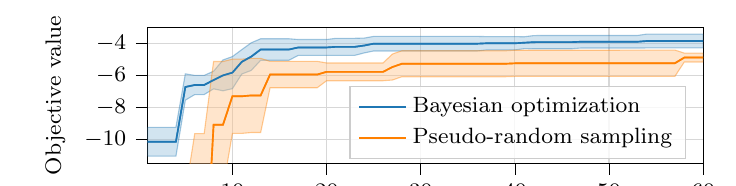
\begin{tikzpicture}[x=1in,y=1in]
  \useasboundingbox (-0.6, 0) rectangle (2.8, -0.65); %
    
  \definecolor{darkgrey176}{RGB}{176,176,176}
  \definecolor{lightgrey204}{RGB}{204,204,204}
  \definecolor{steelblue31119180}{RGB}{31,119,180}

  \begin{axis}[
  anchor=north west,
  width=3.4in,
  height=1.3in,
  legend cell align={left},
  legend style={
    fill opacity=0.8,
    draw opacity=1,
    text opacity=1,
    at={(0.97,0.03)},
    anchor=south east,
    font=\footnotesize,
    draw=lightgrey204
  },
  tick align=outside,
  tick pos=left,
  x grid style={darkgrey176!50},
  xlabel={Episodes},
  xmajorgrids,
  xmin=1, xmax=60,
  xtick style={color=black},
  y grid style={darkgrey176!50},
  ylabel={Objective value},
  ymajorgrids,
  xlabel shift=-1mm,
  ymin=-11.5, ymax=-3.0,
  ytick style={color=black},
  tick label style={font=\footnotesize}, %
  label style={font=\footnotesize}, %
  ]

  \addplot [semithick, steelblue31119180]
  table {%
  1 -10.1574191633144
  2 -10.1574191633144
  3 -10.1574191633144
  4 -10.1574191633144
  5 -6.72289483906331
  6 -6.59684858181106
  7 -6.59684858181106
  8 -6.28596903298211
  9 -5.99373655494911
  10 -5.82167779703389
  11 -5.1428110983115
  12 -4.81673457286373
  13 -4.37088875274734
  14 -4.37088875274734
  15 -4.37088875274734
  16 -4.37088875274734
  17 -4.24148141205882
  18 -4.24148141205882
  19 -4.24148141205882
  20 -4.24148141205882
  21 -4.20245990000189
  22 -4.20245990000189
  23 -4.20245990000189
  24 -4.11959725018268
  25 -4.00556881763445
  26 -4.00556881763445
  27 -4.00556881763445
  28 -4.00556881763445
  29 -4.00556881763445
  30 -4.00556881763445
  31 -4.00556881763445
  32 -4.00556881763445
  33 -4.00556881763445
  34 -4.00556881763445
  35 -4.00556881763445
  36 -4.00556881763445
  37 -3.97949251478588
  38 -3.97949251478588
  39 -3.97949251478588
  40 -3.97949251478588
  41 -3.94404729277079
  42 -3.91049026608397
  43 -3.90720589167441
  44 -3.90720589167441
  45 -3.90720589167441
  46 -3.90720589167441
  47 -3.88429011242476
  48 -3.88429011242476
  49 -3.88429011242476
  50 -3.88429011242476
  51 -3.88429011242476
  52 -3.88429011242476
  53 -3.88429011242476
  54 -3.83778249975218
  55 -3.83778249975218
  56 -3.83778249975218
  57 -3.83778249975218
  58 -3.83778249975218
  59 -3.83778249975218
  60 -3.83778249975218
  };
  \addlegendentry{Bayesian optimization}

  \path [draw=steelblue31119180!100, fill=steelblue31119180!50, opacity=0.4]
  (axis cs:1,-9.25192272947796)
  --(axis cs:1,-11.0629155971508)
  --(axis cs:2,-11.0629155971508)
  --(axis cs:3,-11.0629155971508)
  --(axis cs:4,-11.0629155971508)
  --(axis cs:5,-7.54939492206937)
  --(axis cs:6,-7.19721439515581)
  --(axis cs:7,-7.19721439515581)
  --(axis cs:8,-6.8386905924942)
  --(axis cs:9,-6.96114920237258)
  --(axis cs:10,-6.82854865024866)
  --(axis cs:11,-5.90839733741554)
  --(axis cs:12,-5.68382706642718)
  --(axis cs:13,-5.04568387720924)
  --(axis cs:14,-5.04568387720924)
  --(axis cs:15,-5.04568387720924)
  --(axis cs:16,-5.04568387720924)
  --(axis cs:17,-4.73792464284913)
  --(axis cs:18,-4.73792464284913)
  --(axis cs:19,-4.73792464284913)
  --(axis cs:20,-4.73792464284913)
  --(axis cs:21,-4.73733099029819)
  --(axis cs:22,-4.73733099029819)
  --(axis cs:23,-4.73733099029819)
  --(axis cs:24,-4.58459002120253)
  --(axis cs:25,-4.46280980134367)
  --(axis cs:26,-4.46280980134367)
  --(axis cs:27,-4.46280980134367)
  --(axis cs:28,-4.46280980134367)
  --(axis cs:29,-4.46280980134367)
  --(axis cs:30,-4.46280980134367)
  --(axis cs:31,-4.46280980134367)
  --(axis cs:32,-4.46280980134367)
  --(axis cs:33,-4.46280980134367)
  --(axis cs:34,-4.46280980134367)
  --(axis cs:35,-4.46280980134367)
  --(axis cs:36,-4.46280980134367)
  --(axis cs:37,-4.39831635351107)
  --(axis cs:38,-4.39831635351107)
  --(axis cs:39,-4.39831635351107)
  --(axis cs:40,-4.39831635351107)
  --(axis cs:41,-4.31605252044889)
  --(axis cs:42,-4.32412394230932)
  --(axis cs:43,-4.32527023808848)
  --(axis cs:44,-4.32527023808848)
  --(axis cs:45,-4.32527023808848)
  --(axis cs:46,-4.32527023808848)
  --(axis cs:47,-4.27735676012639)
  --(axis cs:48,-4.27735676012639)
  --(axis cs:49,-4.27735676012639)
  --(axis cs:50,-4.27735676012639)
  --(axis cs:51,-4.27735676012639)
  --(axis cs:52,-4.27735676012639)
  --(axis cs:53,-4.27735676012639)
  --(axis cs:54,-4.27143218019298)
  --(axis cs:55,-4.27143218019298)
  --(axis cs:56,-4.27143218019298)
  --(axis cs:57,-4.27143218019298)
  --(axis cs:58,-4.27143218019298)
  --(axis cs:59,-4.27143218019298)
  --(axis cs:60,-4.27143218019298)
  --(axis cs:60,-3.40413281931137)
  --(axis cs:60,-3.40413281931137)
  --(axis cs:59,-3.40413281931137)
  --(axis cs:58,-3.40413281931137)
  --(axis cs:57,-3.40413281931137)
  --(axis cs:56,-3.40413281931137)
  --(axis cs:55,-3.40413281931137)
  --(axis cs:54,-3.40413281931137)
  --(axis cs:53,-3.49122346472314)
  --(axis cs:52,-3.49122346472314)
  --(axis cs:51,-3.49122346472314)
  --(axis cs:50,-3.49122346472314)
  --(axis cs:49,-3.49122346472314)
  --(axis cs:48,-3.49122346472314)
  --(axis cs:47,-3.49122346472314)
  --(axis cs:46,-3.48914154526035)
  --(axis cs:45,-3.48914154526035)
  --(axis cs:44,-3.48914154526035)
  --(axis cs:43,-3.48914154526035)
  --(axis cs:42,-3.49685658985863)
  --(axis cs:41,-3.57204206509268)
  --(axis cs:40,-3.56066867606069)
  --(axis cs:39,-3.56066867606069)
  --(axis cs:38,-3.56066867606069)
  --(axis cs:37,-3.56066867606069)
  --(axis cs:36,-3.54832783392523)
  --(axis cs:35,-3.54832783392523)
  --(axis cs:34,-3.54832783392523)
  --(axis cs:33,-3.54832783392523)
  --(axis cs:32,-3.54832783392523)
  --(axis cs:31,-3.54832783392523)
  --(axis cs:30,-3.54832783392523)
  --(axis cs:29,-3.54832783392523)
  --(axis cs:28,-3.54832783392523)
  --(axis cs:27,-3.54832783392523)
  --(axis cs:26,-3.54832783392523)
  --(axis cs:25,-3.54832783392523)
  --(axis cs:24,-3.65460447916283)
  --(axis cs:23,-3.6675888097056)
  --(axis cs:22,-3.6675888097056)
  --(axis cs:21,-3.6675888097056)
  --(axis cs:20,-3.74503818126851)
  --(axis cs:19,-3.74503818126851)
  --(axis cs:18,-3.74503818126851)
  --(axis cs:17,-3.74503818126851)
  --(axis cs:16,-3.69609362828544)
  --(axis cs:15,-3.69609362828544)
  --(axis cs:14,-3.69609362828544)
  --(axis cs:13,-3.69609362828544)
  --(axis cs:12,-3.94964207930029)
  --(axis cs:11,-4.37722485920747)
  --(axis cs:10,-4.81480694381912)
  --(axis cs:9,-5.02632390752564)
  --(axis cs:8,-5.73324747347001)
  --(axis cs:7,-5.99648276846631)
  --(axis cs:6,-5.99648276846631)
  --(axis cs:5,-5.89639475605725)
  --(axis cs:4,-9.25192272947796)
  --(axis cs:3,-9.25192272947796)
  --(axis cs:2,-9.25192272947796)
  --(axis cs:1,-9.25192272947796)
  --cycle;

  \addplot [semithick, orange]
  table {%
  1 -24.8117548316848
  2 -24.8117548316848
  3 -24.8117548316848
  4 -24.8117548316848
  5 -23.9097738609303
  6 -20.0768245547915
  7 -20.0768245547915
  8 -9.09489985281767
  9 -9.09489985281767
  10 -7.30449400207115
  11 -7.30449400207115
  12 -7.25275367414012
  13 -7.25275367414012
  14 -5.94324016597094
  15 -5.94324016597094
  16 -5.94324016597094
  17 -5.94324016597094
  18 -5.94324016597094
  19 -5.94324016597094
  20 -5.77141780882547
  21 -5.77141780882547
  22 -5.77141780882547
  23 -5.77141780882547
  24 -5.77141780882547
  25 -5.77141780882547
  26 -5.77141780882547
  27 -5.46955325648097
  28 -5.26388748129056
  29 -5.26388748129056
  30 -5.26388748129056
  31 -5.26388748129056
  32 -5.26388748129056
  33 -5.26388748129056
  34 -5.26388748129056
  35 -5.26388748129056
  36 -5.26388748129056
  37 -5.26388748129056
  38 -5.26388748129056
  39 -5.26388748129056
  40 -5.23696661156889
  41 -5.23696661156889
  42 -5.23696661156889
  43 -5.23696661156889
  44 -5.23696661156889
  45 -5.23696661156889
  46 -5.23696661156889
  47 -5.23696661156889
  48 -5.23696661156889
  49 -5.23696661156889
  50 -5.23696661156889
  51 -5.23696661156889
  52 -5.22987952313497
  53 -5.22987952313497
  54 -5.22987952313497
  55 -5.22987952313497
  56 -5.22987952313497
  57 -5.22987952313497
  58 -4.8758610705042
  59 -4.8758610705042
  60 -4.8758610705042
  };
  \addlegendentry{Pseudo-random sampling}

  \path [draw=orange!100, fill=orange!50, opacity=0.4]
  (axis cs:1,-15.8254505980391)
  --(axis cs:1,-33.7980590653305)
  --(axis cs:2,-33.7980590653305)
  --(axis cs:3,-33.7980590653305)
  --(axis cs:4,-33.7980590653305)
  --(axis cs:5,-34.4583549633831)
  --(axis cs:6,-30.500835698174)
  --(axis cs:7,-30.500835698174)
  --(axis cs:8,-13.0650976691005)
  --(axis cs:9,-13.0650976691005)
  --(axis cs:10,-9.63305186269427)
  --(axis cs:11,-9.63305186269427)
  --(axis cs:12,-9.57854407058712)
  --(axis cs:13,-9.57854407058712)
  --(axis cs:14,-6.7726501658824)
  --(axis cs:15,-6.7726501658824)
  --(axis cs:16,-6.7726501658824)
  --(axis cs:17,-6.7726501658824)
  --(axis cs:18,-6.7726501658824)
  --(axis cs:19,-6.7726501658824)
  --(axis cs:20,-6.32853325564196)
  --(axis cs:21,-6.32853325564196)
  --(axis cs:22,-6.32853325564196)
  --(axis cs:23,-6.32853325564196)
  --(axis cs:24,-6.32853325564196)
  --(axis cs:25,-6.32853325564196)
  --(axis cs:26,-6.32853325564196)
  --(axis cs:27,-6.28418882407104)
  --(axis cs:28,-6.07760333508252)
  --(axis cs:29,-6.07760333508252)
  --(axis cs:30,-6.07760333508252)
  --(axis cs:31,-6.07760333508252)
  --(axis cs:32,-6.07760333508252)
  --(axis cs:33,-6.07760333508252)
  --(axis cs:34,-6.07760333508252)
  --(axis cs:35,-6.07760333508252)
  --(axis cs:36,-6.07760333508252)
  --(axis cs:37,-6.07760333508252)
  --(axis cs:38,-6.07760333508252)
  --(axis cs:39,-6.07760333508252)
  --(axis cs:40,-6.05896797065684)
  --(axis cs:41,-6.05896797065684)
  --(axis cs:42,-6.05896797065684)
  --(axis cs:43,-6.05896797065684)
  --(axis cs:44,-6.05896797065684)
  --(axis cs:45,-6.05896797065684)
  --(axis cs:46,-6.05896797065684)
  --(axis cs:47,-6.05896797065684)
  --(axis cs:48,-6.05896797065684)
  --(axis cs:49,-6.05896797065684)
  --(axis cs:50,-6.05896797065684)
  --(axis cs:51,-6.05896797065684)
  --(axis cs:52,-6.05436508485352)
  --(axis cs:53,-6.05436508485352)
  --(axis cs:54,-6.05436508485352)
  --(axis cs:55,-6.05436508485352)
  --(axis cs:56,-6.05436508485352)
  --(axis cs:57,-6.05436508485352)
  --(axis cs:58,-5.15323923666181)
  --(axis cs:59,-5.15323923666181)
  --(axis cs:60,-5.15323923666181)
  --(axis cs:60,-4.59848290434659)
  --(axis cs:60,-4.59848290434659)
  --(axis cs:59,-4.59848290434659)
  --(axis cs:58,-4.59848290434659)
  --(axis cs:57,-4.40539396141641)
  --(axis cs:56,-4.40539396141641)
  --(axis cs:55,-4.40539396141641)
  --(axis cs:54,-4.40539396141641)
  --(axis cs:53,-4.40539396141641)
  --(axis cs:52,-4.40539396141641)
  --(axis cs:51,-4.41496525248093)
  --(axis cs:50,-4.41496525248093)
  --(axis cs:49,-4.41496525248093)
  --(axis cs:48,-4.41496525248093)
  --(axis cs:47,-4.41496525248093)
  --(axis cs:46,-4.41496525248093)
  --(axis cs:45,-4.41496525248093)
  --(axis cs:44,-4.41496525248093)
  --(axis cs:43,-4.41496525248093)
  --(axis cs:42,-4.41496525248093)
  --(axis cs:41,-4.41496525248093)
  --(axis cs:40,-4.41496525248093)
  --(axis cs:39,-4.45017162749861)
  --(axis cs:38,-4.45017162749861)
  --(axis cs:37,-4.45017162749861)
  --(axis cs:36,-4.45017162749861)
  --(axis cs:35,-4.45017162749861)
  --(axis cs:34,-4.45017162749861)
  --(axis cs:33,-4.45017162749861)
  --(axis cs:32,-4.45017162749861)
  --(axis cs:31,-4.45017162749861)
  --(axis cs:30,-4.45017162749861)
  --(axis cs:29,-4.45017162749861)
  --(axis cs:28,-4.45017162749861)
  --(axis cs:27,-4.65491768889089)
  --(axis cs:26,-5.21430236200899)
  --(axis cs:25,-5.21430236200899)
  --(axis cs:24,-5.21430236200899)
  --(axis cs:23,-5.21430236200899)
  --(axis cs:22,-5.21430236200899)
  --(axis cs:21,-5.21430236200899)
  --(axis cs:20,-5.21430236200899)
  --(axis cs:19,-5.11383016605948)
  --(axis cs:18,-5.11383016605948)
  --(axis cs:17,-5.11383016605948)
  --(axis cs:16,-5.11383016605948)
  --(axis cs:15,-5.11383016605948)
  --(axis cs:14,-5.11383016605948)
  --(axis cs:13,-4.92696327769312)
  --(axis cs:12,-4.92696327769312)
  --(axis cs:11,-4.97593614144803)
  --(axis cs:10,-4.97593614144803)
  --(axis cs:9,-5.12470203653484)
  --(axis cs:8,-5.12470203653484)
  --(axis cs:7,-9.65281341140902)
  --(axis cs:6,-9.65281341140902)
  --(axis cs:5,-13.3611927584774)
  --(axis cs:4,-15.8254505980391)
  --(axis cs:3,-15.8254505980391)
  --(axis cs:2,-15.8254505980391)
  --(axis cs:1,-15.8254505980391)
  --cycle;


  \addplot [semithick, steelblue31119180]
  table {%
  1 -10.1574191633144
  2 -10.1574191633144
  3 -10.1574191633144
  4 -10.1574191633144
  5 -6.72289483906331
  6 -6.59684858181106
  7 -6.59684858181106
  8 -6.28596903298211
  9 -5.99373655494911
  10 -5.82167779703389
  11 -5.1428110983115
  12 -4.81673457286373
  13 -4.37088875274734
  14 -4.37088875274734
  15 -4.37088875274734
  16 -4.37088875274734
  17 -4.24148141205882
  18 -4.24148141205882
  19 -4.24148141205882
  20 -4.24148141205882
  21 -4.20245990000189
  22 -4.20245990000189
  23 -4.20245990000189
  24 -4.11959725018268
  25 -4.00556881763445
  26 -4.00556881763445
  27 -4.00556881763445
  28 -4.00556881763445
  29 -4.00556881763445
  30 -4.00556881763445
  31 -4.00556881763445
  32 -4.00556881763445
  33 -4.00556881763445
  34 -4.00556881763445
  35 -4.00556881763445
  36 -4.00556881763445
  37 -3.97949251478588
  38 -3.97949251478588
  39 -3.97949251478588
  40 -3.97949251478588
  41 -3.94404729277079
  42 -3.91049026608397
  43 -3.90720589167441
  44 -3.90720589167441
  45 -3.90720589167441
  46 -3.90720589167441
  47 -3.88429011242476
  48 -3.88429011242476
  49 -3.88429011242476
  50 -3.88429011242476
  51 -3.88429011242476
  52 -3.88429011242476
  53 -3.88429011242476
  54 -3.83778249975218
  55 -3.83778249975218
  56 -3.83778249975218
  57 -3.83778249975218
  58 -3.83778249975218
  59 -3.83778249975218
  60 -3.83778249975218
  };
  


  \addplot [semithick, orange]
  table {%
  1 -24.8117548316848
  2 -24.8117548316848
  3 -24.8117548316848
  4 -24.8117548316848
  5 -23.9097738609303
  6 -20.0768245547915
  7 -20.0768245547915
  8 -9.09489985281767
  9 -9.09489985281767
  10 -7.30449400207115
  11 -7.30449400207115
  12 -7.25275367414012
  13 -7.25275367414012
  14 -5.94324016597094
  15 -5.94324016597094
  16 -5.94324016597094
  17 -5.94324016597094
  18 -5.94324016597094
  19 -5.94324016597094
  20 -5.77141780882547
  21 -5.77141780882547
  22 -5.77141780882547
  23 -5.77141780882547
  24 -5.77141780882547
  25 -5.77141780882547
  26 -5.77141780882547
  27 -5.46955325648097
  28 -5.26388748129056
  29 -5.26388748129056
  30 -5.26388748129056
  31 -5.26388748129056
  32 -5.26388748129056
  33 -5.26388748129056
  34 -5.26388748129056
  35 -5.26388748129056
  36 -5.26388748129056
  37 -5.26388748129056
  38 -5.26388748129056
  39 -5.26388748129056
  40 -5.23696661156889
  41 -5.23696661156889
  42 -5.23696661156889
  43 -5.23696661156889
  44 -5.23696661156889
  45 -5.23696661156889
  46 -5.23696661156889
  47 -5.23696661156889
  48 -5.23696661156889
  49 -5.23696661156889
  50 -5.23696661156889
  51 -5.23696661156889
  52 -5.22987952313497
  53 -5.22987952313497
  54 -5.22987952313497
  55 -5.22987952313497
  56 -5.22987952313497
  57 -5.22987952313497
  58 -4.8758610705042
  59 -4.8758610705042
  60 -4.8758610705042
  };
  
  
  \addplot [very thick, black, dash pattern=on 11.1pt off 4.8pt]
  table {%
  0 0
  59 0
  };
  \end{axis}

  \end{tikzpicture}

\clearpage
 \section{Introduction}
% \lipsum[2-3]
%%%%%%%%%%%%%%%%%%%%%%%%%%%%%%%%%%%%%%%%%%%%%%%%%%%%%%%%%%%%%%%%%%%%%%%%%%%%%%%%%%%
%Ultrasound in general
% Medical ultrasound, thanks to its non-invasiveness, portability, real-time performance, and wide affordability, is frequently used in daily clinical practice for screening and intra-operative guidance. 
% Despite these advantages, traditional free-hand ultrasound examinations also suffer from inter- and intra-operator variances.
% The quality of ultrasound images is affected by various acquisition parameters, including contact forces, acquisition angles, probe positioning, etc~\cite{tan2023autonomous,huang2018robotic}. These factors make ultrasound imaging highly operator-dependent, which, in turn, reduces the reproducibility of the results~\cite{tan2022flexible}. To tackle such a dilemma, the robotic ultrasound system (RUSS) demonstrates the potential to offer a promising solution~\cite{jiang2023robotic, akbari2021robot,bi2024machine}.
Medical ultrasound, valued for its non-invasiveness, portability, real-time performance, and affordability, is widely used in clinical practice for screening and intra-operative guidance. However, traditional free-hand ultrasound suffers from inter- and intra-operator variances. Image quality depends on acquisition parameters like contact forces, angles, and probe positioning~\cite{tan2023autonomous,huang2018robotic}, making it highly operator-dependent and reducing result reproducibility~\cite{tan2022flexible}. To tackle such a dilemma, robotic ultrasound systems (RUSS) offer a promising solution to address these challenges~\cite{jiang2023robotic, akbari2021robot,bi2024machine}.

\par
Owing to the fast development in the field of robotics, robots have shown their superiority over humans in terms of stability and precision.
Working together with human experts as colleagues, the interactive RUSS can largely release the burden of cumbersome acquisition from sonographers and greatly enhance the reproducibility of the imaging process~\cite{li2021overview,von2021medical,huang2023review}.
% RUSSs have been introduced to perform vascular ultrasound screening autonomously~\cite{jiang2021autonomous,huangQ2024robot}. 
% However, the distribution of human vessels is complicated and full of branches. 
% Therefore, it is common to have multiple vessels or bifurcation in ultrasound images. In such cases, it is important to provide explicit human guidance to the system so that the robot can online adjust its movement to better visualize the vessel of interest.
% Besides, such guidance can also be utilized by the segmentation network as a region proposal to improve the vessel segmentation results, especially for the limb vessels, which are small in size ($2.70\pm0.15$ mm)~\cite{wahood2022radial}, making them hard to be extracted precisely and robustly from B-mode images.
RUSSs are used for autonomous vascular ultrasound screening~\cite{jiang2021autonomous,huangQ2024robot}, but the complexity of vessel distributions and branches often results in multiple vessels or bifurcations in images. Explicit human guidance is essential for online robotic adjustments to better visualize target vessels. This guidance also aids segmentation networks as region proposals, improving vessel segmentation, particularly for small limb vessels ($2.70\pm0.15$ mm)~\cite{wahood2022radial}, which are challenging to extract accurately from B-mode images.

\par
In order to tackle the aforementioned challenges, this work proposes a gaze-guided RUSS. Gaze tracker, as an intuitive and efficient tool for human-machine interaction, has been widely applied to various medical robotic systems~\cite{noonan2008gaze,tong2015retrofit,guo2019novel}. This study presents the first exploration of integrating gaze tracking into RUSSs, allowing the system to incorporate real-time human supervision to improve the intelligence and robustness of the RUSS during complex scanning tasks. 
Especially in intra-operative ultrasound imaging, the hands of surgeons are often occupied with essential surgical tools such as needles or catheters, making manual maneuvering of the ultrasound probe challenging. Implementing a gaze tracker as a part of the RUSS helps the operators control the ultrasound scanning without disrupting the surgical workflow.
On one hand, the eye tracking information can indicate the vessel of interest during the scanning. On the other hand, the gaze of the operator can also be applied as network attention to assist the vessel segmentation, particularly for challenging ones with limited size. Based on the segmentation results, the robot is controlled to adapt its maneuvers so that the vessel of interest is kept in the middle of the ultrasound image. To further improve the ultrasound image quality during scanning, a confidence-driven control for linear ultrasound probes is proposed. The main contributions of this article are listed as follows:\footnote{\final{Codes: \url{https://github.com/yuan-12138/Gaze_RUSS}}}\footnote{\final{Video: \url{https://www.youtube.com/watch?v=Zul2-fqy0FE}}}
\begin{itemize}
  \item \revision{A gaze-guided segmentation network is proposed, which effectively integrates attention heatmaps derived from gaze patterns into segmentation. This improves segmentation performance by enabling the system to focus on the relevant regions in ultrasound images and providing the ability to segment vessels based on the operator's gaze.}
  \item  \revision{A human intention estimation module is introduced to predict the operator's intention during scanning by combining gaze patterns with segmentation result history. This module stabilizes noisy gaze signals, providing consistent and reliable guidance to the segmentation network.}
  \item \revision{A gaze-guided RUSS is developed and validated on a realistic arm phantom, showcasing its ability to perform complex scans. The system dynamically switched focus between vessels based on the operator's eye tracking, while the confidence-driven control method continuously adjusted probe orientation to optimize image quality.}
\end{itemize}

\par
To emphasize realism, we highlight that the proposed gaze-guided RUSS does not rely on highly stable gaze input from clinicians. The system can still operate with the intermittent absence of gaze input by using a zero-value map as the gaze attention heatmap (see Sec.~\ref{sec_gaze_guided_seg}). When necessary it can seamlessly integrate the operator's input, such as when adjusting the scanning focus for complex scenarios like bifurcations.

\begin{figure*}[ht!]
\centering
\includegraphics[width=0.8\textwidth]{images/overview.png}
\caption{
% Overview of the Proposed Gaze-Guided Interactive RUSS: The human gaze signal, captured by a gaze tracker, is combined with segmentation results history in a human intention estimation module to infer the operator's actual intention, particularly when multiple vessels are visible in the ultrasound image. The generated attention heatmap is then fed into the gaze-guided segmentation network, guiding it to produce accurate segmentation masks for the vessel of interest. The segmentation results are integrated into the robotic control loop, ensuring that the target vessel remains centered in the ultrasound image. To improve contact with the curved surface and enhance ultrasound image quality, a confidence-based orientation correction is applied. The red boxes in the ultrasound images highlight shadowed areas caused by improper probe contact.
Overview of the Proposed Gaze-Guided Interactive RUSS: The human gaze signal, captured by a gaze tracker, is combined with segmentation history in an intention estimation module to infer the operator's preference, especially when multiple vessels are visible. The resulting attention heatmap guides the gaze-guided segmentation network to produce accurate vessel segmentation masks. These results are integrated into the robotic control loop to keep the target vessel centered in the ultrasound image. A confidence-based orientation correction optimizes probe contact with curved surfaces, improving image quality. Red boxes in ultrasound images highlight shadowed areas caused by improper probe contact.
}
\label{Fig_overview}
\end{figure*}


%%%%%%%%%%%%%%%%%%%%%%%%%%%%%%
\section{Related Work}
% RUSS
\subsection{Robotic Ultrasound Systems}
Ultrasound image quality depends heavily on acquisition parameters such as force, orientation, and surface contact. To address this, Pierrot~\emph{et al.}~\cite{pierrot1999hippocrate} implemented a force control schema in a teleoperative RUSS to maintain constant scanning force. Jiang~\emph{et al.}~\cite{jiang2020automatic} introduced an orientation optimization algorithm based on contact force for better visualization.
To ensure that the ultrasound probe is in good contact with the surface, Chatelain~\emph{et al.}~\cite{chatelain2017confidence} integrated ultrasound confidence map~\cite{karamalis2012ultrasound} into the control loop and presented confidence-driven control. However, the proposed control algorithm was designed for convex probe. In the sight of such limitation, Jiang~\emph{et al.}~\cite{jiang2022precise} proposed an orientation correction method based on the confidence map for the linear probes. The experimental results clearly demonstrated its effectiveness, but the theoretical justification is missing.

\par
Recent advancements in RUSS for vascular applications have gained significant attention. Jiang~\emph{et al.}~\cite{jiang2021autonomous} proposed an autonomous scanning framework for peripheral vascular diseases using real-time vessel segmentation. Bi~\emph{et al.}~\cite{bi2022vesnet} applied reinforcement learning to autonomously navigate the probe to the longitudinal view of the carotid artery. Huang~\emph{et al.}~\cite{huangQ2024robot} developed a system to autonomously perform carotid scans by imitating clinical protocols, while Goel~\emph{et al.}~\cite{goel2022autonomous} introduced a Bayesian Optimization-based path planning framework for femoral artery screening.

\par
\revision{
Most existing RUSSs for vascular scanning do not address the challenge of handling multiple vessels and often require additional tools to capture the doctor's intention for automatic maneuvering. Guidance can be implemented teleoperatively, with an expert operating remotely while the robot on-site follows~\cite{fu2022robot}, or through virtual reality, providing virtual guidance to the human operator~\cite{black2024human}. Another approach involves pre-planned scanning paths, where the robot provides virtual fixtures to enable reproducible ultrasound scanning for follow-up validations~\cite{huang2024robot}. However, among these strategies, gaze signal—an intuitive and hands-free interaction method—remains unexplored. This approach is particularly advantageous in intra-operative scenarios, as it allows surgeons to perform tasks without altering workflow.}

% Gaze-guided Medical Robotic Systems
\subsection{Gaze-guided Medical Robotic Systems}
Initial attempts to integrate gaze information into medical robotic systems have been made in various scenarios, especially for laparoscopic surgeries. 
Noonan~\emph{et al.}~\cite{noonan2010gaze} used eye tracking to control an articulated robotic laparoscope for stable, hands-free visualization. Fujii~\emph{et al.}~\cite{fujii2018gaze} enhanced the gaze-guided laparoscope maneuverability by using a robotic arm instead of a rigid fixture. Clancy~\emph{et al.}~\cite{clancy2011gaze} combined gaze tracking with a liquid lens in the da Vinci system for automatic focus adjustment during minimally invasive surgeries. Gaze tracking has also been applied to constrain laparoscopic surgical tools for tissue safety~\cite{mylonas2012gaze} and to improve collaboration in multi-robot surgeries by visualizing fixation points~\cite{kwok2012collaborative}. Li~\emph{et al.}~\cite{li2018free} further optimized gaze tracking accuracy by compensating for head movements.
Beyond laparoscopic applications, Guo~\emph{et al.}~\cite{guo2019novel} utilized gaze to control needle insertion in CT-guided interventions, while Kogkas~\emph{et al.}~\cite{kogkas2019free} introduced a gaze-guided robotic scrub nurse to deliver surgical tools. To the best of our knowledge, initial attempt to integrate the gaze tracker into RUSS has not yet occurred.

% Gaze-guided Network
\subsection{Gaze-guided Medical Image Analysis}\label{sec_gaze_med_IA}
Unlike optical images, medical images are often challenging to interpret, requiring solid biological knowledge for accurate diagnostics. To enhance the robustness of medical image analysis networks, human experts' gaze signals are frequently integrated as guidance. Cai~\emph{et al.}~\cite{cai2020spatio} proposed Temporal SonoEyeNet, which predicts sonographers' visual attention and ultrasound standard planes, demonstrating that understanding visual attention complements standard plane detection. Similarly, Wang~\emph{et al.}~\cite{wang2022follow} used class activation maps~\cite{zhou2016learning} to align network attention with human gaze.
In another application, Men~\emph{et al.}~\cite{men2023gaze} leveraged gaze tracking to improve probe movement prediction for obstetric standard plane navigation, while Alsharid~\emph{et al.}~\cite{alsharid2022gaze} showed its benefits in ultrasound video captioning. Most of these works aim to align networks with human attention to enhance reasoning. Beyond implicit guidance, gaze signals also serve as an intuitive tool for human-machine interaction. For instance, Khosravan~\emph{et al.}~\cite{khosravan2019collaborative} developed a collaborative lesion segmentation system that analyzes and filters doctors' gaze data to improve segmentation and reduce false positives.

%%%%%%%%%%%%%%%%%%%%%%%%%%%%%%%%%%%%%%%%%%%%%%%%%%%%%%%%%%%%%%%%%%%%%%%%%%%%%%%%%%%%%%%%%%%%%%%%%%%%%%%%%%%%%%%%%%%%%%%%%%%%%%

\section{Methods}
As shown in Fig.~\ref{Fig_overview}, the proposed gaze-guided RUSS consists of two main components: image processing and robotic control. The human operator’s gaze signal is fed into an attention-estimation module, which uses sequential segmentation results and gaze tracking history to predict the operator's actual attention. It is important to distinguish between the gaze heatmap, directly captured by the eye tracker, and the attention heatmap, which reflects the operator's true focus.
Sonographers often glance at other areas of the ultrasound image to maintain contextual awareness of surrounding anatomical structures, rather than focusing solely on the vessel of interest. Differentiating these incidental glances from an intentional focus shift is critical to ensure the RUSS follows the correct vessel and avoids unnecessary target switches.
The estimated attention heatmap guides the gaze-guided segmentation network to extract the vessel of interest from the ultrasound image. The resulting segmentation directs the robot to center the vessel in the ultrasound image. To maintain good probe contact with the scanning surface, a confidence-driven orientation correction is implemented, adjusting the probe’s rotation around its y-axis based on the ultrasound confidence map to enhance image quality. During acquisition, impedance control~\cite{jiang2021autonomous} is employed to maintain consistent contact force.

\begin{figure*}[ht!]
\centering
\includegraphics[width=0.8\textwidth]{images/Gaze_UNet_trans.png}
\caption{(a) The overall design of the proposed gaze-guided segmentation network. (b) The structure of the transformer attention block. (c) The structure of the residual block.
}
\label{Fig_segmentation}
\end{figure*}

\subsection{Gaze-Guided Segmentation Network}\label{sec_gaze_guided_seg}
\revision{During the training of the proposed segmentation network, pseudo attention maps are generated from the label maps of B-mode ultrasound images and paired with ultrasound images to simulate human attention on vessels. This approach addresses the instability and noise in real gaze signals, which could mislead the network, and the difficulty of directly obtaining human attention heatmaps. By incorporating randomness into their generation, these pseudo attention maps create a more diverse and extensive dataset, reducing bias and improving the network's robustness and generalization.}
The pseudo attention heatmaps are generated based on the ground truth label maps. The centroid point of the heatmap ($X_m,Y_m$) is determined by the center point of the vessel label ($X_l,Y_l$).
\begin{align}
    (X_m, Y_m) &\sim \mathcal{N}\left( (X_l, Y_l), \Sigma_c \right) \\
    (x_m, y_m) &\sim \mathcal{N}\left( (X_m, Y_m), \Sigma_m \right)
\end{align}
where $\Sigma_c$ represents the covariance matrix of the Gaussian distribution. Based on the sampled centroid point of heatmap ($X_m,Y_m$), $N$ points ($x_m,y_m$) are selected and set to one.
The image that contains all the sampled points ($x_m,y_m$) is convolved by a $30\times30$ kernel with all weights setting to $1$. After the convolution, the resulting image is normalised to $[0,1]$. In this manner, a diffused heatmap $H$ is generated, simulating the density of the eye tracking points. Here $\Sigma_c\in R^{2\times2}$ and $\Sigma_m\in R^{2\times2}$ are diagonal matrices, with their diagonal values setting to 15 and 25, respectively.

\par
\revision{As depicted in Fig.~\ref{Fig_segmentation} (a), the segmentation network follows a U-shaped design. To enhance its performance, we incorporate attention heatmaps generated by the Human Intention Estimation Module based on human eye gaze signals. These maps represent the stabilized focus of the operator and are used to dynamically guide the network to prioritize the vessel of interest.}
\revision{A transformer attention block~\cite{vaswani2017attention} is incorporated to combine external attention signals from heatmaps with features extracted from ultrasound images. This adaptation enables the network to dynamically align its focus with the operator's intentions. As depicted in Fig.~\ref{Fig_segmentation} (b), the transformer attention block uses attention heatmaps as guidance to emphasize regions of interest. Inspired by~\cite{gao2021utnet}, subsampling is applied within the transformer block to reduce computational complexity. The transformed features are then concatenated with those from the ultrasound image encoder, facilitating the decoder's ability to generate precise segmentation masks.}

\par
If an ultrasound image contains multiple vessels, they are individually labeled and treated as distinct training samples to generate pseudo attention heatmaps. To reduce reliance on explicit guidance, $n\%$ of the generated attention maps are replaced with uniform maps where all weights are set to zero. This means that for $n\%$ of the training samples, no attention is provided, prompting the network to segment all vessels in the image independently. For this study, $n$ is set to $10\%$. This approach enhances the network’s adaptability, allowing gaze tracking to act as a performance booster rather than a critical component of the segmentation framework. During inference, pseudo attention heatmaps are replaced by the output of the attention estimation module (see Sec.~\ref{sec_estimation_m}).

\begin{figure}[ht!]
\centering
\includegraphics[width=0.4\textwidth]{images/Estimation_Module.png}
\caption{The design of the human intention estimation module.
}
\label{Fig_estimation_module}
\end{figure}


%%%%%%%%%%%%%%%%%%%%%%
\subsection{\revision{Stabilized Attention Heatmap Generation}}\label{sec_estimation_m}
Gaze heatmap is different from the human intention heatmap.
Although the attention of the operator remains focused on the target vessel, it is unrealistic for them to keep steering at it throughout the whole scanning process.
Instead, the sonographers tend to take glances at the surrounding anatomical structures to gain an overall contextual awareness. Therefore, without additional processing, the raw gaze heatmaps are not suitable to be directly used as attentions in the proposed segmentation network. In essence, the desired heatmap of the segmentation network should reveal the preference of the human operator among multiple vessels in the ultrasound image. 
\revision{To achieve this, the Human Intention Estimation Module analyzes sequential gaze patterns and segmentation label maps from previous timesteps, as shown in Fig.~\ref{Fig_estimation_module}. By combining these inputs, the module addresses the limitations of relying on gaze or segmentation history alone. For instance, if the segmentation history consistently focuses on a single vessel and the gaze heatmap briefly deviates, it is likely a temporal distraction. Conversely, stable deviation in the gaze heatmap suggests an intentional attention switch. This integration allows the network to reliably distinguish between temporal distractions and intentional changes in focus, ensuring robust guidance for segmentation.}

% network structure
\par
\revision{As shown in Fig.~\ref{Fig_estimation_module}, in our implementation, T=64 (approximately 2.13 seconds) was chosen empirically. This value aligns well with the average human fixation duration ($290\pm155$ ms)~\cite{henderson2015neural} and avoids the time delay associated with higher T values.}
Two 3D convolutional encoders are employed to extract features from the gaze signals and segmentation results, respectively. At each scale, the extracted 3D feature maps are transformed into 2D feature maps through $1\times1\times1$ 3D convolution. The transformed 2D features are then concatenated with upsampled features in decoder to generate the final attention heatmap for the segmentation network.

% training strategy
\par
For training, different gaze patterns are recorded from human operators serving as training data. During training, the well-trained weights of the segmentation network is frozen and the output attention map from the attention estimation module is fed into the segmentation network (see Fig.~\ref{Fig_segmentation}) to perform segmentation task. 
\revision{The resulting DICE loss between the predicted segmentation map and the ground truth label was backpropagated to update the weights of the attention estimation module. By utilizing the fixed segmentation network, the DICE loss guided the attention estimation module to output refined attention maps that align with the segmentation task, effectively training the module to infer human attention.}

\begin{figure}[ht!]
\centering
\includegraphics[width=0.453\textwidth]{images/confidence_control_lin.png}
\caption{The illustration of confidence-driven probe orientation correction for linear ultrasound probe. The red boxes in the images indicate the shadow areas caused by improper contact. $\{I\}$ represents the ultrasound imaging coordinate system, while $\{P\}$ is the probe coordinate system.
}
\label{Fig_conf_control}
\end{figure}

\subsection{Confidence-based Orientation Correction for Linear Probe}
The ultrasound probe's coordinate system is shown in Fig.~\ref{Fig_overview}. Translational movement along the z-axis is controlled using impedance control to ensure proper contact force with the scanning surface~\cite{jiang2021autonomous}. The y-axis represents forward motion during vessel scanning, while x-axis translation is guided by segmentation results to center the target vessel in the ultrasound image. In order to optimize the ultrasound image quality, a confidence-based orientation correction method for linear ultrasound probe is proposed.

\par
The confidence map~\cite{karamalis2012ultrasound} is widely used for assessing ultrasound image quality, assigning per-pixel confidence values based on a simplified sound propagation model. While the original confidence map relies on a computationally intensive random walk algorithm, the scan-line-based confidence map~\cite{chatelain2016quality} offers significantly improved efficiency.
To ensure real-time performance in the proposed confidence-driven control for the linear ultrasound probe, the scan-line-based confidence map is utilized. Let $I(x,y)$ denote the intensity value of a ultrasound image at position $(x,y)$ in the image coordination system. The scan-line-based confidence map is then given by:
\begin{equation}
    % C(X,Y)=1-\frac{\int_{0}^{Y}f(I(X,y))dy}{\int_{0}^{Y_{max}}f(I(X,y))dy}
    C(X,Y)=1-\left(\int_{0}^{{Y}_{max}}f(I(X,y))dy\right)^{-1}\int_{0}^{Y}f(I(X,y))dy
\end{equation}
where $f(*)$ is a non-linear mapping function between the radiofrequency signal intensity and the gray scale image intensity $I$. Here, $f(x) = x^{2}$ is used.

\par
As shown in Fig.~\ref{Fig_conf_control}, dark regions in the confidence maps (highlighted by red rectangles) indicate improper contact between the ultrasound probe and the skin surface. To enhance image quality, a correction angle ($\theta_c$) is calculated to rotate the probe around its y-axis, improving the confidence level in the central region of the ultrasound image. The confidence-weighted centerline is determined as follows:
\begin{equation}
    x_c = \frac{1}{C_\Omega}\iint_{(x,y)\in\Omega}xC(x,y)ydydx
\end{equation}
where $C_{\Omega} = \iint_{(x,y)\in\Omega}C(x,y)ydydx$.
% \begin{equation}
%     C_{\Omega} = \iint_{(x,y)\in\Omega}C(x,y)ydydx
% \end{equation}
\par
The position of the confidence-weighted centerline can be viewed as the tangency point between the linear transducer and the curved surface. Then as shown in Fig.~\ref{Fig_conf_control}, the distance ($d_c$) between the confidence-weighted centerline and the image centerline is computed.
\begin{equation}\label{eq_d_c}
    d_c = x_c-X_{c}
\end{equation}
where $X_c$ is the position of the image centerline. Then, the correction angle $\theta_c$ can be computed using Eq~(\ref{eq_conf_correction}):
\begin{equation}\label{eq_conf_correction}
    \theta_c = arctan(\frac{d_c}{R})
\end{equation}
where $R$ is the radius of curvature in the ideal case, this would allow for a one-time adjustment. However, due to the varying curvature of the human body, accurately estimating this parameter online for human tissue is challenging, particularly considering the pressure-induced deformation. To address this, angular correction was performed using visual servoing mode. The parameter $d_c$ ensures final convergence, aligning the confidence-based centerline with the centerline of the ultrasound imaging plane of the linear probe. A small $R$ may cause fluctuations in movement. To balance motion smoothness with angular correction efficiency, $R$ was empirically set to $10~cm$ based on experimental results.

\begin{table*}[ht!]
\caption{\revision{Segmentation results (Dice Score) of different segmentation network architectures and the meta data of each volunteer.}}\label{tab:segmentation}\centering

  % \begin{tabular}{lc|c|c|c|c}
  \renewcommand{\arraystretch}{0.6}
  \resizebox{0.8\textwidth}{!}{
  \begin{tabular}{l l c| c| c| c| c}
    \toprule
    Method & Artery &$V_1$ & $V_2$ & $V_3$ & $V_4$ & $V_5$\\
    % \cmidrule{2-6}
    
    \midrule
    \multirow{2}{*}{UNet~\cite{ronneberger2015u}} & Radial & $0.456\pm 0.400$ & $0.562\pm 0.294$ & $0.084\pm 0.158$ & $0.401\pm 0.301$ & $0.292\pm 0.373$\\
    & Interosseous & $0.359\pm 0.276$ & $0.470\pm 0.297$ & $0.1821\pm 0.256$ & $0.467\pm 0.322$ & $0.389\pm 0.323$\\
    \cmidrule{2-7}
    \multirow{2}{*}{Att-UNet~\cite{schlemper2019attention}} & Radial & $0.486\pm 0.331$ & $0.611\pm 0.283$ & $0.254\pm 0.298$ & $0.708\pm 0.181$ & $0.385\pm 0.397$\\
    & Interosseous & $0.436\pm 0.283$ & $0.553\pm 0.224$ & $0.515\pm 0.377$ & $0.481\pm 0.340$ & $0.498\pm 0.278$\\
    \cmidrule{2-7}
    \multirow{2}{*}{UTNet~\cite{gao2021utnet}} & Radial & $0.671\pm 0.255$ & $0.710\pm 0.191$ & $0.275\pm 0.249$ & $0.748\pm 0.080$ & $0.263\pm 0.329$\\
    & Interosseous & $0.338\pm 0.207$ & $0.345\pm 0.314$ & $0.485\pm 0.288$ & $0.367\pm 0.250$ & $0.409\pm 0.302$\\
    \cmidrule{2-7}
    \multirow{2}{*}{UNet++~\cite{zhou2019unet++}} & Radial & $0.346\pm 0.332$ & $0.707\pm 0.221$ & $0.215\pm 0.223$ & $0.739\pm 0.090$ & $0.495\pm 0.259$\\
    & Interosseous & $0.442\pm 0.251$ & $0.421\pm 0.252$ & $0.581\pm 0.316$ & $0.242\pm 0.239$ & $0.549\pm 0.261$\\
    % \cmidrule{2-6}
    \midrule
    % Ours + Pseudo  & Radial & $0.714\pm 0.150$ & $0.717\pm 0.266$ & $0.308\pm 0.316$ & $0.799\pm 0.080$ & $0.618\pm 0.280$\\
    % Att. Heatmap & Interosseous & $0.553\pm 0.201$ & $0.707\pm 0.156$ & $0.758\pm 0.137$ & $0.683\pm 0.195$ & $0.575\pm 0.295$\\
    % \cmidrule{2-7}
    Ours + Pseudo  & Radial & $\mathbf{0.794\pm 0.130}$ & $\mathbf{0.740\pm 0.199}$ & $\mathbf{0.389\pm 0.346}$ & $\mathbf{0.880\pm 0.053}$ & $0.709\pm 0.263$\\
    Att. Heatmap & Interosseous & $0.603\pm 0.223$ & $0.672\pm 0.185$ & $0.741\pm 0.241$ & $\mathbf{0.755\pm 0.165}$ & $\mathbf{0.746\pm 0.166}$\\
    \cmidrule{2-7}
    Ours + Raw & Radial & $0.500\pm 0.423$ & $0.585\pm 0.351$ & $0.259\pm 0.309$ & $0.602\pm 0.384$ & $0.404\pm 0.336$\\
    Gaze Heatmap & Interosseous & $0.212\pm 0.235$ & $0.659\pm 0.167$ & $0.563\pm 0.290$ & $0.558\pm 0.327$ & $0.428\pm 0.329$\\
    \cmidrule{2-7}
    Ours + Est. & Radial & $0.736\pm 0.295$ & $0.721\pm 0.255$ & $0.335\pm 0.322$ & $0.822\pm 0.090$ & $\mathbf{0.737\pm 0.145}$\\
    Att. Heatmap & Interosseous & $\mathbf{0.642\pm 0.096}$ & $\mathbf{0.684\pm 0.125}$ & $\mathbf{0.764\pm 0.105}$ & $0.741\pm 0.156$ & $0.736\pm 0.106$\\
    \midrule
    \multicolumn{7}{c}{\revision{\textbf{Meta Data}}}\\
    \midrule
    \revision{BMI} &  &\revision{$26.6$} & \revision{$24.9$} & \revision{$24.5$} & \revision{$26.9$} & \revision{$21.4$}\\
    \cmidrule{2-7}
    \multirow{2}{*}{\revision{Average Size}} & \revision{Radial} &\revision{$3.0~mm$} & \revision{$2.3~mm$} & \revision{$1.7~mm$} & \revision{$2.8~mm$} & \revision{$2.6~mm$}\\
     & \revision{Interosseous} &\revision{$3.3~mm$} & \revision{$2.5~mm$} & \revision{$2.8~mm$} & \revision{$3.1~mm$} & \revision{$2.8~mm$}\\
    \bottomrule
  \end{tabular}
  }
\end{table*}


\section{\final{Experiments and Results}}

\subsection{Experimental Setup}\label{sec:implementation}
% To validate the effectiveness of the proposed gaze-guided segmentation framework, ultrasound images of radial and interosseous arteries were collected from volunteers as training and testing data using Siemens Juniper ultrasound Machine (ACUSON Juniper, SIEMENS AG, Germany). The acquisition was performed within the Institutional Review Board Approval by the Ethical Commission of the Technical University of Munich (reference number 2022-87-S-KK).
% We collected ten ultrasound sweeps from five adult male volunteers, including both the right and left arms of each participant.
% In total, $2421$ ultrasound images were recorded.
% The labeling of all the images was conducted under the supervision of our clinical partners using ImFusionSuite (ImFusion GmbH, Munich, Germany).
To validate the proposed gaze-guided segmentation framework, ultrasound images of radial and interosseous arteries were collected using the Siemens Juniper ultrasound machine (ACUSON Juniper, SIEMENS AG) under Institutional Review Board approval from the Technical University of Munich (reference number 2022-87-S-KK). Ten ultrasound sweeps were obtained from five adult male volunteers, covering both arms, resulting in $2421$ images. Image labeling was conducted under clinical supervision using ImFusionSuite (ImFusion GmbH).
While the dataset size is relatively small, this reflects the practical challenges of collecting labeled data in medical imaging. The primary aim of this study is to validate how gaze signals can facilitate autonomous vessel segmentation, even with limited data availability, a common issue in medical applications.
% To train the attention estimation module, real gaze data was collected from two volunteers instructed to focus on either the radial or interosseous artery during an ultrasound sweep. Each volunteer was asked to concentrate on a single vessel while the ultrasound sweep video was played, allowing us to capture their ground truth intention. To enhance the robustness of the module, volunteers were allowed to occasionally glance at other parts of the image, reflecting natural gaze variability. A total of 160 gaze recordings were gathered using the Tobii Eye Tracker 5 (Tobii AB, Stockholm, Sweden), with 16 recordings for each ultrasound sweep.
To train the attention estimation module, gaze data was collected from two volunteers instructed to focus on either the radial or interosseous artery during ultrasound sweeps. Each volunteer concentrated on a single vessel while the sweep video played, capturing their ground truth intention. To enhance robustness, volunteers were allowed to occasionally glanced at other image regions to reflect natural gaze variability. A total of 160 gaze recordings were obtained using the Tobii Eye Tracker 5, with 16 recordings per sweep.
The networks were trained using the Adam optimizer with a fixed learning rate of $1\times10^{-5}$ on a single GPU (Nvidia GeForce RTX 4070).

\par
% The proposed gaze-guided robotic ultrasound scanning system for vasculatures are consist of a robot arm (KUKA LBR iiwa 7 R800, KUKA Roboter GmbH, Augsburg, Germany), a linear ultrasound probe (12L3, Siemens AG, Erlangen, Germany) attached to the end-effector of the robot using a 3D-printed probe holder, and a gaze tracker (Tobii Eye Tracker 5, Tobii AB, Stockholm, Sweden) mounted at the bottom of a display screen. The calibration of the gaze tracker is done through the software provided by its manufacturer (Tobii Experience, Tobii AB, Stockholm, Sweden), and the real-time gaze signal is visualized as a heatmap on the screen to provide feedback to the users. The data collection focused solely on recording eye-focusing heatmaps on the ultrasound image display. No images of the participants, their faces, or their eyes were captured, ensuring complete anonymity. \final{Consent was obtained from all volunteers prior to their participation.}
% The robot is controlled using a Robot Operating System (ROS) interface.
% The ultrasound images are accessed by the workstation through a frame grabber (USB Capture HDMI Plus, Magewell Electronics, Nanjing, China). A commercial arm phantom (BPA304, Blue Phantom GmbH, Haren, Germany) is employed for evaluation.
The proposed gaze-guided robotic ultrasound scanning system comprises a robot arm (KUKA LBR iiwa 7 R800, KUKA Roboter GmbH), a linear ultrasound probe (12L3, Siemens AG) attached to the robot via a 3D-printed probe holder, and a gaze tracker (Tobii Eye Tracker 5, Tobii AB) mounted below a display screen. The gaze tracker is calibrated using the manufacturer-provided software (Tobii Experience, Tobii AB), and real-time gaze signals are visualized as heatmap on the screen for user feedback. Data collection focused exclusively on eye-focusing heatmaps of ultrasound images, ensuring anonymity by avoiding the capture of participants' faces or eyes. \final{Consent was obtained from all volunteers prior to their participation.}
The robot operates via a Robot Operating System (ROS) interface, and ultrasound images are accessed using a frame grabber (USB Capture HDMI Plus, Magewell Electronics). A commercial arm phantom (BPA304, Blue Phantom GmbH) is used for evaluation.

\subsection{Results of Gaze-guided Segmentation Network}\label{sec_segmentation_results}
The ultrasound dataset described in Sec.~\ref{sec:implementation} is used to validate the segmentation performance of the proposed network against other segmentation networks. For individual volunteer performance, five models are trained for each network structure, with four volunteers used for training and the remaining one for testing. The models are indexed as $V_1$ to $V_5$ in Table~\ref{tab:segmentation}.
Unlike other networks, which require separate weights for radial and interosseous arteries, the proposed network uses a single set of weights to segment both arteries. The target vessel is automatically determined based on gaze tracking results. During training, pseudo attention heatmaps are generated separately for the radial and interosseous artery labels. The Dice Score is used as the evaluation metric.
This section evaluates the performance of the gaze-guided segmentation network using pseudo attention heatmaps, while Sec.~\ref{sec_estimation_results} examines performance with estimated attention heatmaps.


\par
The segmentation results are shown in Table~\ref{tab:segmentation}. The proposed network outperforms all the SOTA segmentation networks.
We can observe that without the guidance of gaze signal, the segmentation of interosseous arteries can hardly achieve a dice score of $0.55$. Conversely, segmentation performance on radial arteries occasionally surpasses 0.70 under similar conditions.
Such phenomenon is due to the fact that interosseous artery is located deeper in the arm, while radial artery is more superficial to the skin surface. Based on the propagation principle of ultrasound waves, the deeper part of the ultrasound image usually have more severe attenuation effect than the upper part of the image. Therefore, the visibility and clearness of interosseous artery is in general worse than the radial artery. 
An exception is the case of $V_3$, for $V_3$, the lower segmentation performance across all methods can be attributed to the extraordinarily small size of the radial artery ($1.7$ mm), which is a significant outlier compared to the average adult male radial artery size ($2.68\pm0.24$~\cite{wahood2022radial}). The difficulty of segmenting such an extreme outlier highlights the limitations of the current dataset. In contrast, the significant improvement in $V_5$'s segmentation performance with gaze guidance is due to the thinner subcutaneous tissue layer resulting from a lower BMI as shown in Table~\ref{tab:segmentation}. The proposed gaze-guided method successfully leveraged the gaze signal to focus on the target region, despite structural differences in the data.
Besides, for the segmentation of radial artery, in some cases, UTNet and UNet++ perform almost equally well as our proposed method, especially in the case of $V_2$, where UTNet achieved slightly worse mean value with smaller variance. This is because the radial artery is generally easy to identify from the ultrasound images. 
\final{Moreover, we need to be aware that UTNet is trained to specifically focus on one artery at a time. Whereas the proposed gaze-guided segmentation network is trained to segment both vessels individually at a time.}
In contrast, for the segmentation of interosseous artery, the proposed gaze guided network clearly outperforms all the other network structures. The explicit guidance from human operator, in this case, can not only help the network to determine the segmentation target but also provide vital guidance to the network to locate challenging structures. 


%%%%%%%%%%%%%%%%%
\subsection{Results with Attention Estimation Module}\label{sec_estimation_results}
In this section, we combine the attention estimation module with the segmentation module to validate their joint performance. 
\revision{To train the attention estimation module, 160 gaze recordings were captured (16 per ultrasound sweep). For half of the recordings, volunteers were instructed to focus on the radial artery, while for the other half, they were asked to focus on the interosseous artery. For each gaze recording, volunteers were instructed to focus on only one of the two vessels for the entire duration of the ultrasound video. Of these, 120 recordings were used for training and 40 (four per sweep, two per vessel) for testing.}
To prevent the network from overly relying on perfect segmentation results, imperfect segmentation masks were generated using unprocessed gaze heatmaps. Training samples included a mix of perfect labels, imperfect segmentation masks, and blank images. This approach avoids the estimation module relying solely on segmentation history and ensures proper utilization of gaze heatmaps. As noted in Sec.~\ref{sec_estimation_m}, during training, the gaze-guided segmentation network weights are fixed, and only the weights of the estimation module are updated.

\par
The lower half of Table~\ref{tab:segmentation} presents the segmentation results of the gaze-guided network with and without the attention estimation module. Results without the estimation module were obtained by directly feeding raw gaze heatmaps into the network, following the same testing strategy as Sec.~\ref{sec_segmentation_results}. The trained gaze-guided segmentation network from Sec.~\ref{sec_segmentation_results} was used to train the corresponding estimation module, and the matching test gaze recordings were employed for evaluation.
\final{The absence of the estimation module significantly hinders segmentation performance, largely due to the noise and instability of raw gaze signals, compounded by gaze tracker calibration errors. The segmentation results with the estimation module closely match those achieved using pseudo attention heatmaps.} In most cases, the pseudo attention heatmap delivers the best performance. However, in some instances, the estimated attention heatmap outperforms the pseudo attention heatmap, with differences within $0.04$, likely due to data imbalance. The execution time of segmentation and attention estimation modules is $36.1 \pm 0.5$ ms.







%%%%%%%%%%%%%%%%%%%%%%%%%%%%
\subsection{Gaze-Guided Robotic Ultrasound Scanning}

\begin{figure}[ht!]
\centering
\includegraphics[width=0.4\textwidth]{images/reconstruction_results.png}
\caption{(a) The experimental setup of the gaze-guided RUSS. (b) Reconstruction results of one representative scanning.
}
\label{Fig_exp_setup}
\end{figure}
As shown in Fig.~\ref{Fig_exp_setup}(a), experiments were conducted on an arm phantom to validate the proposed gaze-guided RUSS. The start and end points of the scans were manually selected, with an average scanning length of $12.9 \pm 0.7$ cm. An eye tracker mounted below the screen captured the operator's gaze signals. The segmentation network was trained on phantom data, while the attention estimation module was adapted from the model trained in Sec.~\ref{sec_estimation_results}.
Fig.~\ref{Fig_exp_setup}(b) displays the ultrasound reconstruction of the two vessels in the arm phantom. The blue regions represent reconstruction results from the proposed network’s segmentation masks, overlaid on the ground truth vessel model in green. Both vessels were segmented successfully as the operator’s attention switched from vessel 1 to vessel 2, demonstrating smooth and effective vessel switching.
\begin{table}[ht!]
\caption{Performances w/ and w/o confidence-based orientation correction (Averaged $d_c$).}\label{tab:confidence_control}\centering
  % \begin{tabular}{lc|c|c|c|c}
  \renewcommand{\arraystretch}{0.6}
  \resizebox{0.45\textwidth}{!}{
  \begin{tabular}{L{0.08\textwidth} |C{0.16\textwidth} |C{0.16\textwidth}}
    \toprule
     & w/o Confidence-based Orientation Correction & w/ Confidence-based Orientation Correction\\
    % \cmidrule{2-6}
    \midrule
   Sweep 1 & $1.42\pm1.43$ mm & $7.21\pm0.77$ mm \\
   Sweep 2 & $1.70\pm2.03$ mm & $7.11\pm0.92$ mm \\
   Sweep 3 & $1.92\pm1.63$ mm & $8.95\pm3.18$ mm \\
    \bottomrule
  \end{tabular}
  }
\end{table}
% \todo{time and length}

\par
Experiments were also conducted to validate the control performance of the confidence-based orientation correction. We conducted $3$ sweeps without the confidence-based control and $3$ sweeps with the confidence-based control activated. Table~\ref{tab:confidence_control} shows the averaged $d_c$ from Eq.~\ref{eq_d_c}, which calculates how much the confidence centerline is deviated from the image centerline. A high value of $d_c$ indicates the existence of a big portion of shadow area in the image. The proposed confidence-based method can efficiently optimize the ultrasound confidence by adjusting the in-plane orientation of the ultrasound probe.



\section{Conclusion and Discussions}
In this work, a gaze-guided RUSS is proposed. In order to integrate the human gaze signal into the control loop of RUSS, we proposed a gaze-guided segmentation network. Since the human gaze signal is noisy and unstable, a human intention estimation module is proposed to reveal the essence human attention from the gaze signal. Experiments have been conducted on the ultrasound images of radial and interosseous arteries. The proposed network demonstrated superior segmentation performance compared to SOTA methods.
\final{We acknowledge the limited dataset size and plan to expand it with more diverse anatomical structures and patient data to enhance generalizability. Additionally, future work will address the generalization challenge by exploring novel network architecture designs~\cite{bi2023mi}. These efforts aim to further validate and improve the system’s adaptability.}
Finally, the whole system was tested on an arm phantom with robots. The robot is controlled to centralise the vessel of interest based on the operator's preference interpreted from the gaze signal. To make sure the robot can establish proper contact with the scanning surface, a confidence-based orientation adjustment method is proposed. The phantom test validated the proficiency of the whole system. In the future, we would further validate the proposed system on real human tissue.
\clearpage
This work identifies signal collapse as a critical bottleneck in one-shot neural network pruning. Performance loss in pruned networks is due to \textbf{signal collapse} in addition to the removal of critical parameters. We propose \textbf{REFLOW} (\textbf{Re}storing \textbf{F}low of \textbf{Low}-variance signals), a simple yet effective method that mitigates signal collapse without computationally expensive weight updates. By focusing on signal preservation, REFLOW highlights the importance of mitigating signal collapse in sparse networks and enables magnitude pruning to match or surpass state-of-the-art one-shot pruning methods such as CHITA, CBS, and WF.

REFLOW consistently achieves state-of-the-art accuracy across diverse architectures, restoring ResNeXt-101 from under 4.1\% to 78.9\% top-1 accuracy at 80\% sparsity on ImageNet. Its lightweight design makes it a practical solution for both research and deployment, delivering high-quality sparse models without the overhead of traditional approaches. These findings challenge the traditional emphasis on weight selection strategies and underscore the critical role of signal propagation for achieving high-quality sparse networks in the context of one-shot pruning.





\clearpage
\bibliography{sn-bibliography}

\clearpage
\appendix
\setcounter{figure}{0}  % reset counter  
\renewcommand{\thefigure}{S\arabic{figure}}
\setcounter{table}{0}  % reset counter  
\renewcommand{\thetable}{S\arabic{table}} % changes table 1 to table S1  % changes figure 1 to figure S1 
\section{Supplementary figures}
\begin{figure}[!htb]
    \centering
    \includegraphics[width=0.5\linewidth]{figures/correct.pdf} 
    \caption{Correct ratio of property-to-molecule generation. We treat the generated molecule as a correct one if $\lvert v' - v \lvert \leq \delta$, where $v'$ is its property value and $v$ is the input value. $\delta$ is set to 0 for HBA, HBD, RotBonds, 0.05 for QED and FSP3, and 5 for TPSA. }
    \label{fig:prop2mol_correct}
\end{figure}
\clearpage
\begin{figure}[!htb]
\centering
\subfigure[QED]{
\includegraphics[width=0.5\linewidth]{figures/QED.pdf} 
}%
\subfigure[HBA]{
\includegraphics[width=0.5\linewidth]{figures/HBA.pdf} 
}
\subfigure[HBD]{
\includegraphics[width=0.5\linewidth]{figures/HBD.pdf} 
}%
\subfigure[Rotatable bonds]{
\includegraphics[width=0.5\linewidth]{figures/RotBonds.pdf} 
}
\caption{Violin plot of basic molecular properties for molecule generation, including QED, the number of hydrogen bond acceptors (HBA), the number of hydrogen bond donors (HBD) and the number of rotatable bonds.}
\label{fig:basic_to_cmpd_violinplot}
\end{figure}

\clearpage
\begin{figure}[!htb]
\centering
\subfigure[QED=0.8, FSP3=0.4]{
\includegraphics[width=0.5\linewidth]{figures/QED=0.8.FSP3=0.4.pdf}
}%
\subfigure[QED=0.8, FSP3=0.6]{
\includegraphics[width=0.5\linewidth]{figures/QED=0.8.FSP3=0.6.pdf}
}
\caption{Heatmap of molecule generation based on QED and fraction of sp³ (FSP3) properties. Each generated compound's QED and FSP3 values are calculated using RDKit and visualized in the heatmap.}
\label{fig:qed_fsp3_joint_optim}
\end{figure}
\begin{figure}[!htb]
    \centering
    \includegraphics[width=0.7\linewidth]{figures/8b_targets.pdf} 
    \caption{Bar plot of the proportion of correct, equal and wrong generated molecules. Molecules evaluated by retrieval and molecules evaluated by docking are distinguished using different colors.}
    \label{fig:binding_docking}
\end{figure}
\begin{figure}[!htb]
    \centering
    \includegraphics[width=0.7\linewidth]{figures/compare.pdf} 
    \caption{Bar plot of the correct ratio of \ourM{} (1B), \ourM{} (8B) and \ourM{} (8x7B) on each target.}
    \label{fig:binding_correct}
\end{figure}

\begin{figure}
    \centering
    \subfigure[\ourM{} (1B)]{
    \includegraphics[width=0.45\linewidth]{figures/mat_uncon_ehull_1b.pdf}
    }%
    \subfigure[\ourM{} (8B)]{
    \includegraphics[width=0.45\linewidth]{figures/mat_uncon_ehull_8b.pdf}
    }%
    \vskip\baselineskip
    \subfigure[\ourM{} (8x7B)]{
    \includegraphics[width=0.45\linewidth]{figures/mat_uncon_ehull_8x7b.pdf}
    }
    \subfigure[Accumulated distribution]{
    \includegraphics[width=0.45\linewidth]{figures/mat_uncon_ehull_accumulate_ehull.pdf}
    }
    \caption{Energy above hull (ehull) distribution for unconditional material generation.}
    \label{fig:mat_uncon}
\end{figure}

\begin{figure}
    \centering
    \subfigure[\ourM{} (1B)]{
    \includegraphics[width=0.45\linewidth]{figures/mat_bulk_to_mat_ehull_1b.pdf}
    }%
    \subfigure[\ourM{} (8B)]{
    \includegraphics[width=0.45\linewidth]{figures/mat_bulk_to_mat_ehull_8b.pdf}
    }%
    \vskip\baselineskip
    \subfigure[\ourM{} (8x7B)]{
    \includegraphics[width=0.45\linewidth]{figures/mat_bulk_to_mat_ehull_8x7b.pdf}
    }
    \subfigure[Accumulated distribution]{
    \includegraphics[width=0.45\linewidth]{figures/mat_bulk_to_mat_accumulate_ehull.pdf}
    }
    \caption{Energy above hull (ehull) distribution for bulk modulus to material generation.}
    \label{fig:mat_bulk_to_mat_ehull}
\end{figure}

\begin{figure}[!htbp]
    \centering
    \includegraphics[width=0.8\linewidth]{figures/mat_novelty.pdf}
    \caption{Novel materials w.r.t generated materials.}
    \label{fig:mat_novelty}
\end{figure}

\clearpage
\begin{figure}[!htbp]
\centering
\includegraphics[width=\linewidth]{figures/caseStudy_smi2iupac_online.pdf}
\caption{We selected SMILES strings from PubChem with IDs 172655007 and 172655008, which were available as of February 24, 2025, and were excluded from our training set. The performance of \ourM{}, DeepSeek-R1 \cite{deepseekai2025r1}, GPT-4o, GPT-4.5-preview, and o3-mini was evaluated for SMILES-to-IUPAC translation. The generated IUPAC names are presented in the accompanying figure. These IUPAC names were subsequently converted back to SMILES for validation. The IUPAC name produced by o3-mini could not be processed due to the high structural complexity of the corresponding molecule. \ourM{} successfully generated the correct result. It is important to emphasize that our objective is not to criticize the limitations of general language models but to better understand their current capabilities and explore how they can be complemented by \ourM{} for enhanced performance. The molecular structures were visualized using the ChemDB Chemoinformatics Portal \cite{Chen2007-il} \url{https://cdb.ics.uci.edu/cgibin/Smi2DepictWeb.py}.}
%Case study on SMILES-to-IUPAC translation. We selected SMILES strings from PubChem with IDs 172655007 and 172655008, which were available as of February 24, 2025, and were not included in our training set. We evaluated the performance of \ourM{}, DeepSeek-R1 \cite{deepseekai2025r1}, GPT-4o, GPT-4.5-preview and  o3-mini for SMILES-to-IUPAC translation, with the generated IUPAC names listed in the figure. These IUPAC names were then converted back to SMILES for validation. We were not unable to process the IUPAC name produced by o3-mini due to the high structural complexity. \ourM{} successfully generated the correct result. Our goal is NOT to highlight the limitations of general language models but to better understand their current capabilities and explore how they can be complemented by \ourM{} for improved performance. The molecules are visualzzed by ChemDB Chemoinformatics Portal \cite{Chen2007-il} \url{https://cdb.ics.uci.edu/cgibin/Smi2DepictWeb.py}  }
\label{fig:case_study_iupac_to_smiles}
\end{figure}



\clearpage

\begin{figure}[!htbp]
\centering
\includegraphics[width=1.0\linewidth]
{figures/NatureLM_retro_example2_rdkit.pdf}
% {figures/NatureLM_retro_example2.pdf}


\caption{Additional examples on retrosynthesis prediction. 
We evaluated the performance of \ourM{}, DeepSeek-R1, and o3-mini-high using a reaction from U.S. Patent ID US11999726B2, granted to Eli Lilly on June 04, 2024. 
The product features two ring systems with a protecting functional group, suggesting that the previous synthesis step likely involved a reaction to connect these rings. Notably, an ether bond links the two rings, with a pyrazine ring on one side and a piperidine ring on the other. Substitution on the pyrazine ring is a common strategy due to its electrophilicity, which often leads to substitution reactions. In this case, NatureLM accurately predicted the cleavage site of the molecule, incorporated a common chlorine atom on the pyrazine ring, and preserved the molecule's stereochemistry, providing a reasonable synthetic strategy. In contrast, both DeepSeek-R1 and o3-mini-high models correctly identified the reactive sites but failed to predict the correct reactants due to poor handling of SMILES representations. For instance, DeepSeek-R1 predicted the pyrazine as pyrimidine, altering the nitrogen atom's position, while o3-mini-high converted the six-membered pyrazine directly into a five-membered imidazole. These errors indicate that these general-purpose language models do not fully understand the relationship between chemical structures and their SMILES representations, hindering their ability to perform accurate reaction predictions.
% \ourM{} successfully proposed the ground-truth reactants from the patent.
}
\label{fig:case_study_reaction2}
\end{figure}

\clearpage 


\begin{figure}[!htpb]
\centering
    \includegraphics[trim=1cm 0 3cm 0, clip, width=\linewidth]{figures/heme_showCase_more.pdf}
    \caption{Additional examples of designing heme-binding proteins based on text or SMILES instructions are shown. The first two rows display results from the text-based design, while the second row corresponds to the SMILES-based design. The yellow models represent structures generated by \ourM{}, whereas the blue models are the reference structures retrieved using the built-in Chimera function. The structures of the generated proteins were predicted using Protenix \cite{Protenix2025}. }
    \label{fig:SI:moreHemeCases}
\end{figure}

\clearpage 




\begin{figure}[!htpb]
\centering
\includegraphics[width=0.6\linewidth]{figures/compare_heme_hemec.png}
\caption{Comparison of the complex structure of the generated protein with heme (yellow model) and heme C (pink model). The protein was obtained using the SMILES-to-protein approach described in Section \ref{sec:heme_case_study}. We observe that they share common structural features. The structures of the generated proteins were predicted using Protenix \cite{Protenix2025}. \\
For the retrieved PDB structure 3MK7 in Fig. \ref{fig:heme_bind_prot}, our generated protein aligns to the pocket region that binds to heme C. To further validate this, we used Protenix to predict the binding of our generated protein to both heme C (PubChem CID: 11987638) and heme. The results demonstrate that heme C fits properly into the designed pocket, supporting the structural compatibility of the generated protein with heme C.\\
This discrepancy arises from the high structural similarity between heme and heme C, as their SMILES representations are nearly identical. Despite this slight misalignment, the output remains biologically relevant because heme-binding proteins often interact with multiple heme derivatives. Furthermore, generating a protein that binds to heme C from the SMILES of heme highlights the algorithm's ability to capture the inherent structural flexibility and functional overlap within the heme family. We will continue improving the algorithm to enhance ligand specificity in future iterations.}
\label{fig:SI:prot_hem_hec}
\end{figure}


\clearpage
\begin{figure}[!htpb]
    \centering
    \includegraphics[trim=5cm 0.5cm 8cm 2cm, clip, width=\linewidth]{figures/comparison_apo_holo.pdf}
    \caption{Comparison of the apo structure of the generated protein, the holo structure in complex with heme, and their aligned structures. Key residues, such as histidine and methionine, occupy similar positions in the pocket region in both the apo and holo structures. This observation suggests that the generated proteins are not only capable of binding heme but also exhibit a structurally pre-formed or conserved binding pocket even in the absence of the ligand. These findings validate the structural plausibility of the designed proteins and their suitability for heme binding.}
    \label{fig:compare_apo_holo}
\end{figure}

\clearpage


\begin{figure}[!h]
\centering
\includegraphics[width=0.75\linewidth]{figures/protein_unconditioned_length_distribution.png}
\caption{Sequence length distribution of generated proteins. The \ourM{} models demonstrate a more natural distribution that closely resembles the reference UR50 sequences, while Mixtral 8x7B and GPT-4 tend to generate shorter sequences.}
\label{fig:protein:unconditioned_generation_sequence_length}
\end{figure}


\begin{figure}
\centering
\includegraphics[width=\linewidth]{figures/prot2rna.boxplot.pdf}
\caption{The distribution of the predicted scores for the RNA sequences in the test set and the generated RNA sequences shows a clear trend. In terms of median values, larger models consistently achieve better predicted scores, indicating stronger binding affinity.}
\label{fig:enter-label}
\end{figure}


\clearpage

\begin{figure}[h]  
    \centering  
    \begin{mdframed}[backgroundcolor=white, linecolor=black, linewidth=1pt]  
    % \textbf{\textcolor{white}{\rule{0pt}{1em}\textcolor{black}{Soluble}}} \\[5pt]
    \textsc{Stable}
    \textit{
    \begin{itemize} % [topsep=0pt]
        \item[-] Please produce a protein sequence that exhibits stability.
        \item[-] I require a stable protein sequence, kindly generate one.
        \item[-] Generate a protein sequence ensuring its stability.
        \item[-] I need a protein sequence that's stable. Please generate it.
        \item[-] Create a stable protein sequence.
        \item[-] Produce a stable protein sequence.
        \item[-] Kindly generate a protein sequence with stability.
        \item[-] I would like you to generate a stable protein sequence.
        \item[-] Please create a protein sequence that ensures stability.
        \item[-] Make a protein sequence that is stable.
    \end{itemize}
    }
    \textsc{Soluble}
    \textit{
    \begin{itemize} % [topsep=0pt]
        \item[-] Generate a soluble protein sequence.
        \item[-] Produce a protein sequence that is soluble.
        \item[-] Create a soluble protein sequence, please.
        \item[-] I require a soluble protein sequence, kindly generate one.
        \item[-] Please produce a protein sequence that exhibits solubility.
        \item[-] Make a protein sequence that is soluble.
        \item[-] Kindly generate a protein sequence with solubility.
        \item[-] I need a protein sequence that's soluble. Please generate it.
        \item[-] I would like you to generate a soluble protein sequence.
        \item[-] Please create a protein sequence that ensures solubility.
    \end{itemize}
    }
    % \textbf{\textcolor{white}{\rule{0pt}{1em}\textcolor{black}{Insoluble}}} \\[5pt]
    \textsc{Insoluble}
    \textit{
    \begin{itemize}
        \item[-] Generate an insoluble protein sequence.
        \item[-] Produce a protein sequence that is not soluble.
        \item[-] Create an insoluble protein sequence, please.
        \item[-] I require an insoluble protein sequence, kindly generate one.
        \item[-] Please produce a protein sequence that lacks solubility.
        \item[-] Make a protein sequence that is not soluble.
        \item[-] Kindly generate a protein sequence without solubility.
        \item[-] I need a protein sequence that's insoluble. Please generate it.
        \item[-] I would like you to generate an insoluble protein sequence.
        \item[-] Please create a protein sequence that ensures insolubility.
    \end{itemize}
    }
    \end{mdframed}  
    \caption{Prompts for conditioned generation} \label{fig:protein:conditioned_prompts_full}
\end{figure} 

\clearpage

\begin{mdframed}[backgroundcolor=white, linecolor=black, linewidth=1pt]
    \textbf{Instruction:} \textit{Tell me about Cas9 regarding its cutting mechanism?} \\
    \textbf{Response:} \\
    Cas9 is a CRISPR-associated protein that can be programmed to cut DNA at a specific location.  It recognizes a short DNA sequence, called a protospacer, and cuts both strands of the DNA at that site. This DNA cutting is done using two nuclease domains, HNH and RuvC, which are repsonsible for cutting the top and bottom strands of the DNA, respectively. The HNH nuclease domain cleaves the top strand, while the RuvC nuclease domain cleaves the bottom strand. The cut made by the nuclease domains leaves the DNA with a sticky end that can ligate to another DNA molecule, such as the chromosome of the cell.  \\

    \textbf{Instruction:} \textit{Could you provide me the advantages and disadvantages of Cas12a, another widely used CRISPR protein?} \\
    \textbf{Response:} \\
    Advantages: \\
    1. High specificty: Cas12a has higher specificity compared to Cas 9, which reduces off-target effects. \\
    2. Simpler PAM requirements: Cas 12a requires a simpler PAM sequence than Cas9, making it easier to target specific genomic loci. \\
    3. Multiplexing: Cas12a can be used for multiplexing genome editing, meaning multiple genomic loci can be edited in a single reaction. \\
    Disadvantages: \\
    4. Lower efficiency: Cas12a is less efficient in terms of indel formation than Cas9. \\
    5. Larger size: Cas12a is a larger protein than Cas9, which can make it harder to deliver the Cas12a system into cells. \\
    6. Lack of donor specificity: Cas12a has a lower efficiency of HDR than Cas9, which makes it difficult to target specific nucleotides for insertion or deletion.
    7. Higher toxicity: Cas12a may casue higher levels of cell death than Cas9, which could impact the overall efficiency of genome editing. \\
    8. Differing DNA repair mechanism: Cas12a and Cas9 utilize DNA different repair mechanisms, which can lead to different outcomes when targeting specific genomic loci. \\
    9. Less versatile: Cas12a is not as versatile as Cas9, as it can only target DNA sequences that contain a TTN PAM sequence. \\
    10. Unclear off-target effects: Cas12a has not been fully characterized in terms of off-target effects, which could lead to unwanted changes in the genome. \\
    11. Difficulty in designing gRNAs: Cas12 requires a longer gRNA sequence compared to Cas9, making it more difficult to design effective gRNAs. \\
\end{mdframed}  
\captionof{figure}{Response of CRISPR gene editing.}\label{SI_fig:case_study:CRISPR}

\begin{mdframed}[backgroundcolor=white, linecolor=black, linewidth=1pt]  
    \noindent
    \textbf{Instruction:} \textit{PD-L1, Programmed Death Ligand-1, is a protein that expressed on cancer cells.  Design a peptide with 10 amino acids that binds to PD-L1.} \\ 
    \textbf{Response:} 
        \text{$\langle$protein$\rangle$}\text{TDEDVLQKIVKRATEDSSYTVKLSNGQTLSVTE} \\
        \text{DSEIKKIQKFRS}\text{$\langle$/protein$\rangle$} \\
\end{mdframed}  
\captionof{figure}{Response of cancer immunotherapy.} \label{SI_fig:case_study:cancer_immunotherapy}


\begin{mdframed}[backgroundcolor=white, linecolor=black, linewidth=1pt]
    \textbf{Instruction:} \textit{Could you explain Lipinski's Rule of Five and its role in evaluating the drug-likeness of chemical compounds?} \\
    \textbf{Response:} Lipinski's Rule of Five, also known as the Rule of Five, is a set ofules developed by Dr. Lipinski that outlines the physical properties of successful orally active drugs. It is a set of simple guidelines that can be used to evaluate the drug-likeness of chemical compounds. It indicates whether a chemical compound with a certain set of properties will have desirable drug-like properties and is likely to be successful as an oral drug. The fiveules that comprise Lipinski's Rule of Five are:
1. The number of hydrogen bond donors should be limited to no more than 
2. The number ofotatable bonds should be limited to no more than 
3. The molecular weight should be less than 500 daltons.
4. The number of hydrogen bond acceptors should be limited to no more than 10.
5. The logD value (a logarithmic measure of a compound's hydrophobicity) should be less than 3.
The application of Lipinski's Rule of Five has been widely adopted in the pharmaceutical industry to prioritize lead compounds for drug development. It is a tool that is used to identify potentially promising compounds and can help in the elimination of compounds with poor pharmaceutical properties.\\
\end{mdframed}  
\captionof{figure}{Response of drug discovery.} \label{SI_fig:case_study:drug_discovery}

\clearpage

\begin{mdframed}[backgroundcolor=white, linecolor=black, linewidth=1pt]  
    \textbf{Instruction:} \textit{How do I wrap a present neatly?} \\
    \textbf{\ourM{}:} To wrap a present neatly, start by deciding on the type of wrapping paper you want to use. Next, tear the edges of the paper to make it easier to fold. Wrap the paper around the gift and use tape to hold it in place. Fold the ends of the paper over to form a neat tuck. Finally, tie a bow around the gift to finish it off.\\
    \textbf{Mixtral:} To wrap a present neatly, follow these steps: 1. Gather your supplies: wrapping paper, scissors, tape, and a ruler or measuring tape. 2. Measure the length and width of the present, and cut a piece of wrapping paper that is at least 2 inches longer and wider than the present. 3. Place the present in the center of the wrapping paper, with the bottom of the present facing up. 4. Fold one side of the wrapping paper over the present, and tape it in place. 5. Fold the other side of the wrapping paper over the present, and tape it in place. 6. Fold the top and bottom edges of the wrapping paper over the present, and tape them in place.7. Flip the present over, and repeat steps 4-6 on the other side. 8. Add a ribbon or bow to the top of the present for a finishing touch.

    \textbf{Instruction:} \textit{Write a captivating movie review for a recently released science fiction film, discussing its plot, characters, and special effects.} \\
    \textbf{\ourM{}:} It's still quite worth seeing.\\
    \textbf{Mixtral:} Captivating Movie Review: "Interstellar" "Interstellar" is a science fiction film directed by Christopher Nolan, starring Matthew McConaughey, Anne Hathaway, and Jessica Chastain. The film follows a group of astronauts as they travel through a wormhole in search of a new home for humanity. The plot of "Interstellar" is complex and thought-provoking, exploring themes of time, space, and the human condition. The characters are well-developed and relatable, with McConaughey delivering a powerful performance as the lead astronaut, Cooper. The special effects in "Interstellar" are breathtaking, with stunning visuals of space and otherworldly landscapes. The film also features a haunting score by Hans Zimmer, which adds to the emotional impact of the story. Overall, "Interstellar" is a captivating and thought-provoking film that will leave audiences pondering the mysteries of the universe long after the credits roll.
    
\end{mdframed}  
\captionof{figure}{Response of AlpacaEval.} \label{fig:case_study:alpacaeval}


\clearpage
\section{Supplementary tables}


\begin{table}[!htbp]
\centering
    % \footnotesize
    % \setlength{\tabcolsep}{0.5mm}
\begin{tabular}{lcccc}
\toprule
& Samples   & Tokens  & Samples & Tokens \\
Data source & (by million) &  (by billion) &  (\%)& (\%)\\
\midrule
Text           & 46.3  & 14.4 & 11.6 & 10.0\\
Small molecule & 68.0  &  4.2 & 17.0 & 2.9 \\
Protein        & 192.0 & 65.2 & 47.9 & 45.3 \\
DNA            & 13.4  & 19.8 & 3.3  & 13.8\\
RNA            & 37.8  & 27.5 & 9.4  & 19.1\\
Material       & 1.1   & 0.02 & 0.3  & 0.014\\
Cross-domain & 41.9  & 12.7 & 10.5 & 8.8\\
\midrule
Total & 400.5& 143.8 & 100 & 100 \\
\bottomrule
\end{tabular}
\caption{Tokens numbers and their distribution of each domain. }
\label{tab:statistics_pretrain_data}
\end{table}

\begin{table}[!htbp]
\centering
\begin{tabular}{cccccccc}
\toprule
Model Parameters & 1B & 8B & 8x7B \\
\midrule
Learning Rate & 1e-4 & 1e-4 & 2e-4 \\
Batch Size (Sentences) & 4096 & 2048 & 1536 \\
Context Length (Tokens) & 8192 & 8192 & 8192 \\
GPU number (H100) & 64 & 256 & 256 \\
\bottomrule
\end{tabular}
\caption{Training recipe of different models.}
\label{tab:training_recipe}
\end{table}

\begin{table}[!htbp]
\centering
\begin{tabular}{lcc}
\toprule
Porperty & Value \\
\midrule
QED & 0.5, 0.6, 0.7, 0.8, 0.9, 1.0\\
HBA & 0, 1, 2, 3, 4, 5, 6, 7, 8, 9, 10\\
HBD & 0, 1, 2, 3, 4, 5\\
FSP3 & 0.0, 0.1, 0.2, 0.3, 0.4, 0.5, 0.6, 0.7, 0.8, 0.9, 1.0\\
RotBonds & 0, 1, 2, 3, 4, 5, 6, 7, 8, 9, 10\\
TPSA & 20, 40, 60, 80, 100, 120\\
\bottomrule
\end{tabular}
\caption{Input property values for property-to-molecule generation}
\label{tab:property_values}
\end{table}

\begin{table}[!htbp]
\centering
\begin{tabular}{lc}
\toprule
Target & Spearman correlation\\
\midrule
Pancreatic alpha-amylase &0.569\\
Large T antigen &0.572\\
DNA (cytosine-5)-methyltransferase 1 &0.517\\
Chaperone protein PapD &0.739\\
Catechol O-methyltransferase &0.638\\
Glyceraldehyde-3-phosphate dehydrogenase, glycosomal &0.503\\
Phosphoenolpyruvate carboxykinase cytosolic &0.501\\
FK506-binding protein 1A &0.606\\
Beta-lactamase class C &0.560\\
OXA-48 &0.680\\
Ubiquitin carboxyl-terminal hydrolase 7 &0.764\\
MAP/microtubule affinity-regulating kinase 4 &0.782\\
\bottomrule
\end{tabular}
\caption{Spearman correlation between docking scores and binding affinity on the selected targets for evaluation.}
\label{tab:targets}
\end{table}

\begin{table}[]
\centering
\begin{tabular}{lcccccccccc}
\toprule
Basic property & QED & QED & donor & donor & LogP & LogP \\
Enzyme & CYP2C9 & CYP3A4  & CYP2C9 & CYP3A4 & CYP2C9 & CYP3A4 & Average \\
\midrule
1B & 0.352 & 0.357 & 0.501 & 0.497 & 0.276 & 0.280 & 0.377 \\
8B & 0.404 & 0.428 & 0.548 & 0.522 & 0.332 & 0.340 & 0.429 \\
8x7B & 0.429 & 0.427 & 0.515 & 0.501 & 0.355 & 0.347 & 0.429 \\
\bottomrule
\end{tabular}
\caption{Joint optimization of metabolism and a basic property.}
\label{tab:joint_basic_cyp}
\end{table}

\clearpage
\begin{table}[b]
\centering
\begin{tabular}{ ccc }
\toprule
Property Name & Training samples & Testing samples \\ 
\midrule
BBBP          & 1272             & 199             \\  
BACE          & 90677            & 152             \\  
LogP          & 8491             & 473             \\  
Donor         & 8526             & 478             \\  
QED           & 8466             & 476             \\  
CYP1A2        & 8076             & 103             \\  
CYP2C9        & 21589            & 199             \\  
CYP2D6        & 8067             & 165             \\  
CYP3A4        & 24376            & 171             \\ 
\midrule
Total         & 179540           & 2416            \\ 
\bottomrule
\end{tabular}
\caption{Statistics of preference data used in RLHF}
\label{tab:data-rlhf}
\end{table}




\clearpage
\section{Supplementary notes}


\subsection{Text-guided basic property optimization of small molecule compounds}
We focus on optimizing the basic molecular properties in this section. The input of \ourM{} includes a text command and a SMILES sequence to be optimized.  We evaluate the optimization results of Quantitative Estimation of Drug-likeness (QED), LogP, and the number of hydrogen bond donors. Following DrugAssist \cite{ye2023drugassist}, we curated a fine-grained procedure. An illustrative example is provided below and the example is from DrugAssist \cite{ye2023drugassist}:

\begin{example}
\noindent\texttt{Instruction: With a molecule represented by the SMILES string }
\newline
\mol{}CC(N)=[NH+]CC(=O)N1CCC(O)(Cn2cnc3c(cnn3-c3ccc(N4CCC5(CCOCC5)CC4)cc3)c2=O)CC1\emol{}, \texttt{propose adjustments that can increase its QED value by at least 0.1 compared to the pre-optimized value to make it more drug-like. }   
\newline
\texttt{Response:}\mol{}CC(C)(C)OC(=O)N1CCC(c2ncc(-c3ccc(CC[B-](F)(F)F)cc3)cn2)CC1\emol{}.
\end{example}

For QED and hydrogen bond donor property optimization, our instructions cover the following scenarios: (i) increase or decrease the property by $\delta$, where both $\delta=0$ and $\delta>0$ are considered, aiming to verify the ability of the model; (2) maintain the properties. For LogP, the instruction is to adjust the LogP value from one specified region to another. 

\begin{table}[!htbp]
\centering
\begin{tabular}{lccc}
\toprule
Model            & QED     & \#Donor & LogP \\
\midrule 
%GPT4  \\ 
LLAMA 3 8B$^*$   & 0.62 / 0.43    &  0.75 / 0.43   & 0.84 / 0.45   \\ 
\ourM{} (1B)    & 0.58 / 0.57    &  0.74 / 0.58   & 0.63 / 0.60 \\ 
\ourM{} (8B)         & 0.65 / 0.45    &  0.81 / 0.44   & 0.80 / 0.42 \\ 
\ourM{} (8x7B) & 0.66 / 0.48 & 0.80 / 0.47  & 0.80 / 0.47  \\ 
\bottomrule
\end{tabular}
\caption{Comparison between the basic property optimization. In each cell, the success rate and uniqueness ratio are reported.}
\label{tab:basic_property_optimization}
\end{table}



The results are in Table \ref{tab:basic_property_optimization}. Notably, as the model size of \ourM{} increases, there is a marked improvement in performance metrics across all properties. For instance, \ourM{} (8B) surpasses \ourM{} (1B) in all categories, indicating enhanced comprehension and manipulation of molecular structures and properties as model complexity grows. Despite DrugAssist$^*$ achieving the highest scores overall, our results demonstrate that by further increasing the model size and fine-tuning the training process, there is significant potential to outperform this baseline. The trend observed with the \ourM{} models underscores the importance of model scale and suggests that with continued advancements in model architecture and training methodologies, even better optimization outcomes can be achieved. This validates the proficiency of \ourM{} in understanding and applying the given instructions to revise molecular properties accordingly. 


\subsection{Supplementary information of RNA generation}\label{app:rna_generation}

Minimum free energy (MFE) calculation: 

\texttt{./ViennaRNA-2.7.0/src/bin/RNAfold -p --MEA \$\{input\_file\}}

Usage of cmscan: 

\texttt{cmscan --rfam --cut\_ga --nohmmonly --tblout results\_tblout --fmt 2 --clanin Rfam/Rfam.clanin Rfam/Rfam.cm \$\{input\_file\}}


\subsection{POSCAR files of crystal structures in Fig. \ref{fig:bulk_caseStudy}}
{{
\footnotesize
\begin{example}
\begin{verbatim}
Generated by VASPKIT code
 1.000000
    7.1831247561033589    0.0000000000000000    0.0000000000000000
    0.0000000000000000    1.4245311887791383    2.4673932588460490
    0.0000000000000000   -1.4245311887791383    2.4673932588460490
   Re   C 
     3     1
Direct
    0.5000000000000000    0.6666666666666643    0.6666666666666643     Re1
    0.8049243600558619    0.3333333333333357    0.3333333333333357     Re2
    0.1950756399441381    0.3333333333333357    0.3333333333333357     Re3
    0.0000000000000000    0.6666666666666643    0.6666666666666643      C1
\end{verbatim}
\end{example}
\begin{example}
\begin{verbatim}
Generated by VASPKIT code
 1.000000
    8.7432980292995008    0.0000000000000000    0.0000000000000000
    0.0000000000000000    1.3846334542329621    2.3982883660601972
    0.0000000000000000   -1.3846334542329621    2.3982883660601972
   Re   Os
     1     3
Direct
    0.0000000000000000    0.3333333333333355    0.3333333333333355     Re1
    0.7492665073023750    0.6666666666666643    0.6666666666666643     Os1
    0.2507334926976250    0.6666666666666643    0.6666666666666643     Os2
    0.5000000000000000    0.3333333333333355    0.3333333333333355     Os3
\end{verbatim}
\end{example}
}}


\subsection{Supplementary information for evaluation metrics}\label{app:more_eval_method}
\subsubsection*{Success Rate for BBBP and CYP Optimization}

For BBBP optimization, our goal is to enhance the BBBP ability of the given compounds. These compounds are selected from the test set of the BBBP dataset in MoleculeNet, and initially, none can cross the BBB. For compounds generated by our AI method, we use BioT5 to predict their ability to cross the BBB. If a compound is predicted to cross, the optimization is considered successful.

For CYP optimization, the objective is to decrease the inhibition ability. Our prediction model uses a sigmoid function in the final layer, where $0$ indicates inhibition and $1$ indicates no inhibition. For an input molecule A and output molecule B, with predicted values $p_a$ and $p_B$, if $p_a>p_b$, the optimization is deemed successful.



\subsection{Shift the focus from general text to scientific sequences}\label{app:compare_with_galactica}
Although there are certain sequence-based foundation models for scientific tasks, their main focus is on text-based tasks and scientific understanding, instead of scientific discovery, i.e., discovering new molecules, proteins, and material. In Table~\ref{tab:comparison_galactica_ourM}, we compare \ourM{} with several sequence models.    %BioGPT~\cite{biogpt2022}, MolXPT~\cite{liu2023molxpt}, and Galactica~\cite{galactica2022} and the details are summarized 

\begin{table}[!htbp]  
    \centering
    \begin{tabular}{@{}p{1.9cm}p{5cm}p{5cm}@{}} % Adjust widths as necessary  
        \toprule  
        \textbf{Model} & \textbf{BioGPT} & \textbf{MolXPT} \\   
        \midrule  
        \textbf{Scope} & Biomedical literature & Text and SMILES \\   
        \midrule  
        \textbf{Core Capabilities} &   
        \begin{tabular}[t]{@{}p{5cm}@{}}  
            Biomedical natural language processing
        \end{tabular} &   
        \begin{tabular}[t]{@{}p{5cm}@{}}
        SMILES understanding and generation
        \end{tabular} \\   
        \midrule
        \textbf{Representative Tasks} &   
        \begin{tabular}[t]{@{}p{5cm}@{}}  
            \textbullet\ Biomedical relation extraction \\  
            \textbullet\ Biomedical question answering \\
            \textbullet\ Biomedical document classification \\
        \end{tabular} &   
        \begin{tabular}[t]{@{}p{5cm}@{}} 
            \textbullet\ Molecule property prediction \\
            \textbullet\ Text-molecule translation \\  
        \end{tabular} \\   
        \midrule
        \textbf{Training Data} &   
        \begin{tabular}[t]{@{}p{5cm}@{}}  
            \textbullet\ Text only\\ 
            \textbullet\ PubMed items before 2021\\ 
            \textbullet\ 15M paper titles and abstracts \\
        \end{tabular} &   
        \begin{tabular}[t]{@{}p{5cm}@{}} 
        \textbullet\ 67\% pure text tokens \\
            \textbullet\ 30M paper titles and abstracts from PubMed \\  
            \textbullet\ 30M SMILES from PubChem \\
            \textbullet\ 8M interleaved sequences between SMILES and text
        \end{tabular} \\   
        \midrule  
        \textbf{Training Strategy} &   
        Trained from scratch &  Trained from scratch \\
        \bottomrule
    \end{tabular}  
    \begin{tabular}{@{}p{1.9cm}p{5cm}p{5cm}@{}} % Adjust widths as necessary  
        \toprule  
        \textbf{Model} & \textbf{Galactica} & \textbf{\ourM{}} \\   
        \midrule  
        \textbf{Scope} & Academic literature & Broader ``language of nature'' \\   
        \midrule  
        \textbf{Core Capabilities} &   
        \begin{tabular}[t]{@{}p{5cm}@{}}  
            \textbullet\ Scientific knowledge and reasoning \\  
            \textbullet\ Scientific writing assistance \\  
        \end{tabular} &   
        \begin{tabular}[t]{@{}p{5cm}@{}}  
            \textbullet\ Scientific entity generation \\  
            \textbullet\ Scientific entity optimization \\ 
        \end{tabular} \\   
        \midrule
        \textbf{Representative Tasks} &   
        \begin{tabular}[t]{@{}p{5cm}@{}}  
            \textbullet\ Scientific Q\&A \\  
            \textbullet\ Citation prediction \\
            \textbullet\ Equation recall \\
        \end{tabular} &   
        \begin{tabular}[t]{@{}p{5cm}@{}} 
            \textbullet\ Molecule optimization \\
            \textbullet\ Protein-to-molecule design \\  
            \textbullet\ Guide RNA engineering \\ 
        \end{tabular} \\   
        \midrule
        \textbf{Training Data} &   
        \begin{tabular}[t]{@{}p{5cm}@{}}  
            %\textbullet\ 106 billion tokens \\  
            \textbullet\ More than 90\% pure text tokens \\  
            \textbullet\ Academic text (e.g., papers, knowledge bases)  
        \end{tabular} &   
        \begin{tabular}[t]{@{}p{5cm}@{}}  
            %\textbullet\ 143 billion tokens \\  
            \textbullet\ 10\% pure text tokens \\  
            \textbullet\ Diverse scientific sequences (e.g., SMILES, FASTA, DNA, RNA, material, text.)  
        \end{tabular} \\   
        \midrule  
        \textbf{Training Strategy} &   
        Trained from scratch &  Continual pre-training on existing LLMs. Incorporates domain-specific instructions \\
        \bottomrule
    \end{tabular}  
    \caption{Comparison between existing sequence models and \ourM{}.}  
    \label{tab:comparison_galactica_ourM}  
\end{table}  

%\paragraph{Overview}
%BioGPT is a domain-specific large language model developed for biological tasks. The model concentrates on biomedical natural language processing tasks, such as biomedical question answering. MolXPT is another domain-specific language model that focuses on text and SMILES. The model has demonstrated significant improvements in molecular understanding and generation tasks.
%Galactica is a large language model designed specifically for science, with a focus on absorbing, reasoning, and generating knowledge from scientific literature and data. It excels in text-based tasks such as equation recall, scientific Q\&A, and citation prediction, leveraging a highly curated academic corpus. 

%\paragraph{Scope and training data}
BioGPT~\cite{biogpt2022} and MolXPT~\cite{liu2023molxpt} are designed for the biomedical and (small) molecular domains. BioGPT is trained with titles and abstracts from PubMed items. MolXPT is trained with PubMed items as well as SMILES from PubChem. Their core capabilities are natural language tasks.
Galactica~\cite{galactica2022} is primarily designed for understanding and reasoning about academic literature. Its core capabilities include recalling equations, answering scientific questions, and performing domain-specific reasoning such as predicting chemical reactions and deriving mathematical proofs. 
% It is trained on a highly curated corpus of approximately 106 billion tokens, predominantly composed of academic text, including papers (e.g., arXiv, PMC), reference materials, knowledge bases, LaTeX equations, and structured factual data. 
It is trained on a highly curated corpus, primarily consisting of academic texts such as research papers (e.g., arXiv, PMC), reference materials, knowledge bases, LaTeX equations, and structured factual datasets. 
Notably, \textbf{over 90\%} of Galactica's training data consists of pure text, reflecting its emphasis on ``academic text'' and its key application in scientific writing.

In contrast, \ourM{} envisions a broader ``language of nature'' that unifies multiple scientific domains and modalities. It is explicitly designed to process diverse sequence-based data, including small molecules (SMILES), proteins (FASTA), materials (composition, space group, and atomic coordinates), as well as DNA and RNA sequences. 	Unlike Galactica, which focuses on understanding and reasoning within scientific text, \ourM{} focuses on generative tasks for scientific discovery, especially cross-domain generation and optimization tasks, such as protein-to-molecule design or guide RNA engineering. 

% \ourM{} is trained on 143 billion tokens, of which \textbf{only 10\%} is pure text. 
Only \textbf{10\%} training data of \ourM{} is pure text. The remaining \textbf{90\%} consists of scientific entities and cross-domain sequences. Furthermore, \ourM{} incorporates cross-domain data where text is interlinked with SMILES, FASTA, and material representations, enabling it to span multiple scientific disciplines through sequence-based formats. This emphasis on structured scientific data allows \ourM{} to bridge multiple domains and facilitates discovery-oriented tasks beyond text-based scientific reasoning.

%BioGPT, MolXPT, and Galactica are trained from scratch on its curated corpus. In contrast, \ourM{} leverages continual pretraining on top of existing large language models, inheriting general language capabilities while specializing in scientific domains. Additionally, \ourM{} incorporates extensive domain-specific instructions—such as “optimize a molecule’s LogP”—to enhance its performance in specialized scientific tasks, a strategy not emphasized in Galactica’s training paradigm.

% \subsubsection{Scope and domain coverage}
% Galactica is designed as a language model for science that focuses on absorbing, combining, and reasoning about scientific literature and data. Its primary emphasis is on tasks such as recalling equations, answering scientific questions, and performing domain‐specific reasoning (e.g. chemical reactions and mathematical equations) from a vast curated scientific corpus.

% \ourM{} envisions a ``language of nature'' that unifies multiple scientific domains.
% It is explicitly built to work across diverse sequence‑based modalities, including small molecules (SMILES), proteins (FASTA), materials (composition plus space group), DNA, and RNA.
% \ourM{} is set up not only to understand science but to enable cross-domain generation and optimization (for example, protein-to-molecule or guide RNA design).




% \subsubsection{Training data}

% Galactica is trained on a highly curated scientific corpus mostly composed of papers (e.g., arXiv, PMC), reference material, knowledge bases, etc., yielding about 106 billion tokens. Galactica emphasizes high-quality ``academic text'', including LaTeX equations, factual data, and reference citations. \textbf{Over 89\%} of the tokens in its training corpus are pure text.

% In contrast, \ourM{} is trained on 143 billion tokens of both scientific text plus ``sequence data'' (e.g., small molecules with SMILES, protein FASTA sequences, material crystals, DNA/RNA). 
% Only \textbf{10\%} of \ourM{}’s training data is pure text, with the remaining data being sequences of scientific entities and cross-domain sequences. Additionally, \ourM{} incorporates cross-domain data where text is interlinked with, or integrated into, SMILES/FASTA/material representations, enabling it to span multiple scientific disciplines through sequence-based formats.












% \begin{myexample}{SFM-based fragment generation}{TamGen_fragment}  
%     \textbf{Instruction: }\\Design a compound with reference to the target \\  
%     $\langle$\texttt{protein}$\rangle$DTKEQRILR$\cdots$EKAIYQGP$\langle$\texttt{/protein}$\rangle$ and the fragment  $\langle$\texttt{fragA}$\rangle$O=c1[nH]cnc2c(O)cc([*:1])c([*:2])c12$\langle$\texttt{/fragA}$\rangle$\\  
%     \textbf{Response: }\\$\langle$\texttt{fragB}$\rangle$Fc1ccc([*:1])cc1.Fc1ccc([*:2])cc1$\langle$\texttt{/fragB}$\rangle$  
% \end{myexample}  

  

 


\end{document}
